% PLANTILLA Y GUÍA DEL TRABAJO ESCRITO
% ------------------------------------

\immediate\write18{makeindex -s nomencl.ist -o "proyecto.nls" "proyecto.nlo"}

% Tipo de documento
\documentclass[final]{proyectoelectronico}

% A. PAQUETES Y MACROS ESPECIALES -------
% Paquetes y definiciones que no están incluidos 
% en la clase proyectoelectrico.cls o que son 
% propios del proyecto.
% -----------------------------------------
% OTROS PAQUETES E INSTRUCCIONES ESPECIALES
% -----------------------------------------

% PAQUETES
%%%%%%%%%%

% Para insertar PDFs
\usepackage{pdfpages}
% Para insertar código fuente estilizado
\usepackage{listings}
	\lstset{basicstyle=\ttfamily,
    		breaklines=true,
            numbers=left, 
    		numberstyle=\tiny, 
    		stepnumber=1, 
    		numbersep=6pt
            }

% Para adjuntar pdf
\usepackage{pdfpages}

% Para usar múltiples columnas
\usepackage{multicol}

% Para crear árboles conceptuales
\usepackage{forest}

% Para insertar símbolos extraños
\usepackage{marvosym}

% Para insertar texto fútil
\usepackage{lipsum}

% NUEVAS INSTRUCCIONES
%%%%%%%%%%%%%%%%%%%%%%

\newcommand{\EIEx}{\textsc{Escuela \Lightning~ Ingeniería Eléctrica}}

% Definición de algunos símbolos matemáticos
\newcommand{\me}{\mathrm{e}}
\newcommand{\mi}{\mathrm{i}}
\newcommand{\mj}{\mathrm{j}}
\newcommand{\md}{\mathrm{d}}

% Listas con menos espacio entre ítemes (más ajustado)
\newcommand{\ajustado}{\itemsep0pt\parskip0pt\parsep0pt}

% FORMATO PARA EL REGLAMENTO
%%%%%%%%%%%%%%%%%%%%%%%%%%%%

\newcounter{articulo}
\newcommand{\articulo}[2]{
	{
    \stepcounter{articulo}
    \noindent
	\textbf{Artículo \thearticulo} --- \textit{#1}
	\vspace{2mm}\\
	}{
	#2
	\vspace{2mm} \\
	}
}

\newcounter{capitulo}
\newcommand{\capitulo}[1]{
	{
    \stepcounter{capitulo}
    \centering\large\bfseries
    Capítulo \Roman{capitulo}. #1
    \vspace{4mm}\\
    }
}

\hypersetup{
    pdfauthor={MODIFICAR Grupo X 2023},
    pdftitle={Digitalización de Control Analógico para Fuente de Alimentación Ajustable},
    pdfsubject={Informe Final PyDE},
    pdfkeywords={PyDE, Fuente de Alimentación, Control Digital},
    pdfproducer={LaTeX},
    pdfcreator={pdflatex}
}

% Tipografía
\usepackage{libertine}
\usepackage{libertinust1math}
\usepackage[T1]{fontenc}
\usepackage{adjustbox}
\usepackage{array}
\usepackage{amsmath}
\renewcommand*{\ttdefault}{cmtt}
\newcommand{\entreComillas}[1]{“#1”} % para que esté entre comillas
\newcommand{\listaVacio}{Varios} % celda vacia de la lista de componentes 

%---------------------------------------

% B. DATOS ------------------------------
% Todos los nombres incluyen dos apellidos,
% acentos y signos de puntuación apropiados.
% Revisar las recomendaciones sobre el título
% y los nombres de los profesores en la guía.

% Título del proyecto
\titulo{Fuente de Corriente Continua: \\Digitalización de Control Analógico para Fuente de Alimentación Ajustable}

% Autor (nombre y carné)
\autoruno{Korpys Ernesto Andrés}
\carneuno{K-3290/5} % legajo
\emailuno{ernesto.korpys@gmail.com}

\autordos{Fernando Natanael Krindges}
\carnedos{K-3296/4} % legajo
\emaildos{krindgesfer@gmail.com}

%\autortres{Nombre del tercer integrante}
%\carnetres{Legajo del tercer integrante} % legajo
%\emailtres{Email del tercer integrante}

% Tutores (nombre y correo)

\tutoruno{Botterón Fernando}
\tutemailuno{botteron@fio.unam.edu.ar}

\tutordos{Maxit Alejandro Germán}
\tutemaildos{alejandro.maxit@fio.unam.edu.ar}

% Profesor(a) guía
\guia{Ricardo Andrés Korpys}

% Profesores lectores 
\lectorA{Guillermo Alfredo Fernandez}
\lectorB{Alejandro Germán Maxit}

% Fecha de entrega del trabajo escrito
\mes{11}	% Número del mes
\ano{2024}	% Formato AAAA
% ---------------------------------------

% C. CONTENIDOS -------------------------

%\hypersetup{citecolor=black} % esto es el color en el que aparecen las citas cuando se usa el comando \cite{}, por defecto las llaves están el negro y el número en azul

%%%%%%%%%%%%%%%%%%%
\begin{document}
%%%%%%%%%%%%%%%%%%%

\frontmatter

% 1. PORTADA
\portada

% 2. HOJA DE APROBACIÓN
\iffinal
\aprobacion
\fi

% 3. RESUMEN (EN ESPAÑOL E INGLÉS)
% EL RESUMEN
% ----------

\begin{resumen}{Fuente de tensión, Lazo de control, DSP, digital,}

El proyecto se centra en la modernización de una fuente de alimentación preexistente, en su mayoría analógica, de una tensión variable desde 0V hasta 30V y una corriente ajustable desde 0A hasta 3A, mediante la implementación de un control digital para la regulación precisa de la tensión y corriente de salida, así como la implementación de lazos de control digital para garantizar la estabilidad de la salida en diversas condiciones de carga. 
La esencia de este proyecto radica en la utilización de un controlador digital de señales para ajustar la salida de la fuente de alimentación, a través de un teclado. Este enfoque proporciona al usuario la capacidad de configurar fácilmente los valores deseados de tensión y corriente de salida, mientras que un display integrado ofrece una retroalimentación visual en tiempo real, mostrando tanto los valores establecidos como los valores reales de salida.
Como núcleo de control, se emplea el controlador digital de señales dsPIC30F4011 (40-Pin PDIP), destacando su capacidad para gestionar eficientemente las operaciones del sistema. Es importante mencionar que este diseño no requiere de conexión inalámbrica, lo que simplifica su implementación y uso.


\end{resumen}

% EL RESUMEN EN INGLÉS
% --------------------

\begin{theabstract} {Direct Current Power Supply:\\Digitization of Analog Control for adjustable Power Supply} {Voltage source, Control loop, DSP, Digital}

The project focuses on modernizing an existing power supply, predominantly analog, with a variable voltage range from 0V to 30V and an adjustable current range from 0A to 3A. This is achieved through the implementation of digital control for precise regulation of both voltage and current output, alongside the incorporation of digital control loops to ensure output stability under various load conditions.

The essence of this project lies in the utilization of a digital signal controller to adjust the power supply's output via a keypad. This approach grants users the ability to easily configure desired voltage and current values, while an integrated display provides real-time visual feedback, showcasing both set and actual output values.

At the core of control, the project employs the Arduino NANO, notable for its efficient management of system operations. It is pertinent to mention that this design does not necessitate wireless connectivity, simplifying its implementation and usage.

\section*{Objectives}

\begin{itemize}
    \item Power supply providing a variable output voltage from 0V to 30V and an adjustable current from 0A to 3A.
    \item Implement digital control loops to ensure the regulation of output voltage and current, maintaining stability under various load conditions.
    \item Allow easy and precise configuration of output voltage and current using an input system, such as a rotary encoder or a keypad.
    \item Integrate a display showing both user-set values and actual output values, providing real-time visual feedback.
    \item Ensure complete galvanic isolation between the power stage and digital control, ensuring system safety and reliability.
    \item Wireless connectivity is not required.
\end{itemize}

\end{theabstract}

% El entorno 'theabstract' tiene el formato \begin{theabstract}{A} ...B... \end{theabstract} donde A es el título del proyecto traducido de inglés a español y B es el contenido, en inglés, del resumen. Se recomienda buscar ayuda calificada para la elaboración y/o revisión de este resumen.

% 4. RECONOCIMIENTOS
\iffinal
% LOS RECONOCIMIENTOS
% -------------------

% Aquí se escribe la dedicatoria del proyecto y los agradecimientos. El entorno 'reconocimiento' tiene la estructura \begin{reconocimiento}{Dedicatoria} Agradecimientos \end{reconocimiento}

\begin{reconocimiento}{Dedicado a nuestras familias y amigos Saludos.}

Korpys Ernesto.
Agradezco de corazón a mi familia por su inquebrantable apoyo a lo largo de toda mi vida. En especial, a mi madre Gladys, cuyo amor y sacrificio han sido mi mayor inspiración y motor para alcanzar mis metas.
Agradezco enormemente a mi compañero de proyecto, Fernando, quien no solo fue mi compañero de trabajo, sino también un amigo invaluable durante esta travesía académica. Su colaboración y compañerismo fueron fundamentales para el éxito de este proyecto.
A mis amigos presentes, les doy las gracias por su constante ánimo y respaldo, por compartir conmigo momentos de alegría y por ser un pilar fundamental en mi vida.
Expreso mi profundo agradecimiento al equipo docente, a los ingenieros Botteron, Fernandez y Kolodziej, quienes no solo compartieron su conocimiento y experiencia conmigo, sino que también me brindaron su apoyo académico cuando más lo necesité. Gracias por ser guías en este viaje de aprendizaje y crecimiento profesional.


\end{reconocimiento}
\fi

% 5. TABLAS DE CONTENIDO, FIGURAS Y TABLAS
\tableofcontents
\listoffigures
\listoffotos
\listoftables
%\lstlistoflistings

% 6. NOMENCLATURA
%\input{nomenclature.tex}
\nomenclature{$R$}{Resistencia eléctrica}
%% LA NOMENCLATURA
% ---------------

% La nomenclatura se realiza con el paquete 'nomencl'. Para ingresar un nuevo elemento, se debe usar el comando \nomenclature{símbolo}{definición}, ya sea en este archivo nomenclatura.tex (más fácil para encontrar y editar), o en cualquier parte del documento (probablemente cuando se introduce una nueva variable o constante). Para más opciones del paquete, favor referirse a su documentación (https://www.ctan.org/pkg/nomencl). También hay una buena guía de uso en https://www.sharelatex.com/learn/Nomenclatures.

% Formato recomendado
% -------------------

% Variable o constante matemática
% \nomenclature{$V$}{Tensión eléctrica}

% Acrónimo
% \nomenclature{TBH}{Para ser honesto (del inglés \textit{To Be Honest})}

% Si únicamente existen acrónimos del inglés, se puede omitir la frase 'del inglés'. La definición no tiene punto al final.

\nomenclature{$R$}{Resistencia eléctrica}
\nomenclature{$I$}{Corriente eléctrica}
\nomenclature{$V$}{Tensión eléctrica}
\nomenclature{IEEE}{Instituto de Ingenieros Eléctricos y Electrónicos (del inglés \textit{Institute of Electrical and Electronics Engineers})}
\nomenclature{FIO}{Facultad de Ingeniería}
\nomenclature{UNaM}{Universidad Nacional de Misiones}
\nomenclature{ROM}{Read Only Memory}
\nomenclature{RAM}{Random Access Memory}
\nomenclature{CMOS}{Complementary Metal-Oxide Semiconductor}
\nomenclature{E/S}{Entrada/Salida}
\nomenclature{TTL}{Transistor-Transistor Logic}
\nomenclature{I\textsuperscript{2}C}{Inter-Integrated Circuit}
\nomenclature{UART}{Universal Asynchronous Receiver-Transmitter}
\nomenclature{SPI}{Serial Peripheral Interface}
\nomenclature{COSMAC}{Complementary Symmetry Monolithic Array Computer}
\nomenclature{MSB}{Most Significant Bit}
\nomenclature{LSB}{Least Sifnificant Bit}
\nomenclature{EPROM}{Erasable Programmable Read-Only Memory}
\nomenclature{EEPROM}{Electrically Erasable Programmable Read-Only Memory}
\nomenclature{RCA}{Radio Corporation of America}
\nomenclature{EDA}{Electronic Design Automation}
\nomenclature{$VEEEEE$}{asdasdasdas eléctrica}
\nomenclature{PCB}{Circuito impreso (del inglés \textit{Printed Circuit Board})}
\nomenclature{PAL}{Programmable Array Logic}
\nomenclature{GAL}{Generic Array Logic}
\nomenclature{PLC}{Programmable Logic Controller}
\nomenclature{KiCad}{Software para el diseño de esquemáticos y PCBs de circuitos electrónicos}
\nomenclature{MRD}{Memory Read}
\nomenclature{MWR}{Memory Read}

\printnomenclature
\mainmatter

% 7. CAPÍTULOS
% ----------------------
  \chapter{Introducción}
% ----------------------

\label{C:introduccion}

El proyecto se centra en la modernización de una fuente de alimentación preexistente, en su mayoría analógica, de una tensión variable desde 0V hasta 30V y una corriente ajustable desde 0A hasta 3A, mediante la implementación de un control digital para la regulación precisa de la tensión y corriente de salida, así como la implementación de lazos de control digital para garantizar la estabilidad de la salida en diversas condiciones de carga. \par
La esencia de este proyecto radica en la utilización de un controlador digital de señales para ajustar la salida de la fuente de alimentación, introduciendo el valor deseado a través de un teclado o un encoder rotativo. Este enfoque proporciona al usuario la capacidad de configurar fácilmente los valores deseados de tensión y corriente de salida, mientras que un display integrado ofrece una retroalimentación visual en tiempo real, mostrando tanto los valores establecidos como los valores reales de salida.\par
Como núcleo de control, se emplea el microcontrolador digital Arduino NANO, destacando su bajo costo, accesibilidad y la disponibilidad de librerías creadas por la gran comunidad que lo respalda. Resulta importante mencionar que este diseño no requiere de conexión inalámbrica, lo que simplifica su implementación y uso.
 \cite{plantilla_universidad_de_costa_rica}. \par 



%%%%%%%%%%%%%%%%%%%%%%%%%%%%%%%%%%%%%%%%%%%%%%



\chapter{Introducción teórica a fuentes CC}
% ----------------------

\label{C:Fuentes de corriente continua}

\section{Sobre las fuentes de alimentación.} \par
Las fuentes de alimentación electrónicas se definen como circuitos que transforman la potencia eléctrica de entrada, ya sea de corriente alterna (CA) o de corriente continua (CC), en potencia de salida, ya sea de corriente alterna (CA) o de corriente continua (CC). Esta definición excluye así a las fuentes de alimentación basadas en los principios de máquinas rotativas y distingue las fuentes de alimentación de la categoría más general de fuentes de energía eléctrica que derivan la potencia eléctrica de otras formas de energía (por ejemplo, baterías, celdas solares, celdas de combustible). Las fuentes de alimentación electrónicas se pueden dividir en cuatro amplias clasificaciones:

\begin{enumerate}
    \item CA de entrada, CA de salida regulada por línea o cambiadores de frecuencia.
    \item CC de entrada, CC de salida convertida o regulada.
    \item CC de entrada, CA de salida de corriente alterna, conocidas como inversores.
    \item CA de entrada, CC de salida. conocidas como rectificadores.
\end{enumerate}

Esta última categoría es, con mucho, la más común de las cuatro y generalmente es a la que se hace referencia cuando se habla de una "fuente de alimentación". Las fuentes de alimentación con salida de CC pueden proporcionar cuatro salidas básicas o modos de operación:

\begin{itemize}
    \item Voltaje Constante: El voltaje de salida se mantiene constante a pesar de los cambios en la carga, la línea o la temperatura.
    \item Corriente Constante: La corriente de salida se mantiene constante a pesar de los cambios en la carga, la línea o la temperatura.
    \item Límite de Voltaje: Igual que el voltaje constante excepto por características de regulación menos precisas.
    \item Límite de Corriente: Similar a la corriente constante excepto por una regulación menos precisa.
\end{itemize} \par 
Como se explica en esta sección, las fuentes de alimentación están diseñadas para ofrecer estas salidas en diversas combinaciones para diferentes aplicaciones. \cite{agilent2000}. \par 
La analizada en este informe será una fuente con entrada CA y salida CC con control de voltaje y límite de corriente.

\subsection{Fuente ideal de  tensión.} \par 
No existe tal cosa como un dispositivo perfecto en la electrónica, sin embargo con el fin de buscar la excelencia en el diseño y producción de un prototipo de fuente se parte del principio de que características debería presentar la misma para estar lo más próxima a este escenario hipotético. Todo esto lleva a decir que una fuente de alimentación de voltaje constante ideal sería aquella que tendría una impedancia de salida cero en todas las frecuencias. Por lo tanto, el voltaje permanece perfectamente constante a pesar de cualquier cambio en la corriente de salida demandada por la carga. \par 
Una simple fuente de alimentación no regulada compuesta únicamente por un rectificador y un filtro no es capaz de proporcionar un voltaje de salida de corriente continua sin ondulaciones cuyo valor permanece razonablemente constante. Para obtener siquiera una aproximación básica de la característica de salida ideal, algún tipo de elemento de control (regulador) debe incluirse en la fuente. \cite{agilent2000}. 

\begin{figure}
    \centering
    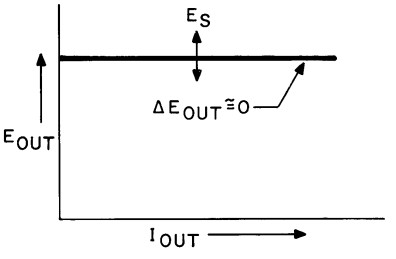
\includegraphics[scale=0.5]{./imagenes/salidaidealfuentedc.jpg}
    \caption{Voltaje de tensión constante salida de fuente ideal.}
    \label{F:salidaidealfuentedc}
\end{figure}

\subsection{Técnicas de Regulación}\par 
La mayoría de las fuentes de alimentación de voltaje constante actuales emplean una de estas cuatro técnicas de regulación:
\begin{itemize}
    \item Serie (Lineal).
    \item Pre-regulador/Regulador en Serie.
    \item Conmutación.
    \item SCR.
\end{itemize}\par 

El objetivo principal de este documento no es proporcionar una explicación exhaustiva de cada uno de estos modelos. En su lugar, se hará una mención breve de todos ellos y se identificará específicamente el modelo que tiene mayor relevancia para los fines de este estudio. Esta aproximación permitirá centrar el análisis en el modelo más pertinente, sin desviar la atención hacia detalles que, aunque importantes, no son esenciales para los propósitos de este trabajo.


\subsection{Fuentes de alimentación lineales.} \par 
Las fuentes de alimentación lineales son un elemento fundamental en la mayoría de los dispositivos electrónicos que utilizamos en nuestra vida cotidiana. Estas fuentes convierten la energía de la red eléctrica en una forma estable y utilizable, proporcionando la energía necesaria para el funcionamiento de los circuitos electrónicos. \par
Una fuente de alimentación lineal consta de varios componentes básicos, como el transformador, el rectificador, el filtro y el regulador de voltaje. Cada uno de estos elementos juega un papel fundamental en garantizar que la energía suministrada sea constante y adecuada para los dispositivos electrónicos, asegurando su correcto funcionamiento.

\section{Funcionamiento básico.} \par 
El tipo más simple y común de fuentes de alimentación de corriente continua (CC) es un sistema \entreComillas{lineal} , mostrado esquemáticamente en la Figura \ref{F:componentesFL}. Primero, se utiliza un transformador para \entreComillas{reducir} la tensión de línea de CA a un voltaje pico más pequeño, que generalmente es aproximadamente 3 voltios superior que el voltaje de salida de CC deseado. Luego, un circuito de diodos rectifica la señal de CA, produciendo una forma de onda con una gran componente de CC. Seguidamente, se utiliza un banco de filtros de condensadores para \entreComillas{suavizar} o \entreComillas{filtrar} la sinusoidal rectificada. \par 
Bajo condiciones de carga normales, siempre hay alguna variación periódica residual o \entreComillas{ripple} en la señal filtrada. Si la aplicación requiere un ripple muy bajo y una salida de CC constante sobre un amplio rango de condiciones de carga, entonces se requiere regulación activa para reducir o eliminar aún más este ripple residual. \cite{tektronix_pws4305}
\begin{figure}
    \centering
    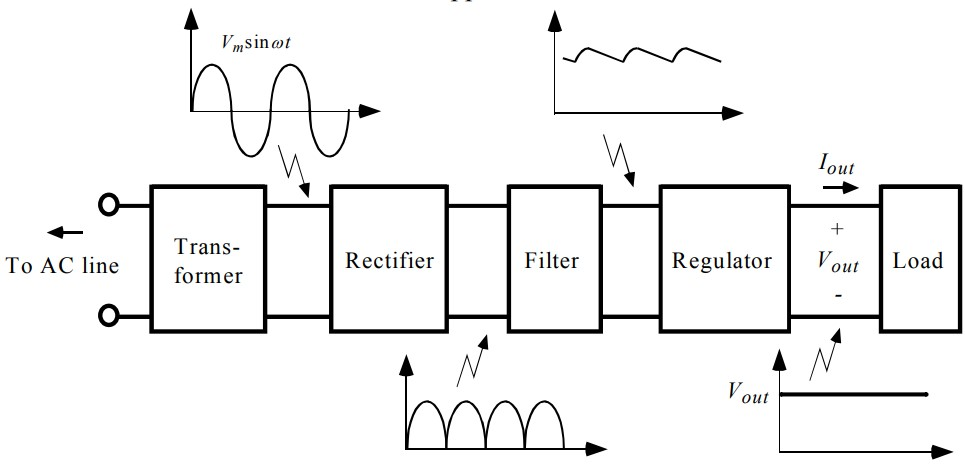
\includegraphics[scale=0.5]{./imagenes/componentesFL.jpg}
    \caption{Diagrama de bloques de una fuente de tensión.}
    \label{F:componentesFL}
\end{figure}

\subsection{Transformador}\par 
El transformador es uno de los componentes principales de una fuente de alimentación lineal. Su función principal es transformar la corriente alterna (CA) de la red eléctrica en una corriente alterna con un voltaje específico adecuado para la aplicación. Consiste en dos bobinas de alambre enrolladas alrededor de un núcleo de hierro, donde la relación entre el número de vueltas en las bobinas determina la relación de transformación del voltaje.

\subsection{Rectificador}\par 
El rectificador es otro componente esencial que convierte la corriente alterna en corriente continua (CC). Esto se logra mediante diodos rectificadores, que permiten que la corriente fluya en una sola dirección. Los rectificadores pueden ser de media onda o de onda completa, dependiendo de cómo se utilizan los diodos para rectificar la señal de entrada.

\subsection{Filtro}\par 
Después de que el rectificador convierte la corriente alterna en corriente continua, la señal resultante puede contener fluctuaciones no deseadas o rizado. Para eliminar estas fluctuaciones y obtener una salida de voltaje suave y constante, se utiliza un filtro. El filtro puede estar compuesto por capacitores y bobinas para eliminar el rizado y suavizar la salida de voltaje.

\subsection{Regulador}\par 
El regulador es el componente final de una fuente de alimentación lineal y se utiliza para mantener constante la salida de voltaje independientemente de las variaciones en la entrada de voltaje o en la carga. Los reguladores de voltaje pueden ser de tipo lineal, que controlan la cantidad de energía disipada como calor para mantener el voltaje de salida constante, o de tipo conmutado, que regulan el voltaje de salida ajustando el ciclo de trabajo de un interruptor.

\section{Ventajas y desventajas}\par 
Todo dispositivo cuenta con una serie de características que la hacen una opción dominante por sobre las demás. Aquí se listan los detalles más dominantes de las fuentes de tensión lineal que las podría hacer preferibles frente a otro tipo de configuraciones.\par 
\underline{Ventajas}:
\begin{itemize}
    \item Simplicidad: Son relativamente simples en diseño y operación.
    \item Bajo ruido: Tienen un nivel de ruido más bajo en comparación con algunas otras formas de fuentes de alimentación.
    \item Baja interferencia electromagnética (EMI): Emiten menos interferencia electromagnética en comparación con las fuentes de alimentación conmutadas.
    \item Buen rendimiento en aplicaciones de baja potencia: Son eficientes y efectivas en aplicaciones de baja potencia.
    \item Buena regulación: Suelen tener una regulación de voltaje estable y precisa.
\end{itemize}\par 
\underline{Desventajas}:
\begin{itemize}
    \item Baja eficiencia energética: Tienen una eficiencia energética más baja en comparación con las fuentes de alimentación conmutadas, especialmente en aplicaciones de alta potencia.
    \item Disipación de calor: Tienden a generar más calor durante la operación debido a la regulación de voltaje a través de dispositivos de regulación lineal, lo que puede requerir disipadores de calor o ventilación adicional.
    \item Mayor tamaño y peso: Suelen ser más grandes y pesadas en comparación con las fuentes de alimentación conmutadas con la misma capacidad de potencia.
    \item Menor rango de voltaje de entrada: Tienen un rango de voltaje de entrada limitado en comparación con las fuentes de alimentación conmutadas, lo que puede limitar su aplicabilidad en ciertos entornos o condiciones de operación.
\end{itemize}

\section{Evolución y mejoras con el pasar de los años}\par 
Las fuentes de corriente directa (CC) han experimentado una evolución significativa desde sus inicios, impulsadas por avances tecnológicos que han mejorado su eficiencia, fiabilidad y capacidad de adaptación a diversas aplicaciones. A lo largo de los años, estas mejoras han permitido que las fuentes de CC se conviertan en componentes esenciales en una amplia gama de dispositivos electrónicos y sistemas de energía. Las mejoras no solamente abarcan mejores materiales sino también el uso de estrategias de control más inteligentes y adaptación para entornos específicos.\par 
Algunas de estas mejoras son:
\begin{itemize}
    \item \textbf{Tecnología de Conversión de Energía}: Las fuentes de CC modernas utilizan técnicas avanzadas de conversión de energía, como la conmutación de alta frecuencia, que permiten una mayor eficiencia energética y una reducción en el tamaño de los dispositivos. La tecnología de conversión resonante, como los convertidores LLC (Inductor-Inductor-Capacitor), ha mejorado la eficiencia en aplicaciones de alta potencia al minimizar las pérdidas por conmutación \cite{zhang2013}.
    \item \textbf{Materiales de Banda Ancha}: La incorporación de materiales semiconductores de banda ancha, como el carburo de silicio (SiC) y el nitruro de galio (GaN). Estos materiales permiten operar a mayores voltajes y frecuencias, mejorando la eficiencia y reduciendo las pérdidas térmicas. Los dispositivos basados en SiC y GaN son especialmente beneficiosos en aplicaciones de alta potencia y alta densidad \cite{palmour2019}.
    \item \textbf{Integración de Funcionalidades Inteligentes}: Las fuentes de CC actuales incorporan funcionalidades inteligentes, como el monitoreo y control digital en tiempo real, que optimizan el rendimiento y la eficiencia energética. Estas fuentes pueden ajustar dinámicamente sus parámetros de operación en respuesta a las condiciones de carga, mejorando así la fiabilidad y prolongando la vida útil de los componentes conectados \cite{brown2020}.
    \item \textbf{Reducción del Tamaño y Peso}: Los avances en diseño y materiales han permitido la reducción significativa del tamaño y peso de las fuentes de DC. Esto es crucial en aplicaciones donde el espacio es limitado, como en la electrónica de consumo portátil y los vehículos eléctricos. La miniaturización también ha facilitado la integración de fuentes de DC en dispositivos médicos y aplicaciones aeroespaciales \cite{kumar2017}.
    \item \textbf{Energía Renovable y Almacenamiento}: Las fuentes de CC han evolucionado para integrarse de manera más efectiva con sistemas de energía renovable y almacenamiento de energía. Las mejoras en la gestión de energía y la capacidad de interactuar con baterías avanzadas y sistemas de almacenamiento han sido vitales para aplicaciones en redes inteligentes y micro-redes \cite{hoffmann2021}.
\end{itemize}\par 
\section{Fuentes comerciales}\par 
Para aquellos lectores interesados en profundizar en el tema abordado en este informe, se sugiere explorar una variedad de fuentes comerciales disponibles en el mercado. A continuación, se presenta una lista de modelos seleccionados que consideramos pertinentes para realizar comparaciones y análisis exhaustivos. Esta selección no solo busca satisfacer el interés académico, sino también proporcionar una base sólida para el estudio y evaluación crítica de las distintas opciones comerciales. Cabe destacar que no existe un producto que sea universalmente perfecto, y, en caso de existir, su costo probablemente no sería accesible para todo tipo de usuario. En este sentido, la elección de una opción sobre otra dependerá en gran medida de las necesidades y preferencias particulares de cada caso. \par 
\begin{table}[h!]
    \centering
    \caption{Características de diversos modelos de fuentes de alimentación.}
    \label{tab:fuentes_alimentacion}
    \begin{tabular}{|p{3cm}|p{3cm}|c|p{5cm}|}
        \hline
        \textbf{Nombre del Modelo} & \textbf{Tensión de Salida} & \textbf{Corriente Máxima} & \textbf{Característica Principal} \\ \hline \hline
        Agilent (Keysight) E3630A & ±25V, 0-6V & 7A (6V), 1A (±25V) & Precisión y fiabilidad, usada en laboratorios e industria \\ \hline
        Tektronix PWS4305 & 0-30V & 5A & Interfaz fácil de usar y salida precisa \\ \hline
        BK Precision 1621A & 0-18V & 3A & Diseño robusto y eficiente en limitación de corriente \\ \hline
        Rigol DP832 & 0-30V (ch1 y ch2), 0-5V (ch3) & 3A (todos los canales) & Interfaz gráfica avanzada, múltiples canales de salida \\ \hline
        GW Instek GPS-3030DD & 0-30V & 3A & Simplicidad y fiabilidad para uso general \\ \hline
        Rohde \& Schwarz HMP2020 & 0-32V (ch1 y ch2) & 10A (ch1 y ch2) & Alta capacidad de corriente y características avanzadas \\ \hline
    \end{tabular}
\end{table}





\chapter{Modificación de la Fuente CC anterior}
% ----------------------

\label{C:Sobre la fuente anterior}

\section{Sobre la fuentes de alimentación anterior}
La revisión y adaptación del trabajo previo titulado \entreComillas{Diseño y construcción de una fuente de alimentación CC lineal con control digital de tensión y corriente} llevado a cabo por Eduardo Javier Matijak y Joaquín Pelinski, documentado en su publicación \cite{Fuente2023}, sirve como punto de partida para comprender las mejoras implementadas en la fuente de alimentación DC que se examina en este informe. \textbf{Invitamos cordialmente al lector interesado a consultar dicho trabajo para obtener una comprensión más completa de los fundamentos sobre los cuales se basa este análisis.} \par 
Esta sección se centra en analizar y discutir las modificaciones realizadas en la fuente de alimentación, específicamente la transición de su mayoría analógica a una configuración digital. Entre los principales cambios introducidos se destacan los siguientes aspectos:

\subsection{Circuito Fijador de Referencia para los Transistores}
El circuito fijador de referencia para los transistores ha sido modificado para incorporar la salida de un Convertidor Analógico-Digital (DAC). El DAC es ahora responsable de aplicar niveles de voltaje acorde a los valores determinados por el control digital. Esta modificación permite un ajuste preciso y programable de las referencias de voltaje, eliminando la necesidad de ajustes mecánicos, por ende mejorando la precisión y flexibilidad del sistema.
\begin{figure}[H]
    \centering
    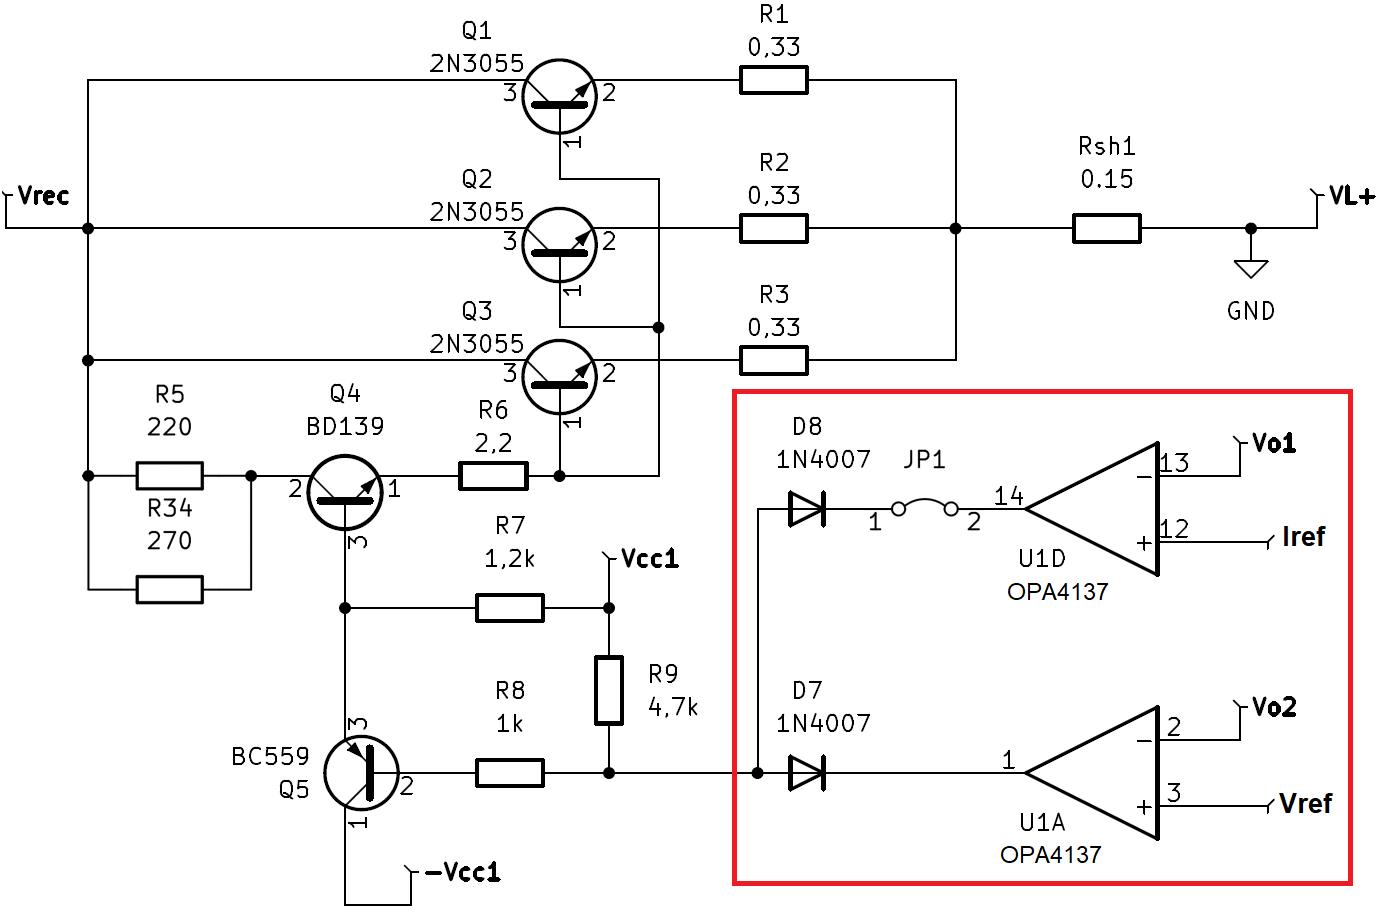
\includegraphics[width=0.8\textwidth]{./imagenes/Eliminada1.PNG}
    \caption{Sección de referencia de tensión a aplicar sobre la base de los transistores.}
    \label{F:Eliminada1}
\end{figure}\par 
Entre los cambios a realizarse a la Figura \ref{F:Eliminada1} se incluye la sustitución de la resistencia de \textit{pull-up} R9 por una de \textit{pull-down}. Se agrega además un seguidor de tensión del voltaje de salida del DAC que inyecte la misma magnitud sobre la base del transistor Q5.

\subsection{Modificación de uso de Potenciómetros Digitales MCP4661}
Originalmente, los potenciómetros digitales MCP4661 se utilizaban para establecer una referencia de voltaje que comandaba los transistores, definiendo tanto la tensión como la corriente sobre la carga. Sin embargo, con la incorporación del DAC, esta función ya no es necesaria. En su lugar, los potenciómetros digitales ahora se utilizan para establecer una referencia de tensión destinada a un circuito de protección analógica contra cortocircuitos. Esta reasignación permite una respuesta inmediata para proteger la carga, evitando los retrasos inherentes a los cálculos y actualizaciones de salida necesarios en un sistema de control digital.
\begin{figure}[H]
    \centering
    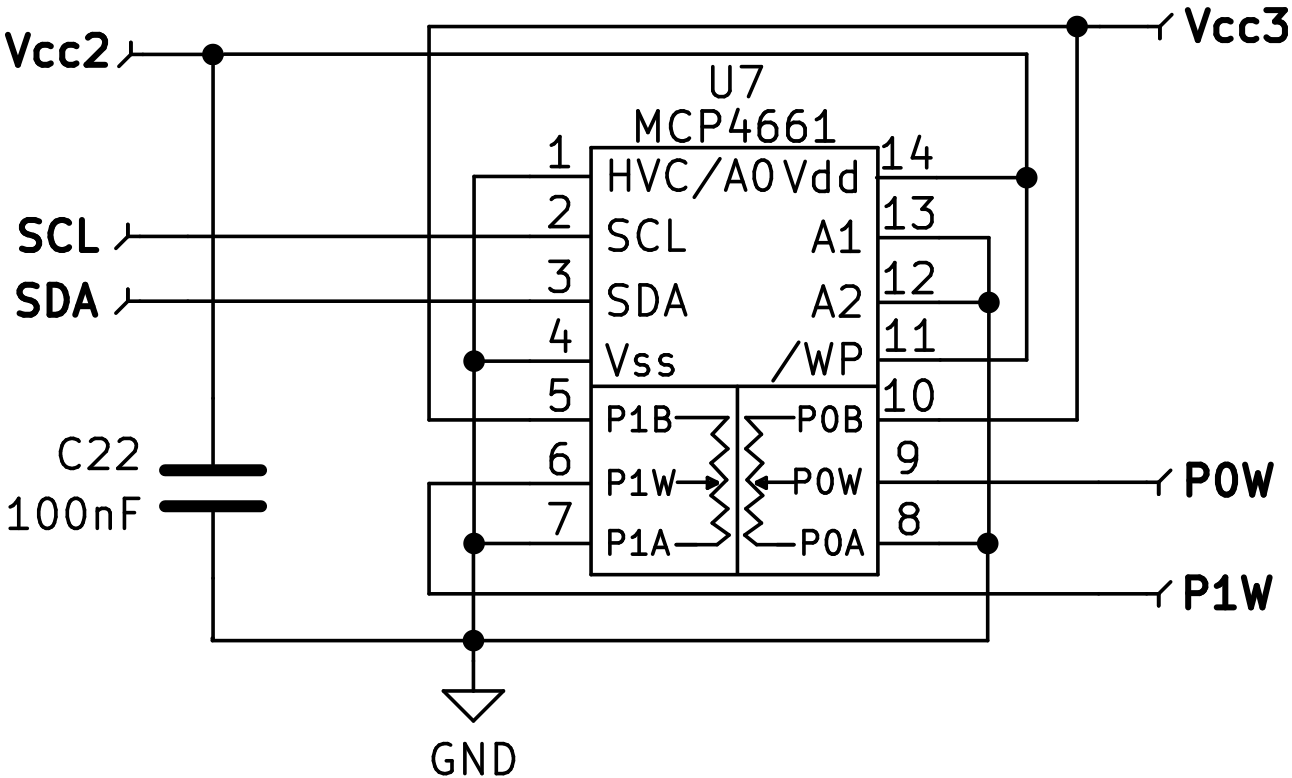
\includegraphics[width=0.5\textwidth]{./imagenes/potenciometro_digital.png}
    \caption{Símbolo del potenciómetro digital MCP4661.}
    \label{F:potenciometro_digital}
\end{figure}
En la Figura \ref{F:potenciometro_digital} podemos observar el símbolo del potenciómetro mencionado. Con el mismo es posible modificar el porcentaje de resistencia mediante comunicación digital a través del protocolo \entreComillas{Circuito Inter-Integrado} (I2C).

\subsection{Eliminación del circuito de medición externo}
Dado que la fuente de alimentación ahora cuenta con una pantalla integrada que muestra en tiempo real los valores de tensión y corriente, el circuito dedicado a la conexión de un voltímetro-amperímetro digital se ha considerado innecesario y, por lo tanto, ha sido eliminado. Esta simplificación reduce la complejidad del diseño y el número de componentes necesarios reduciendo los costos constructivos de la fuente.
\begin{figure}[H]
    \centering
    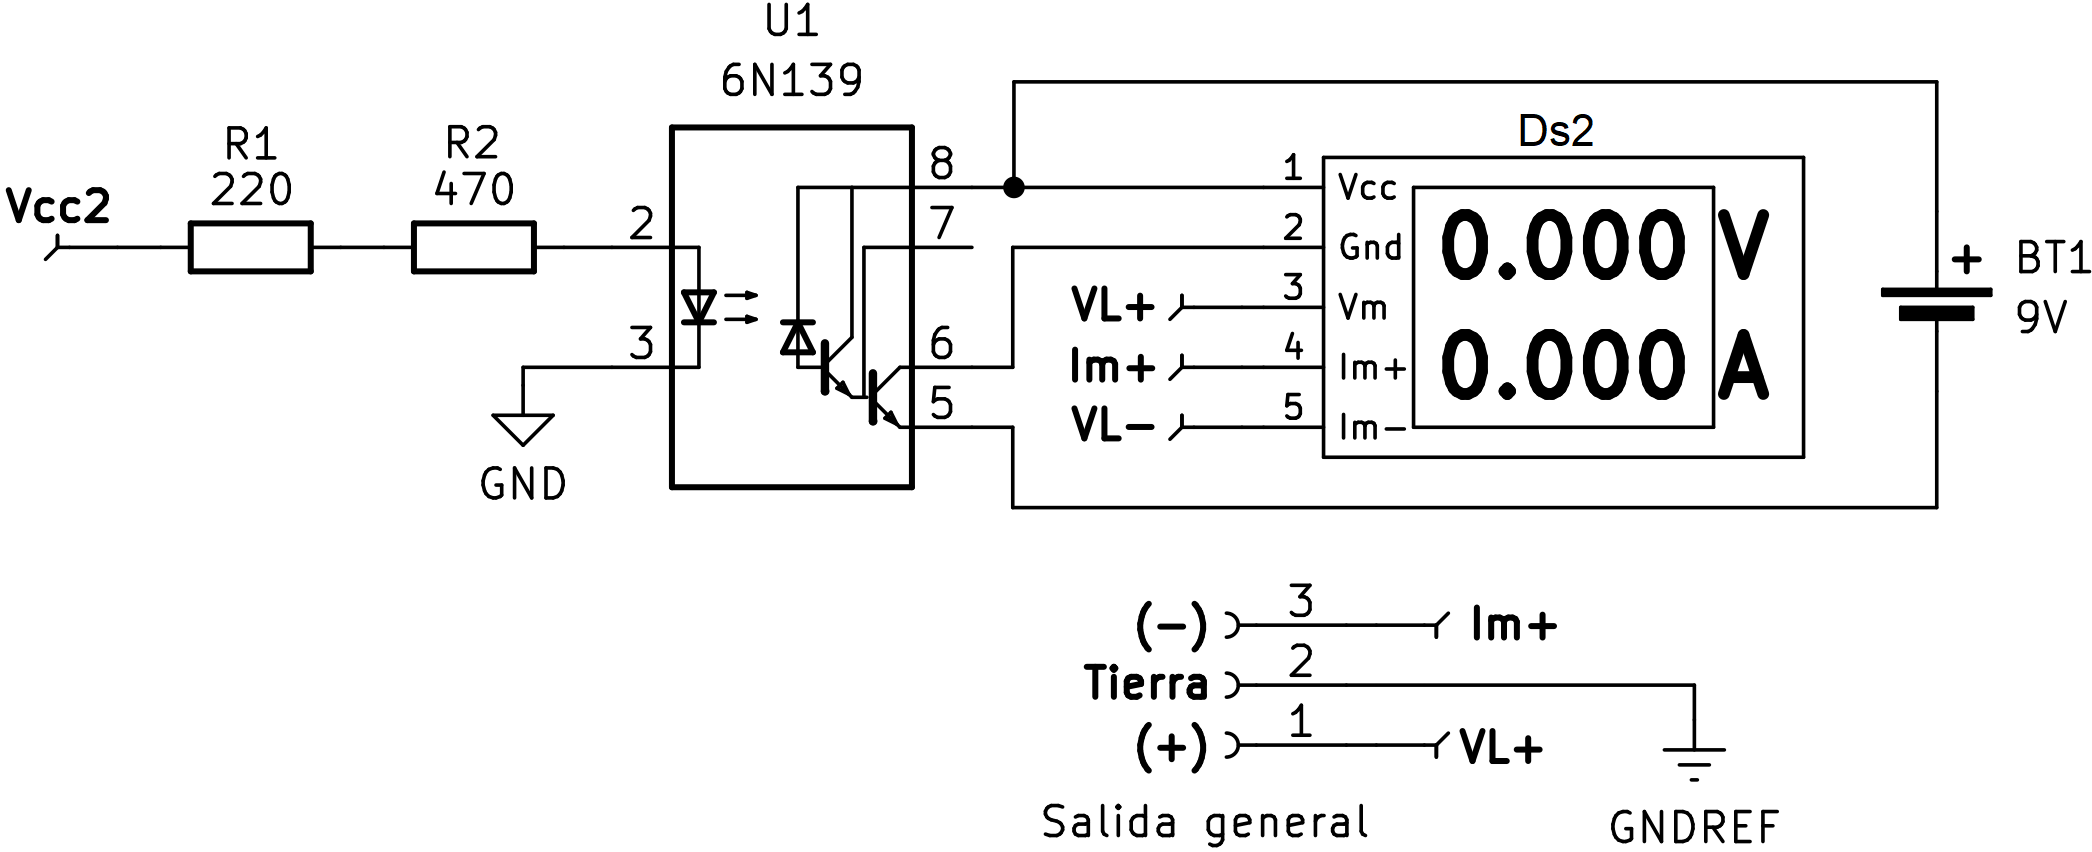
\includegraphics[width=0.8\textwidth]{./imagenes/voltimetro_amperimetro.png}
    \caption{Conexión voltímetro/amperímetro.}
    \label{F:voltimetro_amperimetro}
\end{figure}
En la Figura \ref{F:voltimetro_amperimetro} se aprecia los interconexión de los elementos que conformaban esta etapa. También se resalta que para su correcto funcionamiento era necesario una batería de 9V.

\subsection{Modificación del Circuito de Acople y Desacople de Carga}\par 
Se ha modificado considerablemente el circuito de disparo del relé de acople y desacople de carga, aprovechando las capacidades proporcionadas por el "Arduino Nano" con sus entradas y salidas digitales.
\begin{figure}[H]
    \centering
    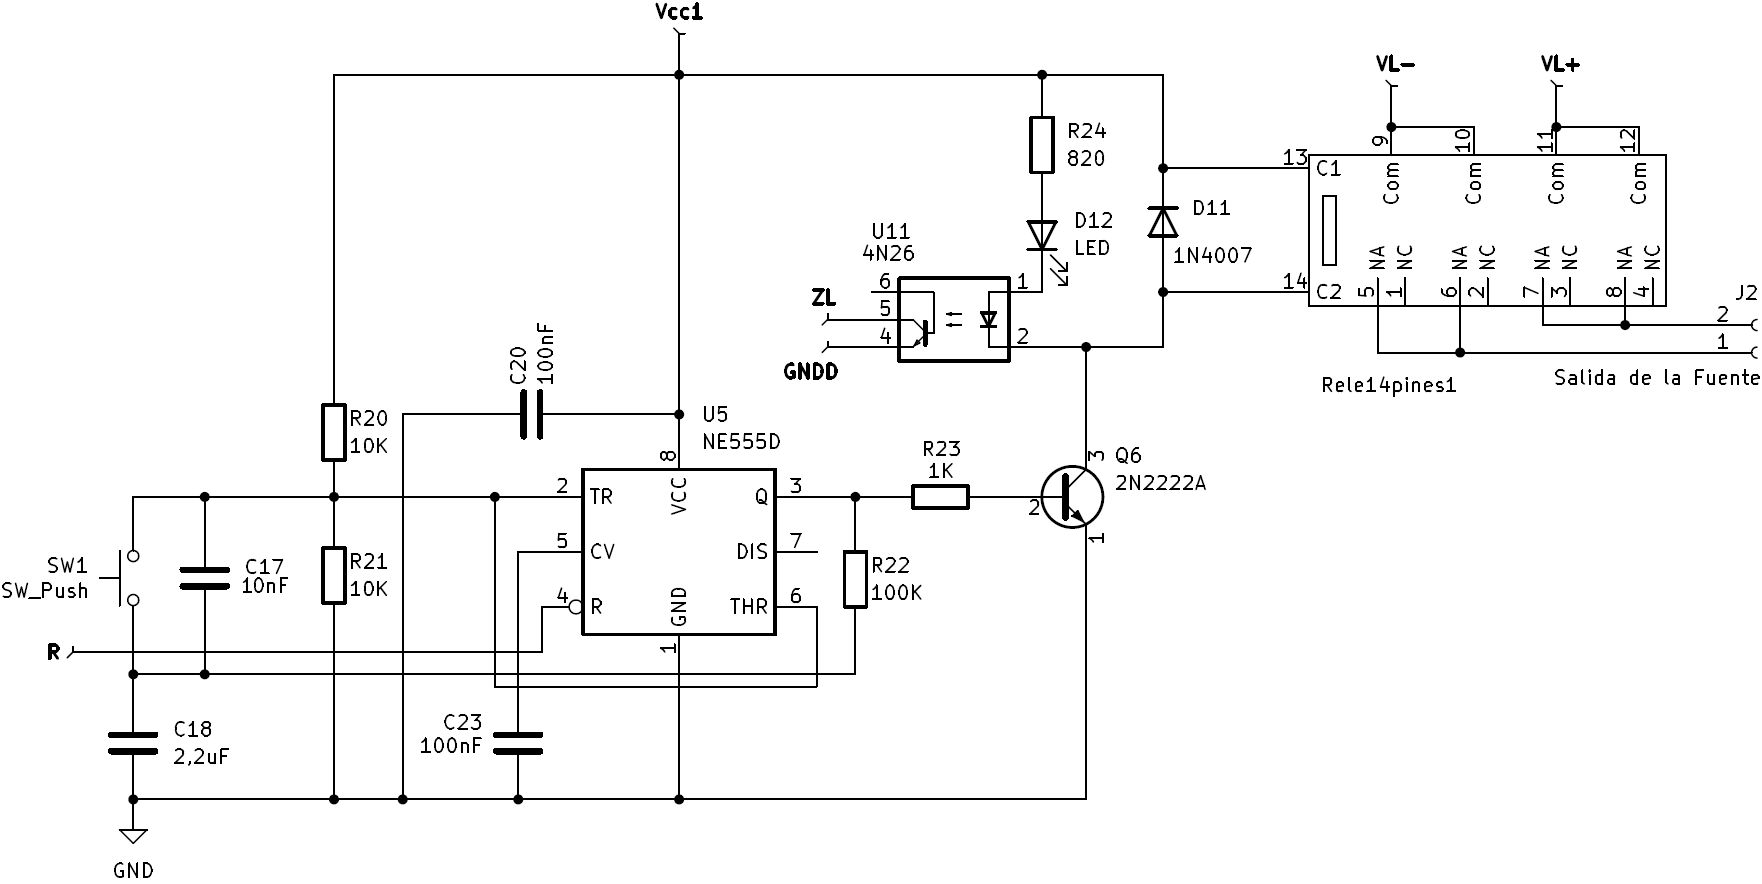
\includegraphics[width=0.9\textwidth]{./imagenes/conexion_carga.PNG}
    \caption{Acople y desacople de carga.}
    \label{F:conexion_carga}
\end{figure}\par 
En la Figura \ref{F:conexion_carga} se presenta el esquema utilizado por la fuente anterior. Gracias a las características del microcontrolador es posible prescindir del NE555 en cuanto a la temporización se refiere. Sin embargo, se sigue requiriendo el uso de optoacopladores para mantener la aislación entre la etapa de potencia y la etapa digital.

\subsection{Simplificación del Circuito Indicador de Modo de Operación}
La pantalla integrada también cumple la función de indicar el modo de operación, eliminando la necesidad de un circuito adicional dedicado a esta tarea. Esto no solo simplifica el diseño del sistema, sino que también mejora la experiencia del usuario al centralizar toda la información relevante en un solo lugar.
\begin{figure}[H]
    \centering
    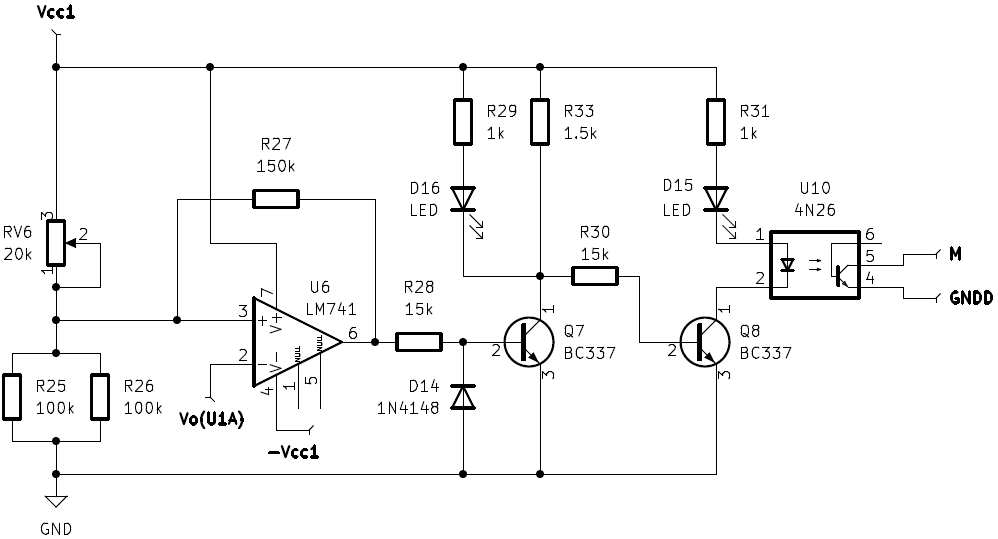
\includegraphics[width=0.9\textwidth]{./imagenes/modo_operacion.PNG}
    \caption{Sección de referencia de tensión.}
    \label{F:modo_operacion}
\end{figure}

\subsection{Integración del Circuito con NodeMCU ESP-32S}
Dado que no se requiere una conexión inalámbrica según las especificaciones del circuito, se ha prescindido del microcontrolador ESP con módulo Wi-Fi que tenía como objetivo la visualización de la información en un display, leer el estado de los \textit{encoders} rotativos y registrar los datos mas relevantes. Para mantener la aislación utilizaba el circuito integrado ISO1540 \cite{ISO1540}. El esquemático del circuito registrador que utilizaban puede observarse en la Figura \ref{F:ESP_32S}.
\begin{figure}[H]
    \centering
    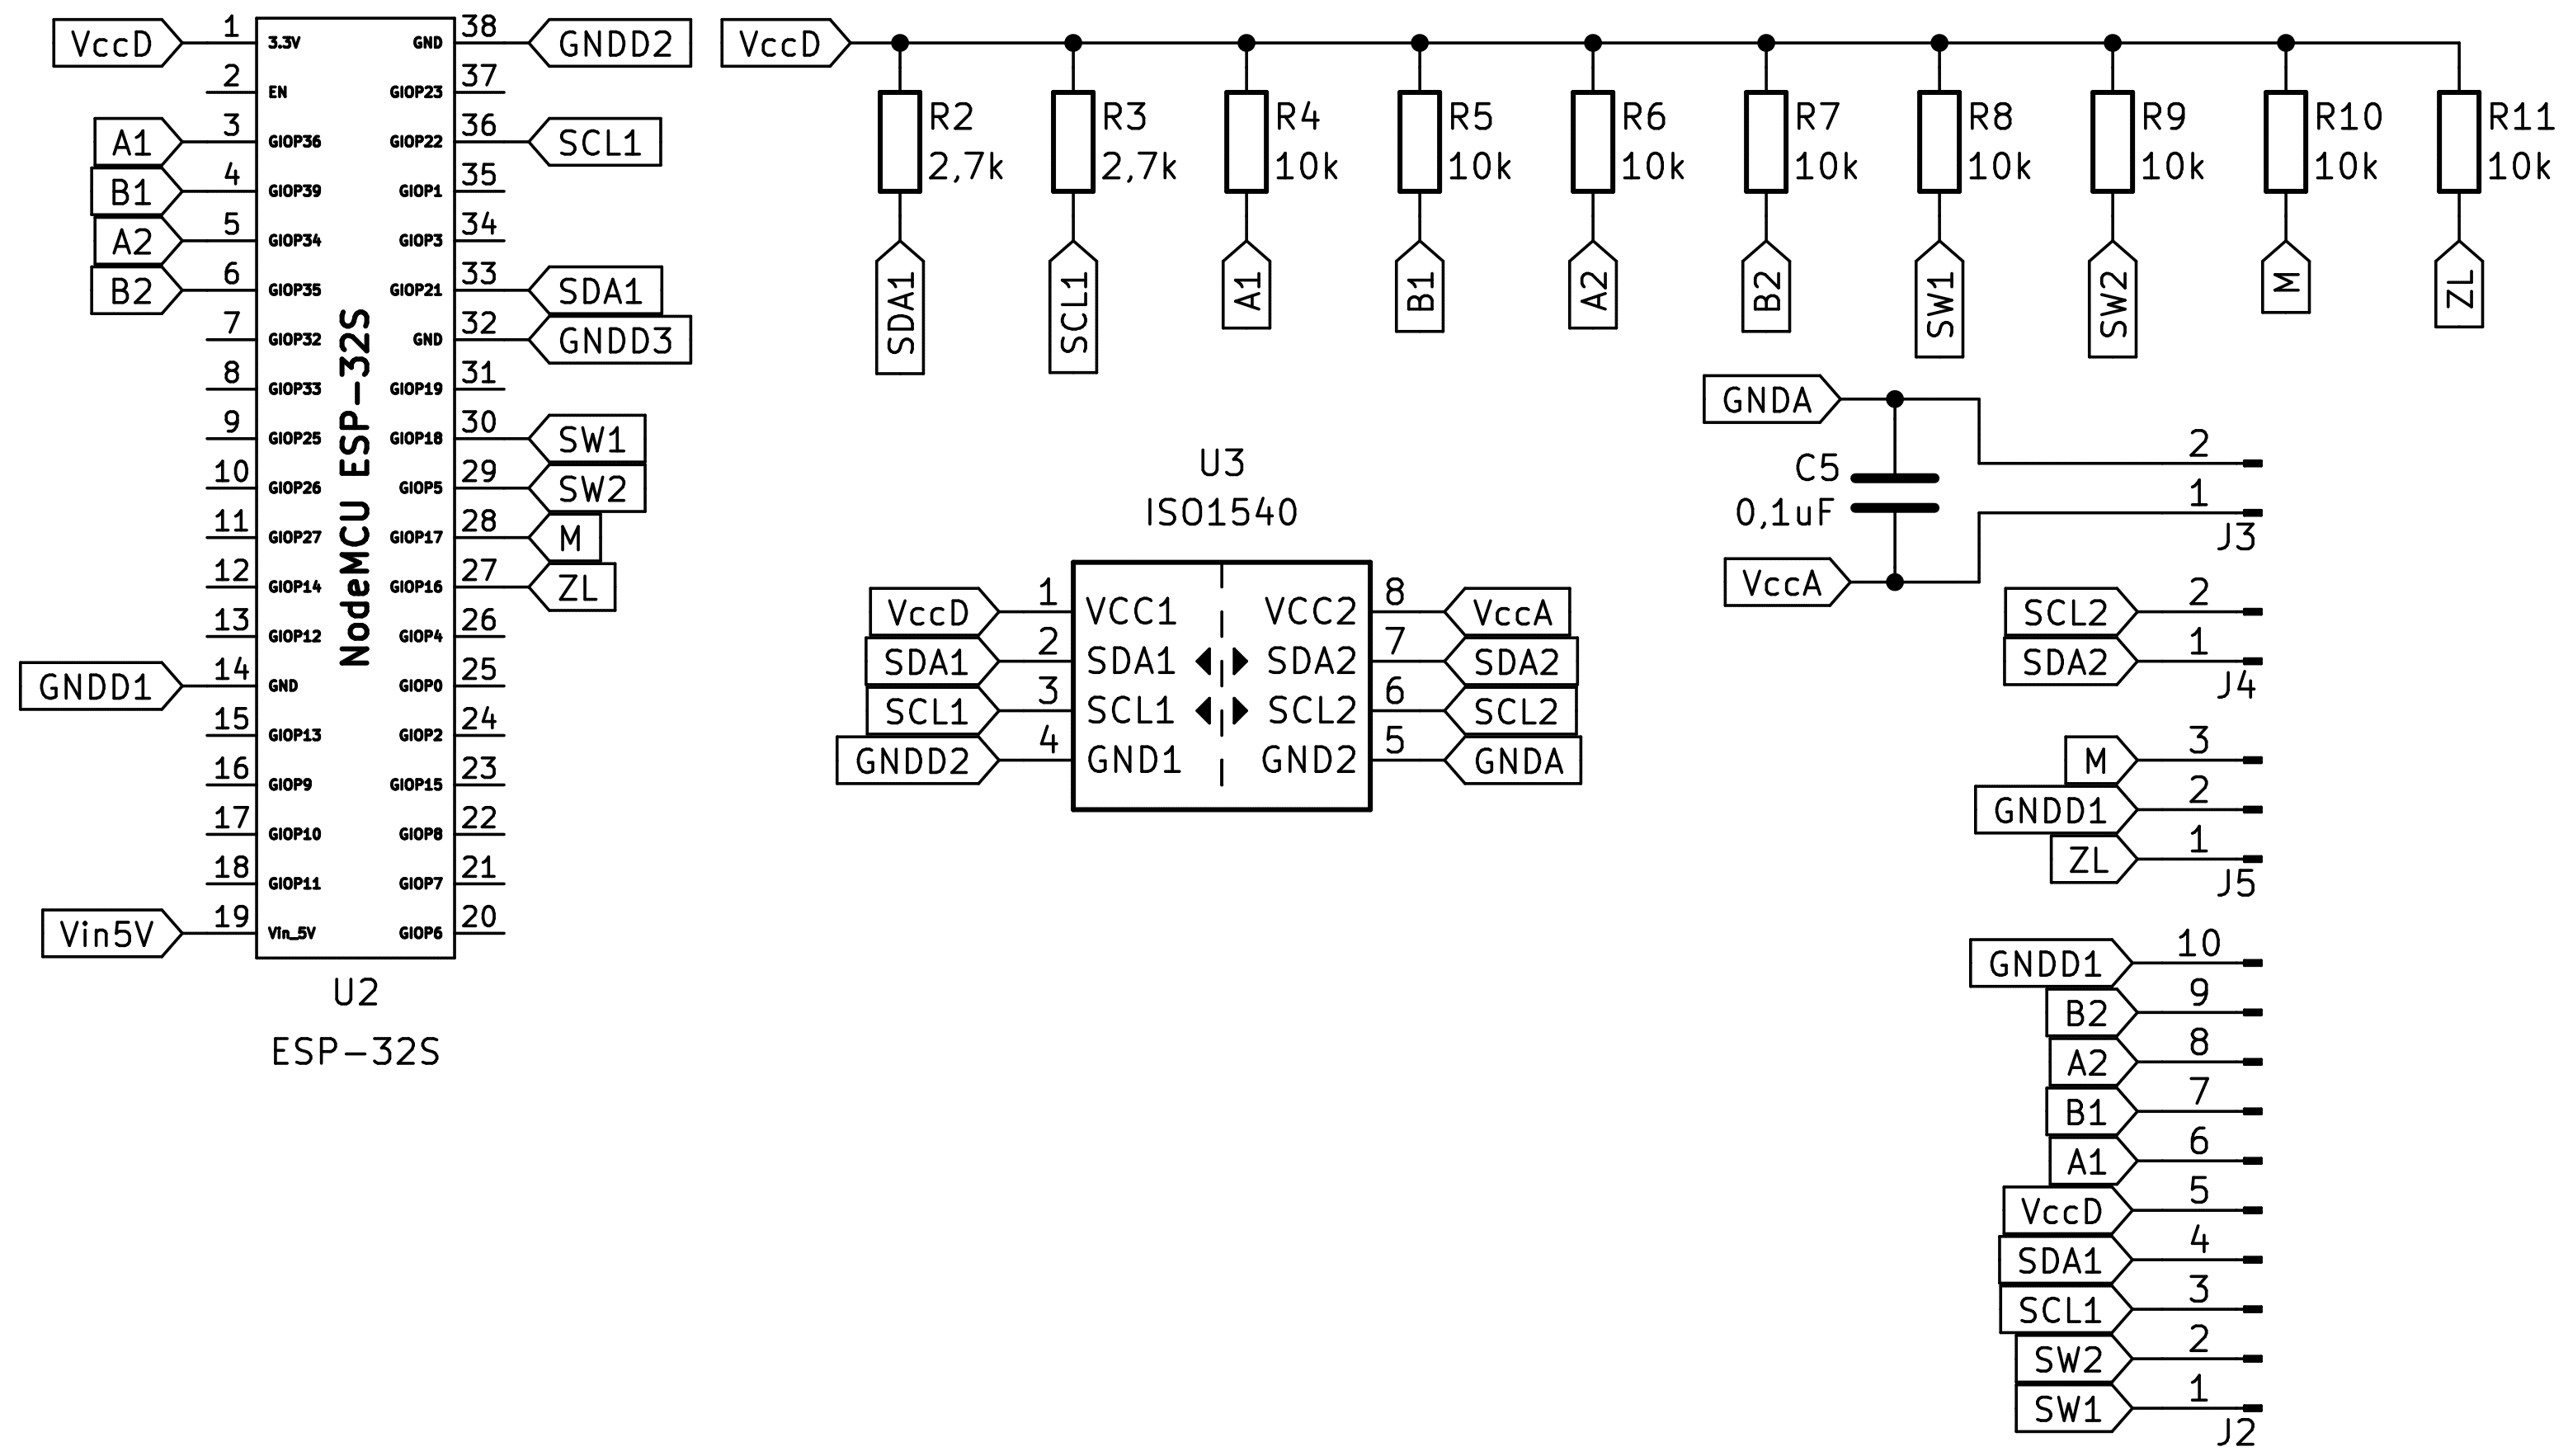
\includegraphics[width=0.8\textwidth]{./imagenes/ESP_32S.png}
    \caption{Circuito registrador de datos.}
    \label{F:ESP_32S}
\end{figure}

\subsection{Encoders rotativos}\par 
El uso de un teclado numérico hace que este elemento se vuelva totalmente innecesario para estas aplicaciones dado a que el objetivo de la fuente es que sea totalmente digital evitando el ajuste manual de las magnitudes. Sin embargo, no habría problema en dejar este elemento en paralelo en caso de requerir una alternativa para la fijación de las magnitudes. Esto se debe a una cuestión tradicional ya que la gran mayoría de los usuarios están acostumbrado a \textit{setear} manualmente las fuentes de tensión mediante perillas.
\begin{figure}[H]
    \centering
    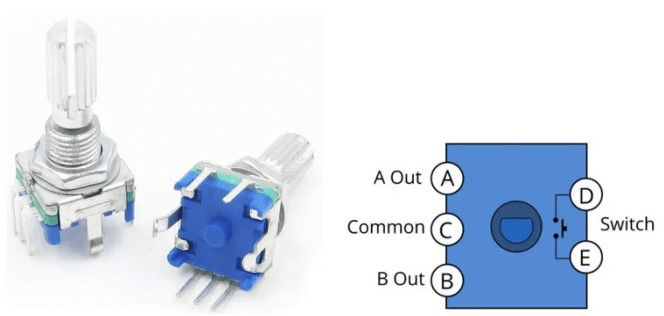
\includegraphics[scale=0.5]{./imagenes/encoder_rotativo.jpg}
    \caption{Encoder rotativo.}
    \label{F:encoder_rotativo}
\end{figure}
\ 
\ 
\par 
Estas modificaciones han permitido no solo modernizar la fuente de alimentación, sino también mejorar su funcionalidad y eficiencia mediante la incorporación de tecnología digital y la simplificación de circuitos redundantes. En las secciones siguientes, se detallarán en profundidad cada uno de estos cambios y su impacto en el rendimiento general del equipo






% ----------------------
  \chapter{Diseño del prototipo}



% ----------------------
\section{Etapa de alimentación} \par
Para la alimentación de los amplificadores operacionales que se utilizarán para el sensado de la tensión y corriente, además de los demás componentes que lo requieran, se realiza el diseño de una fuente de continua partida de $\pm 12V$ y una fuente simple de $+5V$ obtenida a partir de los $+12V$ regulados. \par
\begin{figure} [H]
	\centering
	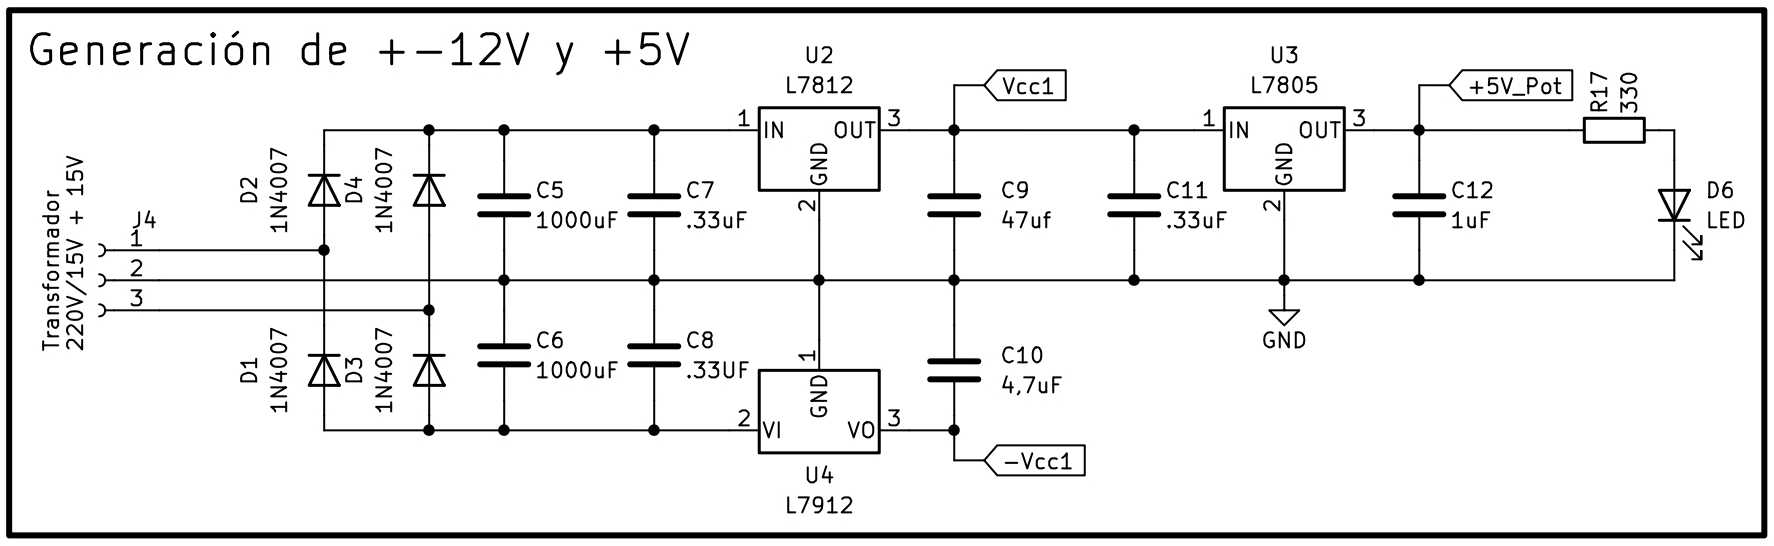
\includegraphics[width=\textwidth]{./imagenes/Alimentacion_analogica.png}
	\caption{Fuente de alimentación de los componentes}
	\label{F:alimentacion_analogica}
\end{figure} \par 
Se cuenta con un transformador de $220V/(15+15)V$. Por lo que definiendo los capacitores $C_5 =C_6 =1000\mu F/25V$ y una corriente máxima supuesta de $500mA$ se tiene una tensión eficaz de \textit{ripple} de:
\begin{equation}
	V_{ripple} =\frac{0,5A}{4\cdot \sqrt{2}\cdot (50Hz)\cdot (1000\mu F)}=1,7677V
\end{equation} \par
Considerando la caída de tensión de un diodo como $V_D =0,7V$ obtenemos la expresión del valor medio de la tensión rectificada:
\begin{equation}
V_{alim} =V_{trafo} \cdot \sqrt{2}-2\cdot V_D -V_{ripple} \cdot \sqrt{2}=(15\cdot \sqrt{2})-(2\cdot 0,7V)-(1,77V\cdot \sqrt{2})=17,31V
\end{equation} \par
En paralelo a los capacitores $C_5$ y $C_6$ se agregan los capacitores $C_7$ y $C_8$ de $0,33\mu F/25V$ para eliminar los ruidos de alta frecuencia según la aplicación recomendada en la hoja de datos del LM78XX [INSERTAR REFERENCIA]. Para los diodos rectificadores se emplean 1N4007.\par
Para fijar el valor de voltaje de salida se emplean los integrados LM7812 y LM7912 de +12V y -12V respectivamente. A continuación se colocan capacitores de desacople con el fin de mejorar la estabilidad y reducir el ruido. Asegurando un suministro de tensión estable y confiable para los demás componentes electrónicos conectados al sistema. \par 
A la salida de la fuente de alimentación de +12V se conecta el regulador, LM7805, para obtener +5V regulados con su correspondiente capacitor de salida de $C_{sal} =1\mu F$. Por ultimo se conecta un LED, en conjunto con una resistencia limitadora, para indicar el correcto funcionamiento de la etapa de alimentación. \par 
\begin{equation}
R_{lim} =\frac{(+5V)-V_{LED} }{I_{LED} }=\frac{(+5V)-(2V)}{10mA}=300\Omega \to 330\Omega
\end{equation} \par 
\begin{equation}
P_{R_{lim} } =\frac{(+5V-2V)^2 }{330\Omega }\cdot 1,5=40,9mW\to 1/8W
\end{equation}

\section{Etapa de Potencia}\par

Para la etapa de potencia se hace uso de un transformador de 220V / 33V siendo el circuito de rectificación y filtrado el que se aprecia a continuación:

\begin{figure} [H]
	\centering
	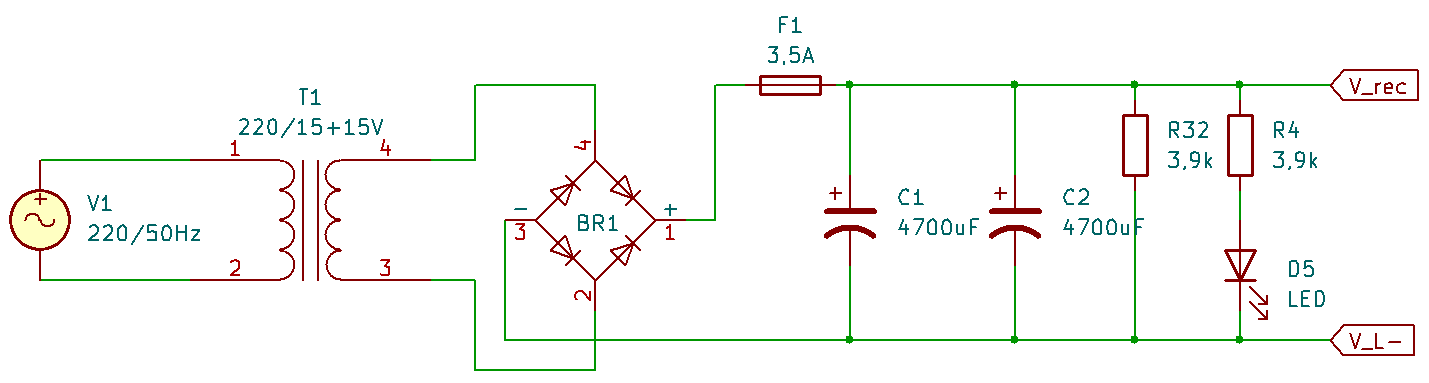
\includegraphics[width=\textwidth]{./imagenes/Rectificador_potencia.png}
	\caption{Circuito de rectificación y filtrado de la etapa de potencia}
	\label{F:rectificador_potencia}
\end{figure} \par 

Se diseña esta etapa para obtener un bajo valor de tensión de \textit{ripple} y que pueda entregar una corriente de 3 A. Para dimensionar el valor del capacitor a utilizar se hace uso de la siguiente expresión:
\begin{equation}
C=\frac{3A}{4\sqrt{2}(50Hz)(\frac{3V/2}{\sqrt{2}})}=1000\mu F
\end{equation} \par 

A partir de este cálculo adoptamos 2 capacitores en paralelo: $C_1 =C_2 =4700~\mu F~/~63~V$, con lo cual la tensión pico a pico de \textit{ripple} resulta de  $V_{r(pp)} =3,1915~V$. \par 

Esto nos da como resultado un valor medio de tensión rectificada y filtrada para una carga de 3 A de: 
\begin{equation}
V_{rec} =(33\cdot \sqrt{2}V)-2\cdot 0,7V-\frac{3,1915V}{2}=43,67V
\end{equation} \par 

Luego, en paralelo a los capacitores se coloca una resistencia $R=3,9k\Omega /1W$ con el fin de descargar los capacitores en un tiempo $\tau =R\cdot C=(3900\Omega )\cdot (2\cdot 4700\mu F)=36,66s$ cuando se desconecte la fuente de alimentación. La corriente a través de la resistencia cuando la carga no sea de $I_0 =3A$ será de:
\begin{equation}
I_{R32} =\frac{V_{rec} }{R32}=\frac{43,67V}{3900\Omega }=11,2mA
\end{equation}\par 

Mientras que la potencia del resistor se calculará empleando un factor de seguridad de $fs=1,5$: 
\begin{equation}
P_R \ge \frac{V_R^2 }{R}\cdot fs=\frac{(43,67V)^2 }{3900\Omega }\cdot 1,5=0,7336W\to 1W
\end{equation} \par 

Adicionalmente se coloca un LED indicativo de encendido con un resistor limitador de valor: 
\begin{equation}
R_{LED} =\frac{V_{rec} -V_{LED} }{I_{LED} }=\frac{43,67V-2V}{10mA}=4167,33\Omega \to 3900\Omega
\end{equation} \par 

\section{Sensado de corriente}
En esta etapa se emplea una resistencia de \textit{Shunt} $R_{sh1} =0,15~\Omega$ para obtener un voltaje proporcional a la corriente que está circulando por la misma. Luego para elevar el valor del mismo en torno a los 5 V cuando estén circulando 3 A por la misma se utiliza un amplificador operacional en una configuración de amplificador no inversor, dada por la siguiente expresión:
\begin{equation}
V_{o1} =V_{NI} \times (1+\frac{R_{V4} }{R_{14} })=(I_L \times R_{sh1} )\times (1+\frac{R_{V4} }{R_{14} })
\end{equation}\par 

\begin{figure} [H]
	\centering
	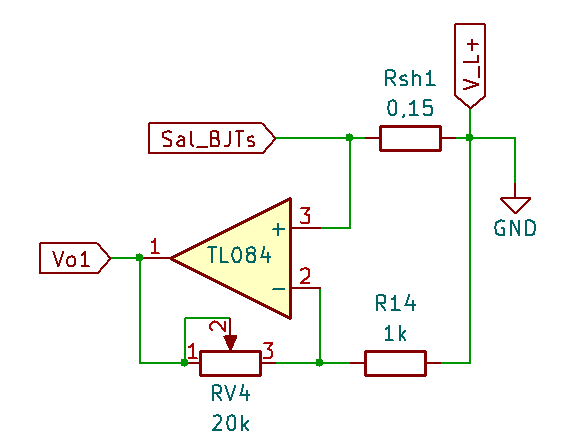
\includegraphics[width=0.6\textwidth]{./imagenes/Sensor_corriente.png}
	\caption{Circuito de sensado de la corriente de salida}
	\label{F:Sensor_corriente}
\end{figure} \par 

Cuando circule $I_L =3A$ por $R_{sh1}$ obtendríamos un voltaje en la entrada no inversora de $V_{NI} =3A\cdot 0,15\Omega =0,45V$ por lo que adoptando el resistor $R_{14} =1k\Omega$ y calibrando el potenciómetro $R_{V4} $ a $10k\Omega$ obtenemos como resultado para fondo de escala una tensión de:
\begin{equation}
V_{o1} =(0,45V)\cdot (1+\frac{10k\Omega }{1k\Omega })=4,95V
\end{equation} \par 

Se coloca el preset RV4 con el fin de poder calibrar el voltaje de salida $V_{o1}=5V$ para una corriente $I_L=3A$. Las potencias de las resistencias se obtienen como:
\begin{equation}
P_{Rsh1}\geq I_L^2\cdot Rsh1\cdot 1,5=(3 A)^2\cdot (0,15 \Omega)\cdot 1,5\cong 2 W \to P_{Rsh1}=2W
\end{equation}
\begin{equation}
P_{R14}\geq \frac{V_I^2}{R_{14}}\cdot 1,5=\frac{(0,45 V)^2}{1000\Omega}\cdot 1,5 \cong 0,3 mW \to P_{R14}=1/8W
\end{equation} \par

\section{Sensado de tensión}
Se requiere un circuito que convierta los niveles de tensión de la salida. Para ello se presenta el circuito a continuación, en el cual se puede variar la ganancia del sistema ajustando el potenciómetro RV1.
\begin{figure} [H]
	\centering
	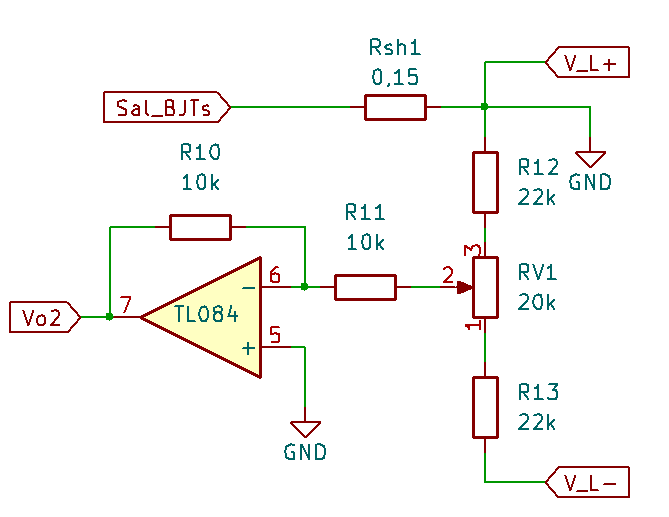
\includegraphics[width=0.6\textwidth]{./imagenes/Sensor_tension.png}
	\caption{Circuito de sensado de la tensión de salida}
	\label{F:Sensor_tension}
\end{figure} \par 

Debido a que el punto común de referencia ($0 V$) de las fuentes de $\pm 12V$ coincide con el borne positivo $V_{L+}$ de salida de la fuente lineal, el borne opuesto respecto a GND será de hasta $V_{L-}=-30V$. Como el valor leído desde el cursor de RV1 es negativo, para poder ser comparado con la referencia es necesario invertir su signo mediante un amplificador inversor con ganancia unitaria. \par 

Estableciendo el valor de las resistencias $R_{12}=R_{13}=22k\Omega$ y despreciando la corriente que fluye a través del cursor del preset RV1 hacia la entrada de alta impedancia del amplificador operacional, la corriente a través de $R_{12}$, $R_{13}$ y $RV1$ para $V_L=30V$ será de:
\begin{equation}
I_{R12}=\frac{V_L}{R12+RV1+R13}=\frac{30 V}{(2\cdot 22000+20000)\Omega}\cong 469\mu A
\end{equation} \par 

Por lo tanto, las potencias resultan de
\begin{equation}
P_{R12}\geq (I_{R12})^2\cdot R12\cdot fs=(469\mu F)^2\cdot (22000 \Omega)\cdot 1,5 \cong 7,6 mW \to P_{R12}=P_{R13}=P_{RV3}=1/8W
\end{equation} \par 

Mientras que se definen las resistencias $R10=R11=10 k\Omega \ 1/8W$ debido a que la corriente que circulan por ellas es despreciable.\par 

\section{Actuador de potencia} \par 

El circuito observado en la Figura \ref{F:Circuito_Actuador} tiene la finalidad de controlar la tensión y corriente de salida. Se denota que se conecta el punto de referencia (GND) a la salida de tensión positiva con el fin de poder utilizar los amplificadores operacionales en torno a este punto de mayor potencial, requiriendo fuentes sencillas de $\pm12V$.

\begin{figure} [H]
	\centering
	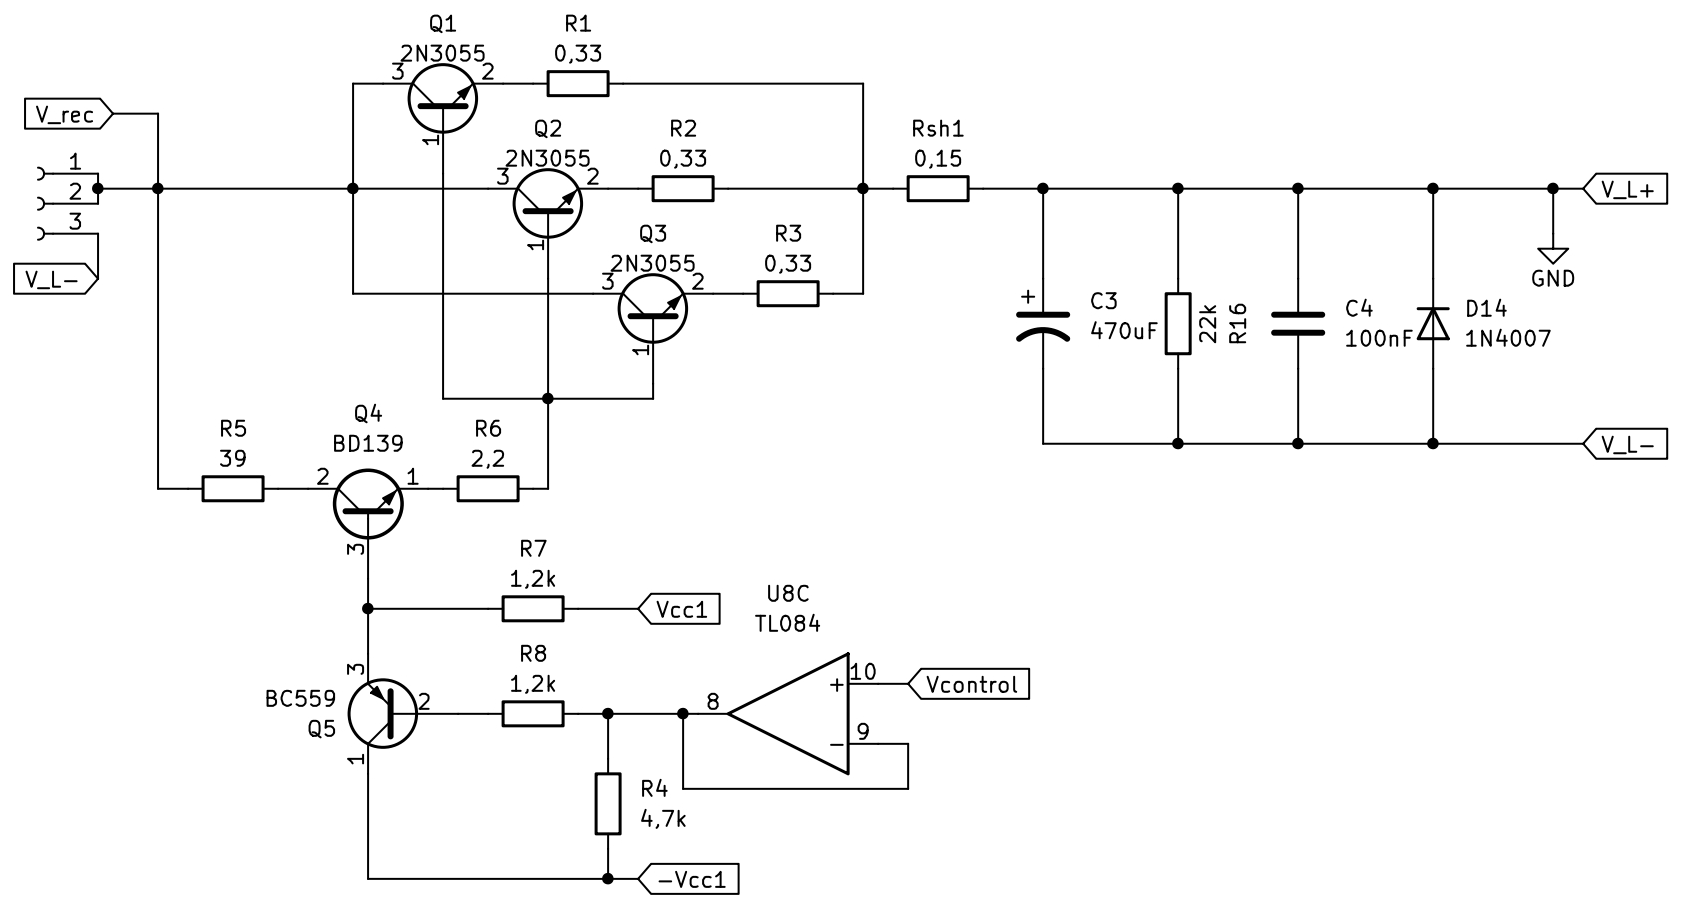
\includegraphics[width=\textwidth]{./imagenes/Circuito_actuador.png}
	\caption{Regulador de tensión con transistores de paso.}
	\label{F:Circuito_Actuador}
\end{figure} \par 

Se utilizó como transistor de potencia tres 2N3055 conectados en paralelo, con ganancia $h_{FE1} =20$ y $V_{BE1(ON)} =1,5~V$ mientras que para accionarlo se utiliza un BD139 con $h_{FE4} =30$ y $V_{BE4(ON)} =1V$. \par 
Considerando el caso de máxima carga $V_L =30V$ y $I_L =3A$ en la base de los transistores debe haber una tensión igual a:
\begin{equation}
\begin{split}
V_{B1}&=V_L+I_L\cdot Rsh1+\frac{I_L}{3}\cdot R1+V_{BE1(on)}= \\
&=(30V)+(3A)\cdot (0,15\Omega)+(1A)\cdot (0,33\Omega)+(1,5V)=32,28V
\end{split}
\end{equation} \par 

Se procede a calcular la corriente de colector a pasar por el transistor BD139 para alcanzar la excitación de los transistores de potencia dada la expresión:
\begin{equation}
I_{C4}=\frac{I_L}{hfe1}=\frac{3A}{20}=0,15A
\end{equation} \par 

Se adopta una resistencia $R6=2,2\Omega$ como resistencia de emisor para estabilización térmica y $V_{CE4}=5V$ para un funcionamiento en zona activa. Por lo que podemos calcular R5 como:
\begin{equation}
R_5=\frac{V_{rec}-V_{CE4}-V_{B1}}{I_C4}-R_6=\frac{43,67 V-5V-32,28V}{0,15A}-2,2\Omega=40,42\Omega \to 39\Omega 
\end{equation} \par 

Verificando las potencias:
\begin{equation}
P_{R5}\geq (0,15A)^2\cdot (39\Omega)\cdot 1,5=1,364 W \to P_{R5}=2W
\end{equation}
\begin{equation}
P_{R6}\geq (0,15A)^2\cdot (2,2\Omega)\cdot 1,5=74,25 mW \to P_{R5}=1/8W
\end{equation} \par

Para el cálculo del disipador del BD139 (Q4) se supone el caso en que ocurre un corto-circuito a la salida de la fuente, actuando el control de corriente manteniendo estable la corriente en $I_L=3A$ y la tensión $V_L=0V$. Por lo que la tensión de colector-emisor de Q4 será:
\begin{equation}
\begin{split}
V_{CE4max}&=V_{rec}-I_{C4}\cdot (R5+R6)-V_{B1}=\\
&=43,67V-0,15A\cdot (39+2,2)\Omega -2,28V=35,21 V
\end{split}
\end{equation} \par 

Se calcula la potencia que debe disipar el transistor Q4:
\begin{equation}
\begin{split}
P_{Q4}&=V_{CE4(max)}\cdot I_{C(max)}+V_{BE(on)}\cdot \frac{I_{C(max)}}{hfe4}=\\
&=35,21V\cdot 0,15A+1V\cdot \frac{0,15A}{40}=5,28W
\end{split}
\end{equation} \par 

Como la potencia que debe disipar es mayor a la que puede soportar sin disipador ($1 W$ extraído de la hoja de datos), resulta necesario dimensionar un disipador. Para ello se emplea la temperatura de juntura máxima ($T_{J4}=150^\circ C$), la resistencia térmica juntura-carcasa para el encapsulado TO-126 ($\theta _{JC}=10^\circ C/W$), la resistencia térmica carcasa-disipador (en este caso, pasta térmica $\theta _{CD}=1^\circ C/W$) y se supone una temperatura ambiente $T_A=50^\circ C$. Por lo que la resistencia térmica disipador-ambiente debe ser igual o menor que:
\begin{equation}
\begin{split}
\theta_{DA} &= \frac{T_J-T_A}{P_{Q4}}-\theta_{JC}-\theta_{CD}=\\
&= \frac{(150-50)^\circ C}{5.28W}-(10^\circ C/W)-(1^\circ C/W)=7.92^\circ C/W
\end{split}
\end{equation} \par
 
A continuación se procede a calcular las resistencias R7, R8 y R9. Para R7 se supone el caso de $V_L=30 V$ y $I_L=3 A$ donde la corriente de colector del transistor Q4 es de $I_{C4}=150 mA$. Dada una ganancia de $hfe4=40$ la corriente de base de este transistor será:
\begin{equation}
I_{B4}=\frac{I_{C4}}{hfe4}=\frac{150mA}{40}=3,75mA
\end{equation}\par

Suponiendo que la corriente de emisor de Q5 es igual a la corriente de base de Q4, es decir $I_{E5}=I_{B4}=3,75mA$, tenemos que la corriente a través de R7 será $I_{R7}=I_{B4}+I_{E5}=7,5mA$. Paso siguiente, se determina la tensión en la base de Q4:
\begin{equation}
V_{B4}=V_{B1}+I_{C4}\cdot R_6+V_{BE4}=32,28V+(0,15A\cdot 2,2\Omega)+1V=33,61V
\end{equation}\par

Debido a que el punto de referencia ($GND=0V$) de la fuente de $\pm 12V$ coincide con el borne positivo de $V_{L+}$ de la fuente de salida de $V_L=30V$, entonces el nivel de tensión de $V_cc1$ respecto al borne negativo $V_{L-}$ es de $V'_{cc1}=V_{cc1}+V_L=12V+30V=42V$. Por lo que la resistencia R7 puede calcularse como:
\begin{equation}
R7=\frac{V_{cc1}-V_{B4}}{I_{R7}}=\frac{42V-33,61V}{7,5 mA}=1118 \Omega \to 1200\Omega
\end{equation}\par 

Para el cálculo de R8 establecemos que $I_L=0A$ de modo que la base de Q4 tenga un potencial próximo a los $0V$, donde podemos adoptar un potencial de aproximadamente $0,8V$. Esto provoca que el BD139 esté en corte, y la tensión y corriente de salida sean nulas. Por lo que en este caso, toda la corriente que circula a través de R7 corresponde a la corriente de emisor de Q5. Por lo que:
\begin{equation}
I_{R7(max)}=\frac{V_{cc1}-V_{B4(min)}}{R7}=\frac{12V-0,8V}{1200}\cong 9,33 mA
\end{equation} \par 
El transistor Q5 es un BC559 y tiene una ganancia $hfe5=110$ y una tensión emisor-base $V_{EB5}=0,7V$ con la cual la resistencia R8 resulta:
\begin{equation}
R8=\frac{V_{B4}-V_{EB5}}{(\frac{I_{R7}}{hfe5})}=\frac{0,8V-0,7V}{(\frac{9,33 mA}{110})}=1178,57\Omega \to 1200\Omega
\end{equation}\par 

La resistencia R9 es una resistencia de \textit{pull-down} que tiene la utilidad de dejar establecido un valor de tensión a la base de Q5 en caso que se desconecte el controlador. Por lo tanto, podemos calcular su valor suponiendo que por la misma no va a circular más que unos $I_{R9}=2,5 mA$ cuando el voltaje en el punto superior se encuentre a $0V$.
\begin{equation}
R9=\frac{V_C-(-V_{cc1})}{I_R9}=\frac{0V-(-12V)}{2,5 mA}=4800\Omega \to 4700\Omega 
\end{equation}\par 

A continuación se calcula las potencias a disipar por las resistencias R7, R8, R9 y el transistor Q5. Se consideran los escenarios donde circula la mayor corriente, donde para R9 se puede suponer un caso extremo de $V_{B(extremo)}=-12V$. Mientras que para el transistor se supone $V_{CE5(max)}=5V$:
\begin{equation}
P_{R7}\geq (9,33mA)^2\cdot (1200\Omega )\cdot 1,5=156,8 mW	\to P_{R7}=1/4W
\end{equation}
\begin{equation}
P_{R8}\geq (\frac{9,33mA}{110})^2\cdot (1200\Omega )\cdot 1,5= 13\mu W \to P_{R8}=1/8W
\end{equation}
\begin{equation}
P_{R9}\geq \frac{(12V-0V)^2}{1200\Omega}\cdot 1,5=183,82 mW	\to 	P_{R9}=1/4W
\end{equation}
\begin{equation}
P_{Q5}=(5V\cdot 9,33mA)+0,7V\cdot \frac{9,33mA}{110}\cong 46,73mW
\end{equation}\par 

De la hoja de datos de Q5 tenemos que $P_{Q5(max)}=500mW$, por lo que se cumple que $P_{Q5}<P_{Q5(max)}$. Respecto a la potencia disipada en R1, R2 y R3 que se corresponden con las resistencias de emisor de los transistores de potencia, su corriente máxima será de $I_{L(max)}/3=1A$, por lo que:
\begin{equation}
P_{R1}\geq (1A)^2\cdot (0,33\Omega)\cdot 1,5=495 mW \to P_{R1}=P_{R2}=P_{R3}=1W
\end{equation}\par 
La máxima disipación de potencia en los transistores Q1, Q2 y Q3 está dado para el caso de $I_L=3A$ cuando $V_L=0V$, que ocurre ante un cortocircuito a la salida. En este caso, tenemos una tensión (despreciando caída en diodos rectificadores) de $V_{CE1} = (43,67 V)-(0,33 V)-(0,45 V)=42,89 V$ y una corriente de colector de $I_{C1(max)}=1 A-(1A/20)=950mA$. Por lo que la potencia que disipa será:
\begin{equation}
P_{Q1}=(42,89V\cdot 0,95A)+1,5V\cdot \frac{0,95A}{20}=40,82 W
\end{equation}\par 
Se calcula si el transistor podrá disipar esa potencia sin disipador conociendo que su resistencia térmica de juntura-ambiente es de $\theta _{JA}=20^\circ C/W$ y la temperatura máxima de juntura es $T_J=200^\circ C$ y la temperatura ambiente se establece en $T_A=50^\circ C$.
\begin{equation}
P_{Q1(SD)}=\frac{(200-50)^\circ C}{20^\circ C/W}=7,5W \to P_{Q1}>P_{Q1(SD)} \to \text{Requiere disipador}
\end{equation} \par 
Se dimensiona el disipador conociendo que la resistencia térmica juntura-carcasa es $\theta_{JC}=1,5^\circ C/W$ y la resistencia térmica carcasa-disipador es $\theta_{CD}=0,5^\circ C/W$ (contacto con grasa y arandela de mica).
\begin{equation}
\theta_{DA1}=\frac{(200-50)^\circ C}{40,82 W}-(10^\circ C/W)-(0,5^\circ C/W)=1,655^\circ C/W
\end{equation}
Por lo que se requiere un disipador con una resistencia térmica igual o menor que $\theta_{DA1}=1,655^\circ C/W$.

\section{Acople y desacople de carga}
Para conectar y desconectar la carga se utiliza un relé de salida. El mismo será accionado cuando el usuario lo determine luego de establecer los valores deseados de tensión y/o corriente de salida. El circuito puede apreciarse en la Figura \ref{F:Circuito_Acople_carga}.

\begin{figure} [H]
	\centering
	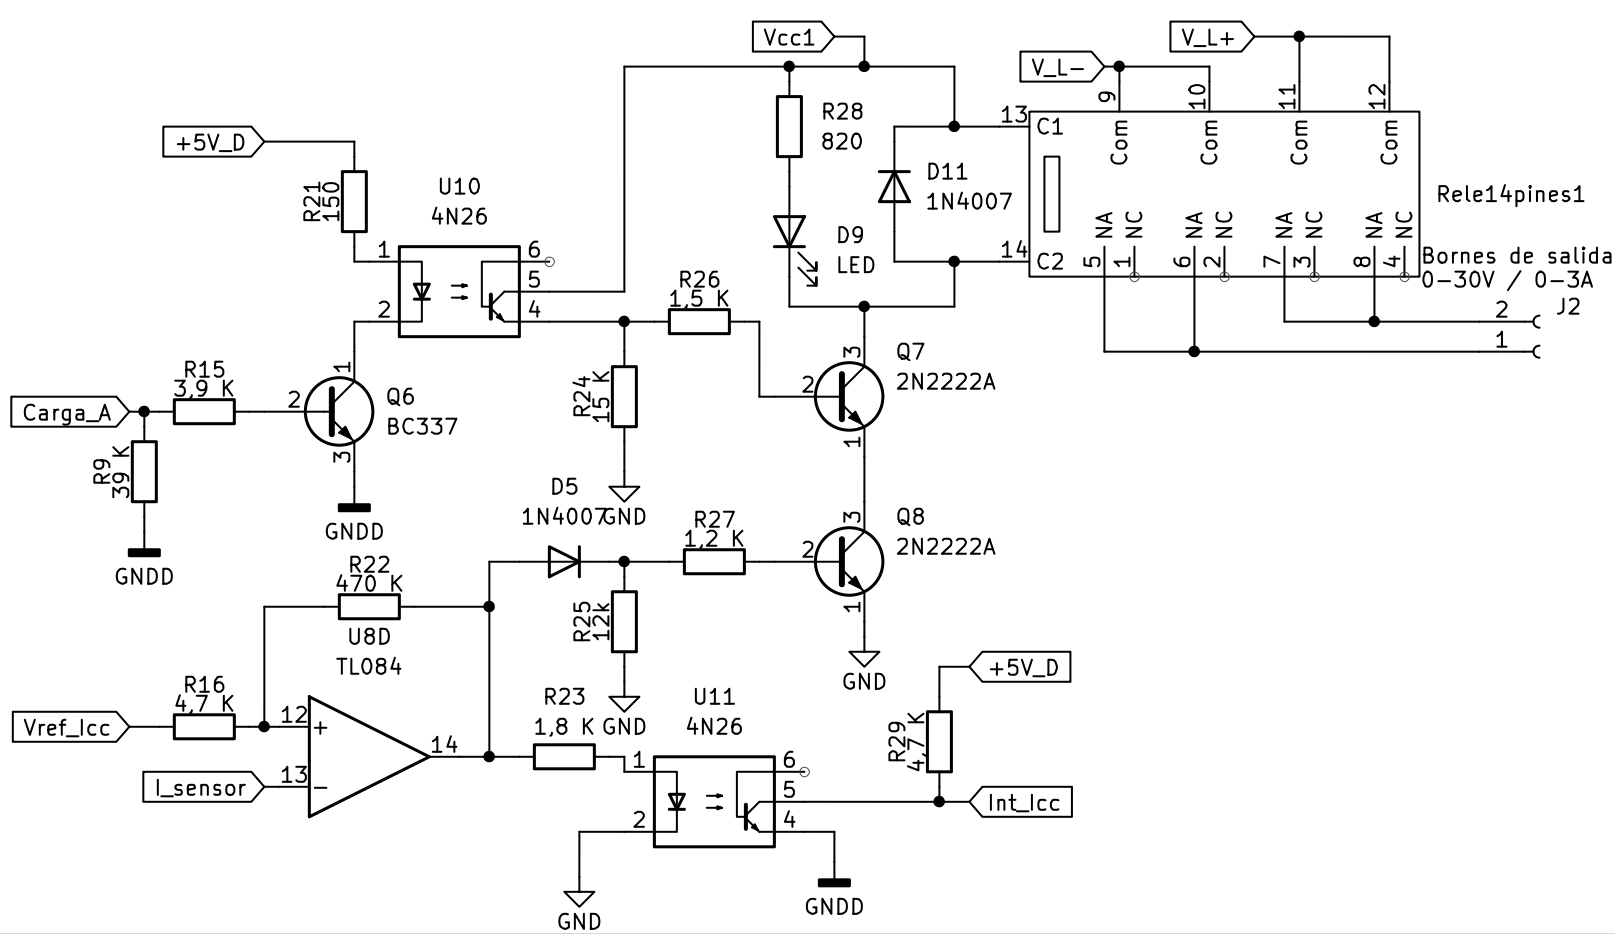
\includegraphics[width=\textwidth]{./imagenes/Acople_carga.png}
	\caption{Circuito de acople y desacople de carga.}
	\label{F:Circuito_Acople_carga}
\end{figure} \par 

Como transistor se utiliza el 2N2222A \cite{2N2222}, el cual soporta las siguientes magnitudes: $V_{CEmax}=40V$; $I_{Cmax}=600 mA$ y $P_{Dmax}=625 mW$. Las características de funcionamiento que presenta son $V_{CE(sat)}=0,3V$; $V_{BE(on)}=1,2V$ y $hfe=100$

\begin{equation}
R_{LED}=\frac{V_{cc1}-V_{LED}-2\cdot V_{CE(sat)}}{I_LED}=\frac{12V-2V-2\cdot 0,3V}{10 mA}=940\Omega \to 820 \Omega
\end{equation}
\begin{equation}
I_{LED}=\frac{V_{cc1}-V_{LED}-2\cdot V_{CE(sat)}}{R_LED}=\frac{12V-2V-2\cdot 0,3V}{820 \Omega}=11,46 mA
\end{equation}
Considerando que la corriente que circula por la bobina del Relé es de $30 mA$, se calculan las resistencias de base de la siguiente manera:
\begin{equation}
I_C=I_{Rele}+I_{LED}=30mA+11,46 mA=41,46 mA
\end{equation}
\begin{equation}
I_B=5\cdot \frac{I_C}{hfe}=5\cdot \frac{41,46 mA}{100}=2,073 mA
\end{equation}
\begin{equation}
	R_{BQ7}=\frac{V_{cc1}-V_{CE(Opto)}-V_{CE(Q8)}-V_{BE(Q7)}}{I_B}=\frac{12V-0,5V-0,3V-1,2V}{2,073mA}=4823 \Omega
\end{equation}
\begin{equation}
	R_{BQ8}=\frac{V_{OH}-V_D-V_{BE(Q7)}}{I_B}=\frac{10V-0,7V-1,2V}{2,073 mA}=3907 \Omega
\end{equation}

Se adopta $R_{BQ7}=1,5 k\Omega$ y $R_{BQ8}=1,2 k\Omega$ para asegurar la saturación. Además se agregan las resistencias R24 y R25 con el fin de que la base de los transistores se mantenga con un nivel de tensión bajo cuando se desea que los mismos permanezcan en corte.\par 
El amplificador operacional TL084 \cite{TL084} que se observa en la Figura \ref{F:Circuito_Acople_carga} se encuentra en la configuración de comparador con histéresis. El mismo se encarga de comparar el voltaje correspondiente a la corriente de salida con un valor de referencia $V_{ref(icc)}$ establecido por el usuario. Este cumple la función de que ante un caso extremo de corriente, desacoplar la carga por seguridad. Además, acciona una interrupción en el microcontrolador indicando el error.\par 



















\chapter{Estrategia de control}
% ----------------------

\label{C:Formas de control}

\section{Principio de estrategia de control.}
El algoritmo PID (proporcional, integral, derivado) está formado por la suma de tres componentes, Proporcional, Integral y Derivativo) Matemáticamente, un controlador PID tiene la siguiente formulación: \par
\begin{equation}
Output(t)=K_p\cdot e(t)+K_i\int_0^t e(t)\cdot dt+K_d\cdot \frac{de}{dt}
\end{equation} \par 
Cada componente del PID es \entreComillas{independiente} de las demás. en el sentido de que cada uno calcula una salida de lo que \entreComillas{para él} debería hacer para obtener la respuesta adecuada. \par 
Los tres componentes se suman para dar la salida del controlador. Cada uno cumple una cierta función y mejoran cierta parte de la respuesta. Y cuando los tres componentes trabajan juntos, en la proporción adecuada, consiguen un gran comportamiento. \par 
Cada componente tiene un parámetro $K_p$, $K_i$ y $K_d$, respectivamente. Estos parámetros indican la ponderación que tiene en el resultado final.
\begin{itemize}
\item El componente proporcional reacciona al presente.
\item El componente integral reacciona al pasado, y aporta “memoria” al controlador.
\item El componente derivado reacciona al futuro, y aporta “predicción” al controlador.
\end{itemize} \par 
Resumiendo los efectos del PID:
\begin{itemize}
\item Componente proporcional:
\begin{itemize}
\item Valor bajo de $K_p$, respuesta lenta.
\item Valor alto de $K_p$, sobrepaso, oscilación, e incluso inestabilidad.
\item No consigue eliminar el error en régimen estacionario.
\end{itemize}
\item Integral:
\begin{itemize}
\item Elimina el error estacionario.
\item Demasiado $K_i$, oscilación e inestabilidad.
\end{itemize}
\item Derivativo:
\begin{itemize}
\item Mejora el comportamiento general
\item Demasiado $K_d$, comportamiento indeseado en la salida.
\item Muy sensible al ruido.
\item Muy sensible a cambios bruscos en el error (perturbaciones o cambios de consigna)
\end{itemize}
\end{itemize}\par 

En base a estos conceptos, se propone el siguiente esquema de control presentado en la Figura \ref{F:Esquema_Control}. En el mismo, los parámetros configurables por el usuario serán la tensión de referencia, la corriente máxima de control y un valor de corriente de cortocircuito que desconectaría la carga por seguridad. \par 

\begin{figure} [H]
	\centering
	\includegraphics[width=\textwidth]{./imagenes/Esquema_Control.jpg}
	\caption{Diagrama de bloques del funcionamiento del controlador.}
	\label{F:Esquema_Control}
\end{figure} \par 
Tanto para el lazo interno de corriente como para el lazo externo de tensión se utilizará un controlador PID. El controlador del lazo de tensión le brindará la corriente de referencia a seguir al lazo de corriente, cuya salida del controlador será el voltaje a aplicar sobre la base del transistor del regulador lineal con BJTs. \par 

La ecuación de un controlador PID en tiempo continuo está dada por: \cite{BotteronSC1}
\begin{equation}
u(t)=K_pe(t)+K_i\int _0^t e(t)dt +K_d\frac{de(t)}{dt}
\end{equation} \par 
Siendo su expresión en el dominio de Laplace:
\begin{equation}
U(s)=(K_p+\frac{K_i}{s}+sK_d)E(s)
\end{equation}\par 
Donde considerando una aproximación rectangular backward, la acción de control resultante en función de la variable 'z' resulta:
\begin{equation}
s\approx\frac{(z-1)}{zT} \quad \to \quad U(z)=[K_p+K_iT\frac{z}{z-1}+\frac{K_d}{T}\frac{(z-1)}{z}]E(z)
\end{equation}\par 
Aplicando la anti-transformada $Z$ a $U(z)$ se obtiene la ecuación a diferencias finitas ya conocida:
\begin{equation}
u(k)=K_pe(k)+K_iT\sum_{n=1}^k e(n)+\frac{K_d}{T}[e(k)-e(k-1)]
\end{equation}\par 
Esta expresión de la acción de control depende del error actual $e(k)$, donde no considera el atraso de implementación digital $T_d$. \par 
Por ello se introduce una predicción del error:
\begin{equation}
e(k)=e(k-1)+[e(k-1)-e(k-2)]
\end{equation}\par 
De esta forma la acción de control depende de los errores anteriores y $u(k)$ no se ve afectada por el atraso de implementación digital, pudiendo compensar eficientemente las perturbaciones. \par 
Por lo tanto, la ecuación a diferencias de la acción de control resulta:
\begin{equation} \label{eq:PIDp}
u_{PIDp}(k)=u_{PIDp}(k-1)+K_1e(k-1)+K_2e(k-2)+K_3e(k-3)
\end{equation}\par 


\section{Lazo de corriente}
Para realizar el diseño del lazo de control interno es necesario realizar un modelado del mismo. Al utilizar diversos softwares de simulación (PSIM y TINA TI), se verificó que efectivamente, mientras se encuentre en la zona lineal los transistores, la corriente de salida dependerá linealmente de la tensión de entrada, $I_L=k\cdot V_{ctrl}$\par 
Sin embargo, determinar el valor de k no es sencillo, dado que en los extremos de la recta de carga, el sistema se vuelve no lineal. Además. existe un cierto valor mínimo en el cual el transistor se mantendrá en corte. Por ende, se asumirá una planta con ganancia unitaria mientras que se retocarán las ganancias del controlador experimentalmente hasta alcanzar la respuesta deseada.\par 

\section{Lazo de tensión}
Para realizar el diseño del lazo de control externo de tensión se modela la carga de salida, obteniendo la función de transferencia que vincule la tensión de salida con su corriente. \par 
Suponiendo una carga Resistiva-Capacitiva (RC) de $C=470\mu F$ y $R=10\Omega$. Por Laplace se establecen las siguientes relaciones:\par 
\underline{Resistencia}:
\begin{equation}
v(t)=i(t)R \Leftrightarrow V(s)=I(s)R
\end{equation}\par 
\underline{Capacitor}:
\begin{equation}
v(t)=\frac{1}{C}\int i(t)dt \Leftrightarrow V(s)=\frac{1}{sC}I(s)+\frac{1}{s}v(0)
\end{equation}

\begin{figure} [H]
	\centering
	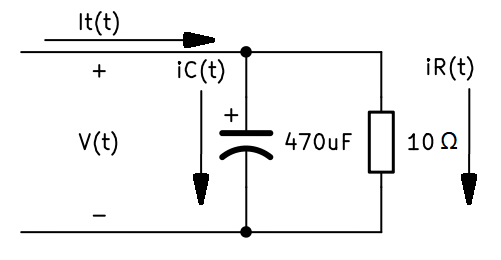
\includegraphics[scale=0.6]{./imagenes/CircuitoRC.png}
	\caption{Modelo de la salida de tensión.}
	\label{F:CircuitoRC}
\end{figure} \par 
Aplicando la ley de Kirchoff para los nodos:
\begin{equation}
i_t(t)=i_R(t)+i_C(t)
\end{equation}\par 
Pasando al dominio de Laplace:
\begin{equation}
I_t(s)=I_R(s)+I_C(s)
\end{equation}\par 
Reemplazando por lo obtenido anteriormente:
\begin{equation}
I_t(s)=\frac{V(s)}{R}+sCV(s)
\end{equation}\par 
Finalmente obtenemos el modelo que define la carga:
\begin{equation}
G_P(s)=\frac{V(s)}{I_t(s)}=\frac{1}{\frac{1}{R}+sC}
\end{equation}\par 
Con este y el lazo cerrado de corriente obtenido en la sección anterior es posible diseñar el control externo de tensión de forma tal que cumpla con ciertas especificaciones de diseño. Es posible utilizar la técnica de reubicación de polos por lugar geométrico de las raíces para obtener las constantes a implementar. \par 
La ecuación a diferencias a utilizar resulta en la presentada en \ref{eq:PIDp}.

\section{Algoritmo Anti-Windup}
La acción de control resultante del PI $u_{PI}(kT_s)$ puede ser saturada o limitada a valores positivos y/o negativos en casos en los que se presentan sobretensiones o sobrecorrientes por encima de los valores permitidos. La limitación de la acción de control a un valor fijo, significa que el sistema pierde la controlabilidad de los estados del proceso dado que sería similar a imponer un valor de referencia fijo; en este caso, esta referencia sería la del lazo interno de control de corriente. Esta situación provoca que el error entre la referencia y la salida varíe, tanto en sentido positivo como negativo, sin poder llevarlo a cero y por ende, al existir una acción de integración que acumula a cada periodo de muestreo, la misma puede crecer sin control, limitada únicamente por el tamaño de los registros que almacenen esta variable, con una excursión entre un valor máximo positivo a un valor máximo negativo, pasando el sistema lineal, a ser no lineal. Si esta situación no es controlada, puede provocar un comportamiento oscilatorio de los estados del proceso y si por acaso la acción de control vuelve a situarse dentro de los valores normales, puede que no vuelva a operar correctamente y deba reiniciarse el proceso. Este aumento sin control de la acción integral es lo que se denomina \textit{windup}, y es por lo que debe implementarse una acción \textit{anti-windup}. \par
Se opta por utilizar una forma simple de \textit{anti-windup} que consiste en que la integración del PI dada por $u_{PI}[(k-1)T_s]$ sea actualizada según el valor de saturación y los valores de los errores actual y anteriores, afectados por sus coeficientes. Esto provoca que a cada periodo de muestreo y mientras se mantenga limitada la acción de control, el error de tensión $e_v(kTs)$ se mantenga acotado y por ende también las variables de estados del proceso.
Matemáticamente, el algoritmo se representa de la siguiente manera:
\begin{itemize}
\item Condición 1: Valor mayor al valor de limitación positivo: \\
Si $u_{PI}(kT_s)\geq u_{PI\_ sat}$
\begin{equation}
	u_{PI}[(k-1)T_s]=u_{PI\_ sat}-K_{v1}\cdot e_v(kT_s)-K_{v2}\cdot [(k-1)T_s]-K_{v3}\cdot [(k-2)T_s]
\end{equation}

\item Condición 2: Valor menor al valor de limitación negativo. \\
Si $u_{PI}(kT_s)\leq -u_{PI\_ sat}$
\begin{equation}
	u_{PI}[(k-1)T_s]=-u_{PI\_ sat}-K_{v1}\cdot e_v(kT_s)-K_{v2}\cdot [(k-1)T_s]-K_{v3}\cdot [(k-2)T_s]
\end{equation}
\item Condición 3: Valor dentro de la región lineal \\
Si $u_{PI\_ sat}>u_{PI}(kT_s)>-u_{PI\_ sat}$
\begin{equation}
	u_{PI}[(k-1)T_s]=u_{PI}(kT_s)
\end{equation}
\end{itemize} \par 

Además, a cada periodo de muestreo, ya sea que la acción de control resulte limitada o no, debe actualizarse el error de tensión, o sea:
\begin{equation}
	e_v[(k-2)T_s]=e_v[(k-1)T_s] \qquad	e_v[(k-1)T_s]=e_v(kT_s)
\end{equation}

\chapter{Implementación del controlador.}
% ----------------------

\label{C:Implementación del algoritmo de control}
\section{Implementación del Algoritmo de Control}
El desarrollo presentado en la sección  [\ref{C:Formas de control}] es fundamental para comprender las bases teóricas de las ecuaciones y estrategias que permiten calcular y determinar la acción de control adecuada, con el fin de lograr la mejor respuesta posible en la salida del sistema. Sin embargo, al llevar este algoritmo a una implementación real, es común encontrar variaciones de diseño debido a las condiciones no ideales de los componentes físicos, que difieren de sus contrapartes simuladas en software. En esta sección, se detallan los cambios necesarios para lograr un resultado funcional en la fuente de alimentación tras las pruebas realizadas con el primer prototipo, lo que condujo al diseño final.\par

\subsection{Condiciones de Funcionamiento}
Uno de los aspectos clave en el diseño de la fuente es la necesidad de garantizar que la magnitud de salida se mantenga estable a lo largo del tiempo, independientemente de las condiciones de carga. En este contexto, se identifican dos escenarios típicos: cuando hay una \textbf{carga conectada} a la salida y \textbf{cuando no la hay}. \par
Existe una diferencia notable entre ambos escenarios, ya que influyen directamente en el modo en que se disipa la energía almacenada en el capacitor de salida. Cuando hay una carga conectada, el capacitor se descarga más rápidamente, ya que la carga facilita la disipación de la energía, lo que significa desde el punto de vista del análisis de circuitos, un mayor amortiguamiento. En cambio, en condiciones de circuito abierto, el capacitor se descarga de manera más lenta debido a que la resistencia en paralelo $R_{16}$ de la figura \ref{F:Circuito_Actuador} está diseñada específicamente para permitir una descarga gradual cuando la fuente de alimentación se desconecta, lo que significa un menor amortiguamiento y por ende producir situaciones de inestabilidad o condiciones anormales de funcionamiento. Como resultado, en una transición de funcionamiento, la corriente que circulaba previamente hacia la carga puede terminar acumulándose en el capacitor de salida, incrementando su voltaje muy rápidamente. \par

\subsection{Rangos de Funcionamiento}
Otro aspecto fundamental a considerar es la necesidad de garantizar una respuesta transitoria rápida para cualquier valor de tensión y corriente de salida seleccionado. Dado que el comportamiento del sistema no es lineal en toda su gama de operación, el desempeño del algoritmo de control varía según la referencia de tensión establecida. Por ejemplo, la respuesta no es la misma al ajustar una referencia de 5V que al configurar una de 30V. Por esta razón, es necesario ajustar las constantes del control PID de manera específica para múltiples rangos de acuerdo al nivel configurado en la referencia, esto con el fin de optimizar el rendimiento y garantizar una acción de control más precisa en cada caso.\par

\subsection{Determinación de Escenarios}
El algoritmo de control implementado en la fuente de alimentación emplea un conjunto de criterios específicos para identificar si hay una carga conectada o si el circuito está en condición de vacío o carga reducida. El principal criterio se basa en la medición de los valores de corriente en la salida de la fuente. Si la corriente es cercana a cero, el algoritmo asume que el circuito está sin carga, interpretándose esta condición como un estado de vacío o condición de carga reducida. En cambio, si se detecta una corriente significativa, se infiere la presencia de una carga cuya magnitud es significativa dentro del rango de operación especificado. \par
Otro parámetro crucial para distinguir los escenarios es el comportamiento de la tensión una vez que se ha alcanzado su punto de estabilización. Un incremento brusco en el valor de la tensión sugiere la desconexión súbita de una carga, mientras que una disminución de la tensión de salida indica una perturbación en el sistema o la conexión de una carga adicional en paralelo. Estos cambios en la tensión permiten al algoritmo identificar la transición entre diferentes estados operativos.\par
Con base en estos criterios, el sistema evalúa la situación actual de la fuente y ajusta las constantes del controlador en el algoritmo para optimizar su respuesta ante las distintas condiciones de carga.\par

\section{Estrategia Empleada en el Algoritmo}
La combinación de diversas condiciones de carga y amplios rangos de funcionamiento llevó al desarrollo de un mapeo detallado de las zonas de mayor interés en el espectro de la fuente. En la Figura \ref{F:mapeo_cuadrantes}, se presenta un esquema de mapeo que divide las secciones en cuadrantes, cuyo objetivo es definir los valores de las constantes del controlador en función de las magnitudes registradas en cada momento. Para cada condición de operación, se asignan tres constantes al lazo de corriente y tres constantes adicionales al lazo de tensión, con una separación de 10 V entre ellas, abarcando un rango de 0 a 30 V. Esta estrategia permite lograr una respuesta transitoria más precisa y adecuada a los valores deseados en cada situación. \par

La implementación de esta estrategia responde a la complejidad inherente al comportamiento de la fuente, haciendo que la misma no pueda funcionar correctamente con un único diseño de control para todas las posibles variaciones de tensiones y corrientes dentro del rango especificado. Aplicar este enfoque asegura que la fuente se adapte dinámicamente a las distintas condiciones operativas, logrando así un funcionamiento estable y con tiempos aceptables de respuesta en diversos escenarios. Aunque la incorporación de más cuadrantes podría mejorar aún más el control, esto implicaría un mayor consumo de memoria en el procesador, ya que aumentaría la cantidad de valores flotantes necesarios. Tras realizar pruebas exhaustivas, se concluyó que el uso de seis zonas proporciona resultados satisfactorios en términos de eficiencia y precisión.\par


\begin{figure}[H]
    \centering
    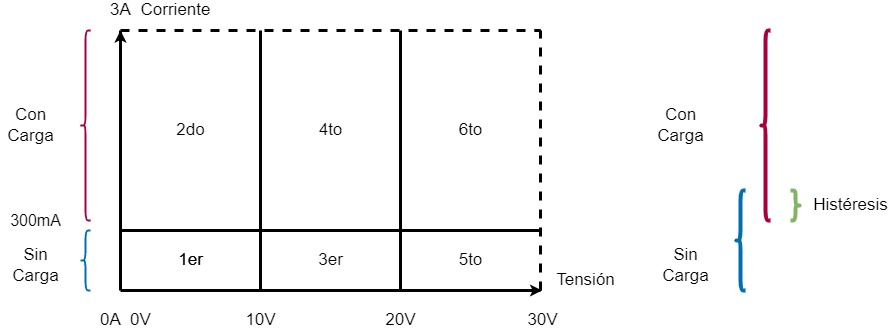
\includegraphics[width=1\textwidth]{./imagenes/matriz.jpg}
    \caption{Mapeo del rango de funcionamiento de la fuente.}
    \label{F:mapeo_cuadrantes}
\end{figure}\par

Un desafío de esta aproximación surge al acercarse a las zonas de transición entre las constantes del controlador, donde se produce un transitorio problemático en el cual el sistema podría perder estabilidad al cambiar de cuadrante. Para mitigar este inconveniente y asegurar que el controlador permanezca en el nuevo estado deseado, se desarrolló una ventana de histéresis como se ve en la parte derecha de la Figura \ref{F:mapeo_cuadrantes}. Esta ventana garantiza que la transición se complete de manera correcta, manteniendo la estabilidad del sistema en todo momento.\par


\subsection{Soft Reset}
Para evitar la confusión en el manejo de variables de control almacenadas en la memoria del dispositivo durante el funcionamiento, es fundamental mencionar la implementación de un \textit{soft reset} en el algoritmo de control. Este reinicio se encarga de restablecer todas las variables esenciales, como el error acumulado y el componente integrador, evitando que los valores previos influyan negativamente en el comportamiento del sistema cuando se pasa a un nuevo estado. El \textit{soft reset} permite que el sistema vuelva a un punto de referencia estable, similar al estado de reposo, garantizando así una respuesta controlada y óptima frente a nuevas condiciones de operación de la fuente, y previniendo posibles comportamientos indeseados como lo puede ser el aumento desmedido de la acción de control.\par


\subsection{Protección ante sobretensiones y falso contacto}
En sistemas electrónicos, es común que las cargas puedan tolerar valores de alimentación ligeramente inferiores al nominal durante unos pocos milisegundos hasta que la tensión se estabiliza. Sin embargo, esta tolerancia no se extiende a las sobretensiones, ya que incluso una sobretensión breve puede ser suficiente para dañar los componentes electrónicos de una carga. Por ello, la fuente de alimentación implementa un mecanismo de protección contra sobretensiones que desconecta de inmediato el relé de salida al detectar un valor de tensión superior al límite permitido. \par

Una vez eliminada la sobretensión y estabilizada la tensión de salida dentro de los límites predefinidos durante un tiempo determinado, el relé de salida se reactiva, permitiendo el acoplamiento seguro de la carga. Esta función es especialmente útil en casos de falso contacto, que pueden generar picos de tensión y perturbaciones en la salida de la fuente. Así, se proporciona una protección adicional a la carga, asegurando su integridad ante escenarios potencialmente dañinos. \par

Este mecanismo de protección no solo evita daños permanentes en los dispositivos conectados, sino que también garantiza una mayor durabilidad y fiabilidad del sistema en su conjunto, al reducir los riesgos asociados con fluctuaciones de tensión imprevistas. \par

\chapter{Interfaz de datos de entrada y salida}
% ----------------------

\label{C:Interfaz de datos de entrada y salida}

\section{Diagrama de bloques de la interfaz de datos}
Para la adquisición de las variables a controlar y el ingreso de datos de configuración por un lado, y para la visualización de variables y manejo del actuador de potencia, se propone el diagrama de bloques de la figura~\ref{F:diagrama_digital}. Se pretende controlar la tensión y corriente de salida en base al algoritmo de control del capitulo anterior que esta vinculado directamente con el ajuste de las referencias impuestas con un teclado numérico. A su vez, por el bus I2C se lleva a cabo la lectura de la tensión y de la corriente de salida mediante un convertidor AD de alta resolución de 16 bits mientras que los datos procesados se despliegan en un display OLED o LCD. En el display se visualiza la tensión y corriente de salida medidas, la tensión y corriente configurada deseada, y el modo de operación del sistema (CV o CI) así como también si la carga se encuentra conectada o desconectada entre otras funciones. Se agrega además, un comando de acople y desacople de la carga mediante el accionamiento de un relé.

\begin{figure} [H]
    \centering
    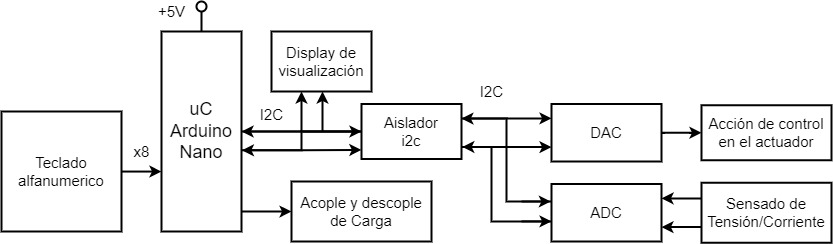
\includegraphics[scale=0.5]{./imagenes/diagrama_digital.jpg}
    \caption{Diagrama de bloques de la interfaz de datos.}
    \label{F:diagrama_digital}
\end{figure}

\section{Componentes de la etapa digital.}
Esta sección del informe está dedicada a desglosar y describir en detalle los componentes esenciales que constituyen la interfaz de manejo de datos de una fuente CC. La comprensión de cada componente, su función y su interacción con otros elementos es fundamental para diseñar un sistema confiable.\par 
Los componentes que se abordarán incluyen microcontroladores, convertidores analógico-digital (ADC), convertidores digital-analógico (DAC), sensores de corriente y voltaje, así como los circuitos de comunicación y control. Cada uno de estos elementos desempeña un rol específico y crítico en la gestión y monitoreo del suministro de energía. A través de esta sección, se explicarán las características técnicas de estos componentes, su importancia en el contexto del diseño de la fuente DC y cómo se integran para formar una unidad cohesiva y funcional.

\subsection{Microcontrolador Arduino Nano.}
El Arduino Nano es un microcontrolador compacto y versátil ampliamente reconocido por su facilidad de uso y sus diversas capacidades. Diseñado por Arduino LLC, este dispositivo ofrece un rendimiento sólido en un formato pequeño, lo que lo convierte en una opción popular para una amplia gama de aplicaciones en el ámbito de la electrónica amateur y profesional.\par 
Con su arquitectura avanzada y un conjunto completo de características, el Arduino Nano es ideal para proyectos que requieren control preciso y eficiente, así como para la interacción con diversos sensores y actuadores. Su capacidad para manejar operaciones en tiempo real lo hace adecuado para aplicaciones que van desde sistemas de automatización del hogar hasta dispositivos portátiles y gadgets interactivos.

\underline{Programación}: \par 
La programación del Arduino Nano se realiza utilizando el entorno de desarrollo integrado (IDE) de Arduino, que proporciona una interfaz intuitiva para escribir, cargar y depurar código. Compatible con una amplia variedad de bibliotecas y herramientas, el IDE de Arduino simplifica el proceso de desarrollo, permitiendo a los usuarios concentrarse en la lógica de su proyecto sin preocuparse por los detalles de bajo nivel del hardware.

\subsection{Teclado de membrana 4x4.}
El teclado de membrana matricial 4x4 autoadhesivo es un dispositivo de entrada que se utiliza comúnmente en aplicaciones electrónicas donde se requiere una interfaz de usuario simple y compacta. Consiste en una delgada lámina de material flexible que contiene una matriz de botones dispuestos en filas y columnas, con un total de 16 botones en este caso particular como se observa en la Figura \ref{F:teclado4x4} (4 filas x 4 columnas). \par 
Cada botón en el teclado de membrana está interconectado mediante una disposición de líneas conductoras en la membrana. Estas líneas están organizadas de manera que forman una matriz, permitiendo la detección de la ubicación específica de la tecla presionada. El funcionamiento del teclado de membrana matricial implica un proceso de escaneo continuo de todas las filas y columnas para detectar la presencia de un botón presionado. Cuando un botón se presiona, se cierra un circuito entre la fila y la columna correspondientes, lo que indica al microcontrolador la ubicación de la tecla activada.

\begin{figure}[H]
    \centering 
    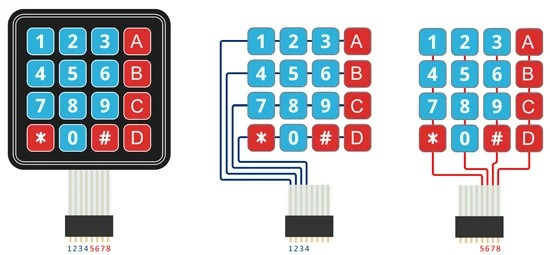
\includegraphics[scale=0.5]{./imagenes/Teclado Matricial 4x4_2.jpg}
    \caption{Ilustración del teclado de membrana, indicando sus filas y columnas.}
    \label{F:teclado4x4}
\end{figure}

\subsection{Display OLED SSD1306.}
El display OLED SSD1306 elegido para el proyecto utiliza comunicación I2C y ofrece una resolución de 128x64 píxeles. En la Figura \ref{F:display} se presenta una imagen del display, que opera dentro de un rango de voltaje de 3.3 a 5.5 V, lo cual lo hace compatible con el microcontrolador seleccionado. En esta pantalla se mostrará tanto el menú de funcionamiento, los modos de operación además de un indicador a tiempo real de las magnitudes registradas. Será el vínculo principal entre el usuario y la fuente.

\begin{figure}[H]
    \centering 
    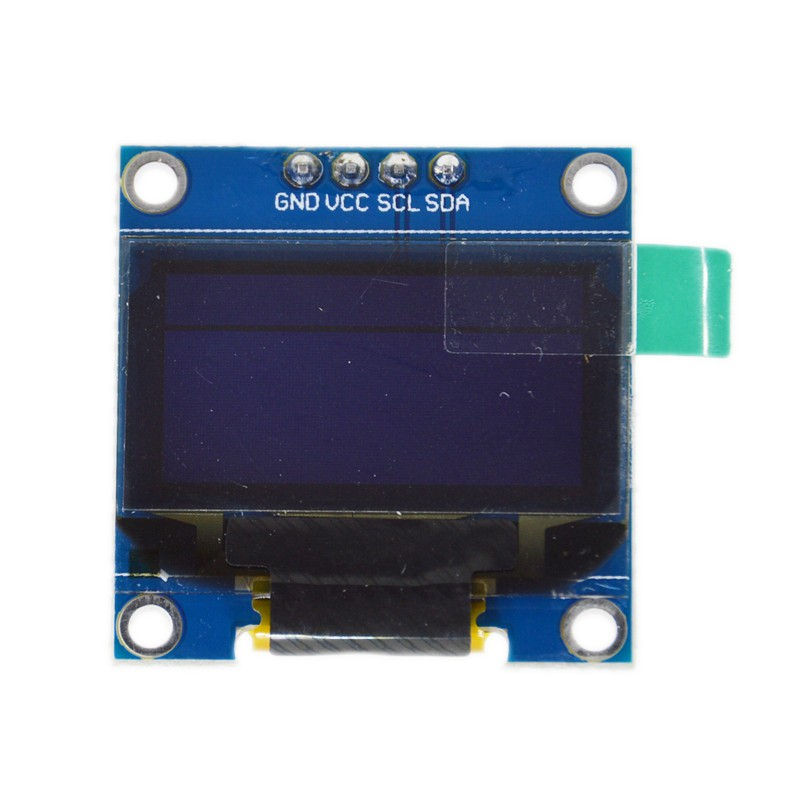
\includegraphics[scale=0.3]{./imagenes/display.jpg}
    \caption{Display OLED SSD1306.}
    \label{F:display}
\end{figure}

\subsection{Aislador I2C capacitivo.}
El dispositivo a utilizar es un ISO1540 \cite{ISO1540} el cual cuenta con buffers de entrada y salida que están separados por tecnología de aislamiento capacitivo de Texas Instruments que utiliza una barrera de dióxido de silicio (SiO2). Cuando se utilizan con fuentes de alimentación aisladas, estos dispositivos bloquean voltajes altos, aíslan tierras y evitan corrientes de ruido que puedan ingresar a la tierra local e interferir o dañar circuitos sensibles. Esta tecnología de aislamiento ofrece ventajas en función, rendimiento, tamaño y consumo de energía en comparación con los optoacopladores. \par 
De este modo tendremos la aislación galvánica para separar apropiadamente la parte de potencia de la de control.
\begin{figure}[H]
    \centering
    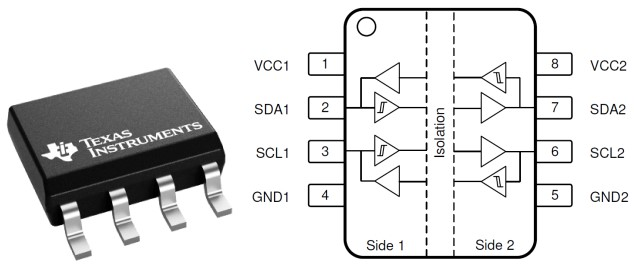
\includegraphics[scale=0.5]{./imagenes/optoi2c.jpg}
    \caption{Aislador capacitivo I2C ISO1540.}
    \label{F:optoi2c}
\end{figure}

\subsection{Convertidor analógico digital. ADC.}
El ADS1115 es un componente crucial en la transición de una fuente de alimentación de corriente continua de analógica a digital. Este dispositivo ofrece una impresionante precisión de 16 bits, junto con una velocidad de muestreo de hasta 860 muestras por segundo a través del protocolo de comunicación I2C. Configurable para operar con cuatro canales de entrada de un solo extremo o dos canales diferenciales, el ADS1115 se destaca por su versatilidad en la medición de señales analógicas en entornos digitales. \par 
Equipado con un conversor delta-sigma de 16 bits, un comparador programable con salida directa al pin de alerta, y una ganancia ajustable que permite la lectura de hasta 256mV en escala completa, este dispositivo garantiza una captura precisa de los datos analógicos. Su interfaz de comunicación I2C facilita la lectura de datos digitales, mientras que su dirección predeterminada de 0x48 y la disponibilidad de bibliotecas para plataformas como Arduino lo convierten en una opción conveniente y de fácil integración en proyectos electrónicos.
\begin{figure}[H]
    \centering
    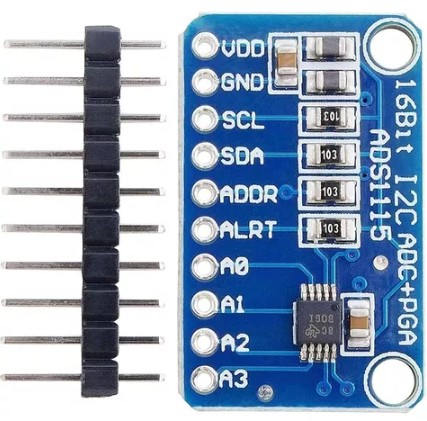
\includegraphics[scale=0.3]{./imagenes/ads1115.jpg}
    \caption{Convertidor AD ADS1115.}
    \label{F:ADC}
\end{figure}

\subsection{Convertidor digital analógico. DAC.}
El MCP4725 es un convertidor digital a analógico (DAC) que permite la conversión precisa de señales digitales en señales analógicas, lo cual es fundamental en aplicaciones donde se requiere una salida de voltaje analógico controlada digitalmente. Este dispositivo ofrece una resolución de 12 bits, proporcionando 4096 niveles de salida posibles y asegurando una alta precisión en la conversión de datos digitales.

Una característica destacada del MCP4725 es su interfaz de comunicación I2C, que permite una fácil integración con microcontroladores y otros dispositivos digitales. Además, incluye una memoria EEPROM interna que puede almacenar la configuración de salida, garantizando que el dispositivo mantenga su valor de salida incluso después de un reinicio.

El MCP4725 es particularmente útil en sistemas embebidos y de control, donde se necesita una conversión precisa y confiable de datos digitales a señales analógicas. Su pequeño tamaño y bajo consumo de energía lo hacen ideal para aplicaciones portátiles y de baja potencia.

\begin{figure}[H]
    \centering
    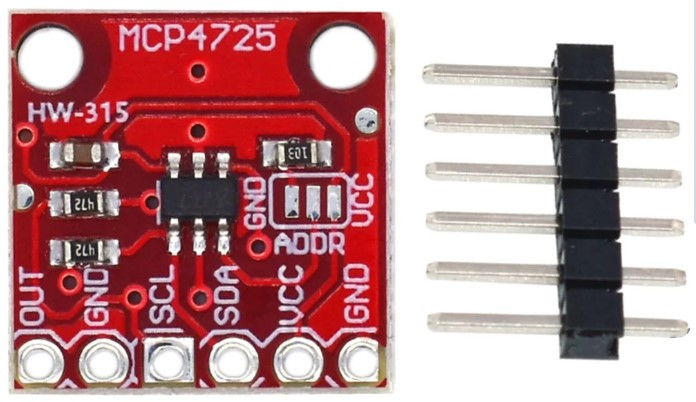
\includegraphics[scale=0.3]{./imagenes/mcp4725.jpg}
    \caption{Convertidor digital analógico MCP4725.}
    \label{F:DAC}
\end{figure}

\section{Modos de operación de la fuente.}
El sistema de control de la fuente de alimentación implementa varios modos de funcionamiento para adaptarse a diversas necesidades de aplicación. A continuación, se describen los principales modos de operación: \par 
\subsection{Modo Tensión}
En este modo, la fuente de alimentación establece inicialmente el valor máximo de tensión deseado. Posteriormente, limita la corriente máxima de umbral que la carga podrá obtener. Este modo es especialmente útil cuando se requiere controlar la tensión suministrada a la carga de manera precisa y garantizar la seguridad del sistema al limitar la corriente máxima.\par 
\subsection{Modo Corriente}
En el modo de corriente, la fuente de alimentación establece y controla la corriente suministrada a la carga. Este modo es útil en situaciones donde es crítico mantener la corriente dentro de ciertos límites para proteger los componentes de la carga y garantizar su correcto funcionamiento.\par 
\subsection{Modo Rampa}
El modo de rampa tiene como objetivo generar un aumento gradual y lineal de la tensión suministrada a la carga durante un período de tiempo determinado. Los parámetros configurables en este modo incluyen la tensión final deseada y el tiempo en el cual se alcanzará esta tensión desde un valor inicial de 0V. Este modo es útil en aplicaciones donde se requiere un inicio suave del sistema para evitar sobrecargas o picos de corriente al arrancar la carga.\par 

\input{contenido/7_software_y_diseño.tex}
\chapter{Modelado y construcción del PCB.}
% ----------------------

\label{C:EModelado y construcción del PCB.}

\section{Software y herramientas de diseño empleadas.}

A partir de los circuitos desarrollados en los capítulos anteriores, se procedió a diseñar una placa de circuito impreso (PCB) personalizada. Esta placa está diseñada para integrar todos los componentes necesarios y crear un prototipo funcional que permita realizar ensayos sobre materiales en una superficie comprimida. \par 
La modelación y diseño del PCB se llevaron a cabo utilizando el software KiCad, reconocido por su amplia gama de herramientas de personalización de componentes. Este software permite a los diseñadores lograr un alto nivel de precisión y calidad en sus diseños, adecuándose a las habilidades específicas de cada usuario.\cite{kicad} \par 
El proceso de diseño incluyó la disposición estratégica de los componentes para optimizar el rendimiento del circuito, así como la consideración de factores como la disipación de calor, la integridad de la señal y la minimización de interferencias electromagnéticas. Además, se realizaron varias iteraciones del diseño para asegurar que el PCB final cumpliera con todos los requisitos técnicos y de funcionamiento necesarios para los ensayos planificados. \par 
El uso de KiCad facilitó la creación de un diseño detallado y eficiente, permitiendo visualizar en todo momento el aspecto final del PCB y realizar ajustes necesarios antes de proceder a su fabricación.

\section{Construcción del primer prototipo.}
La fase de construcción se inició con el desmontaje de la placa analógica de la fuente utilizada en un proyecto anterior que se puede apreciar en la Figura \ref{F:placa_original}, la cual se caracterizaba por sus atributos de control predominantemente analógicos. Este proceso permitió la recuperación de una variedad de materiales que, en su mayoría, se emplearían en el desarrollo del nuevo prototipo de fuente digital. Entre los componentes rescatados se encuentran resistencias, capacitores, disipadores de calor, borneras, entre otros. La reutilización de estos elementos fue posible gracias a la topología de la nueva fuente digital, que permitía su integración sin comprometer el diseño ni la funcionalidad del prototipo.  \par 
El proceso de desmontaje y reutilización de componentes se llevó a cabo meticulosamente, asegurando que cada pieza recuperada estuviera en condiciones óptimas para su reimplementación como se observa en la Figura \ref{F:desmontaje_de_la_placa}. Este esfuerzo contribuyó a la eficiencia del proyecto y a la racionalización de recursos, destacando la importancia de la sostenibilidad y la economía circular en el ámbito del diseño y construcción de dispositivos electrónicos.
\begin{figure}[H]
    \centering
    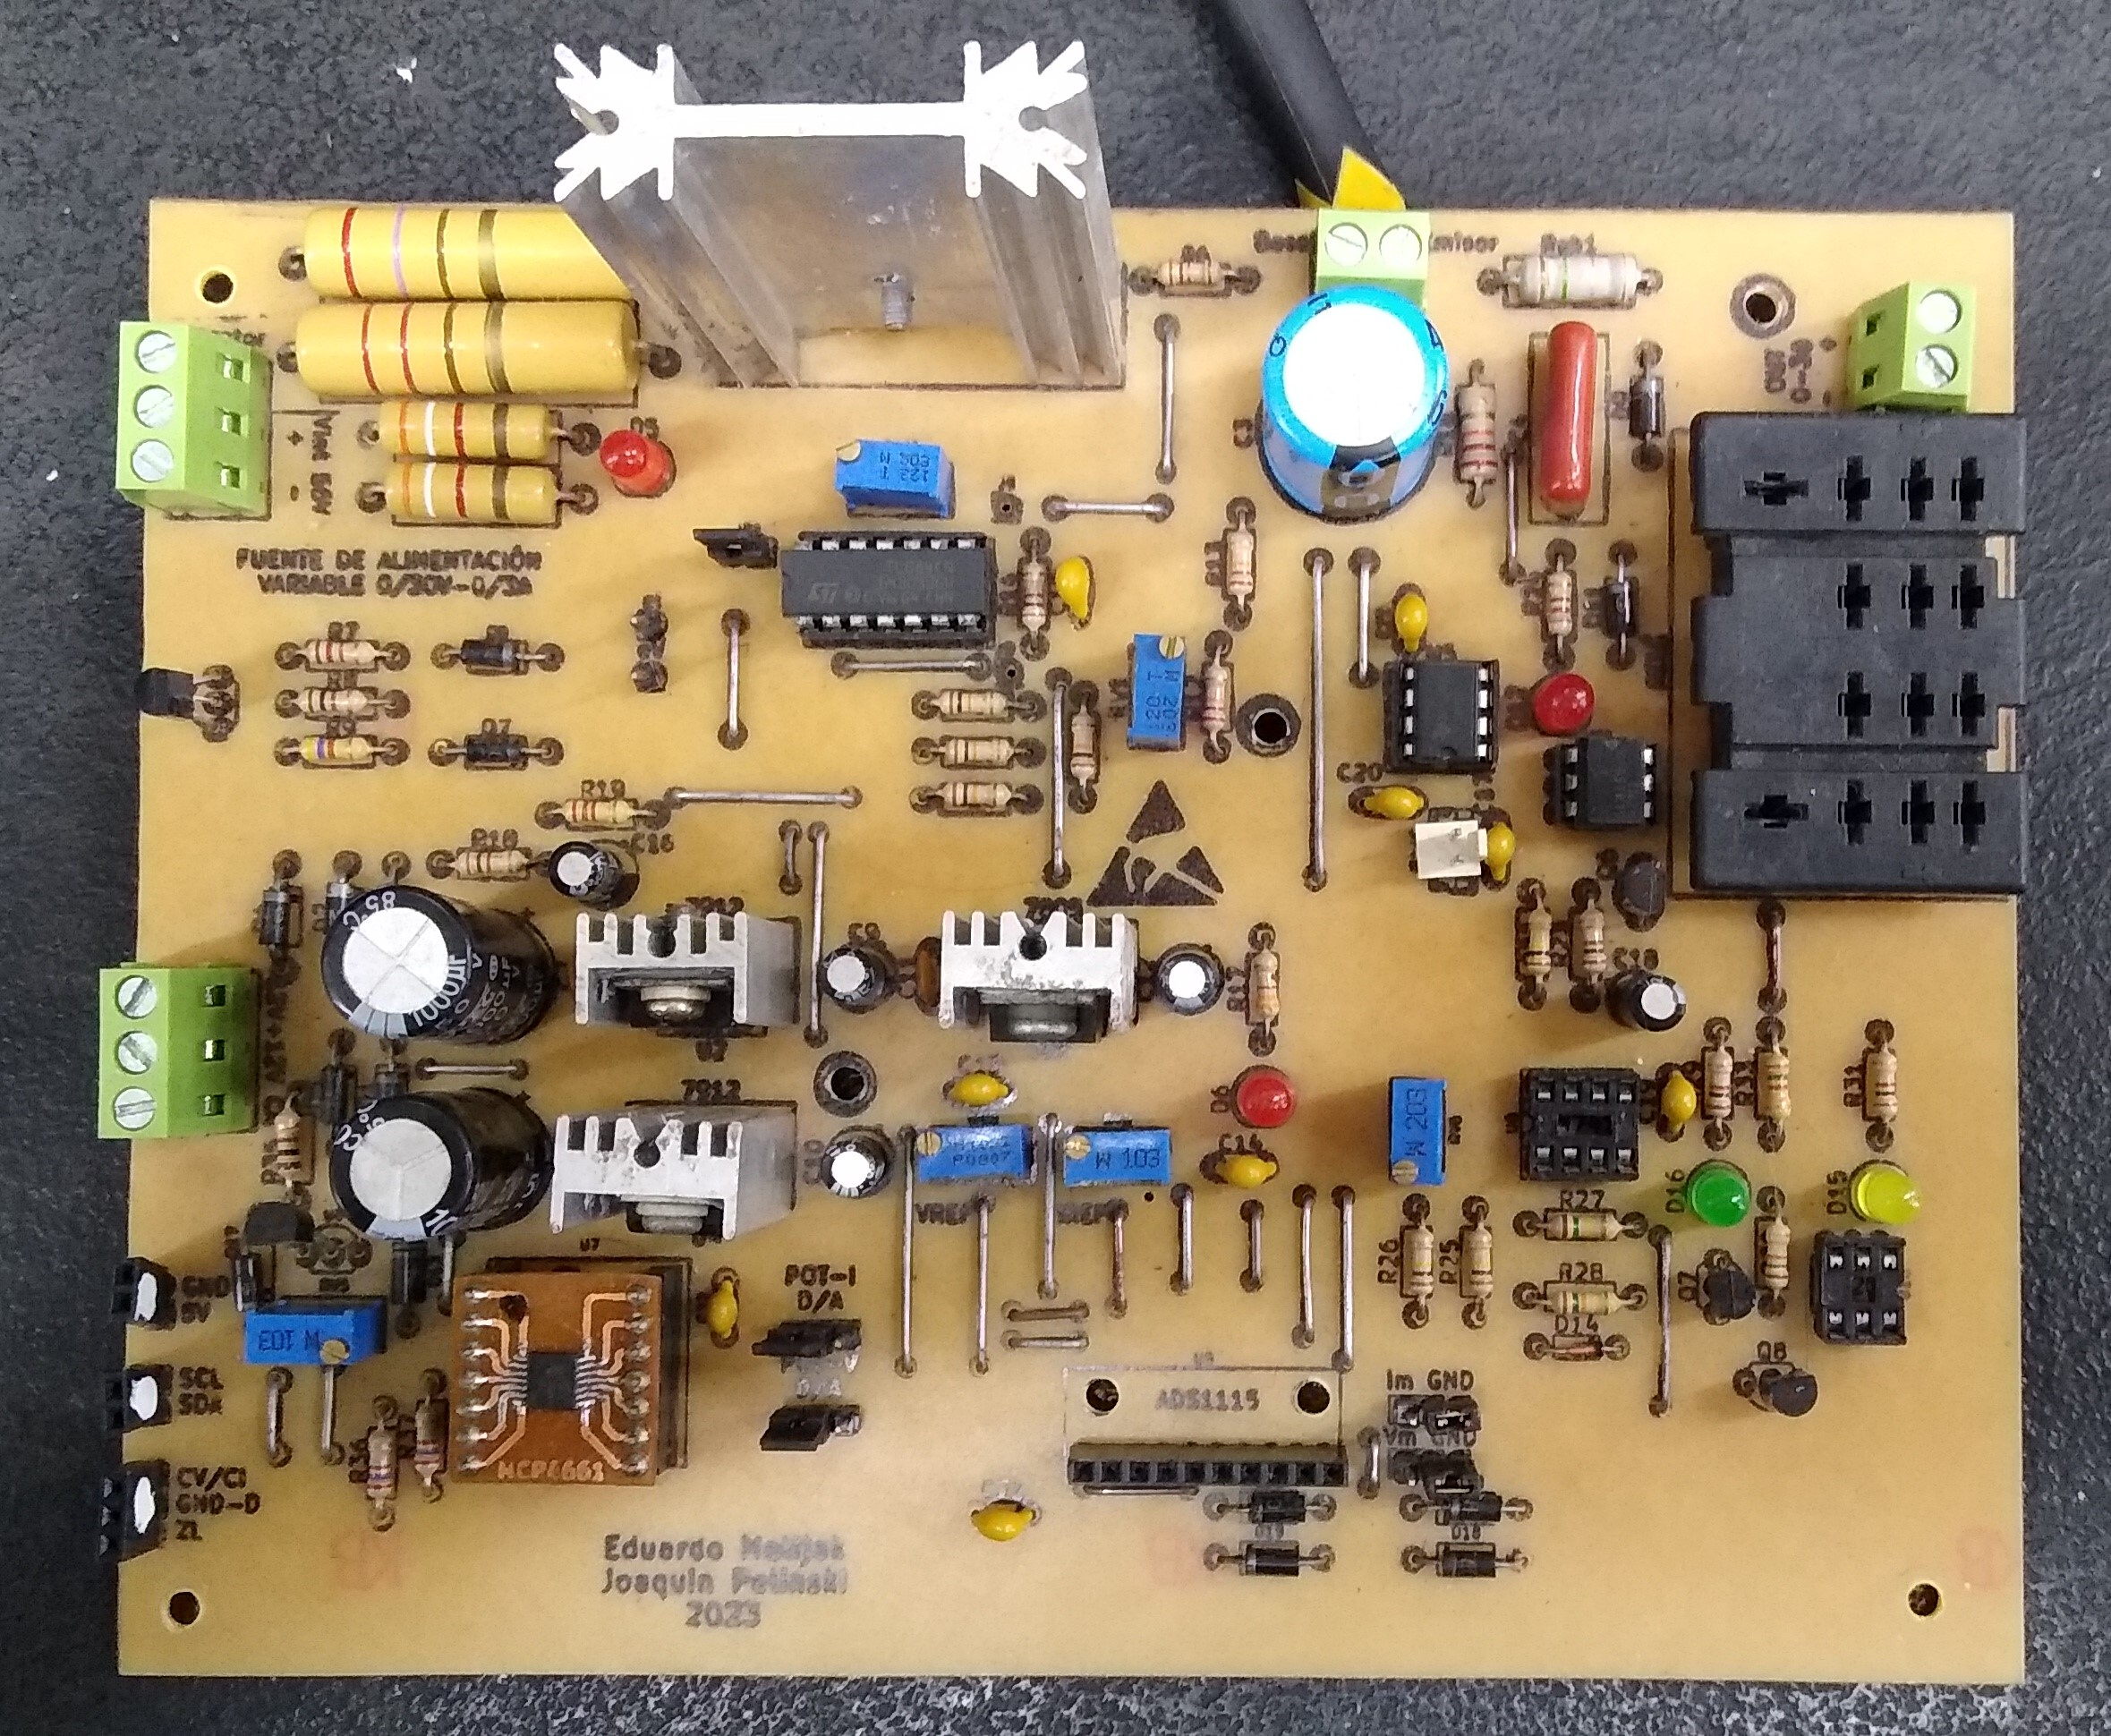
\includegraphics[width=0.8\textwidth]{./imagenes/fotos/placa_original.jpg}
    \caption{Antes del desmontaje de la placa de control analógica.}
    \label{F:placa_original}
\end{figure}

\begin{figure}[H]
    \centering
    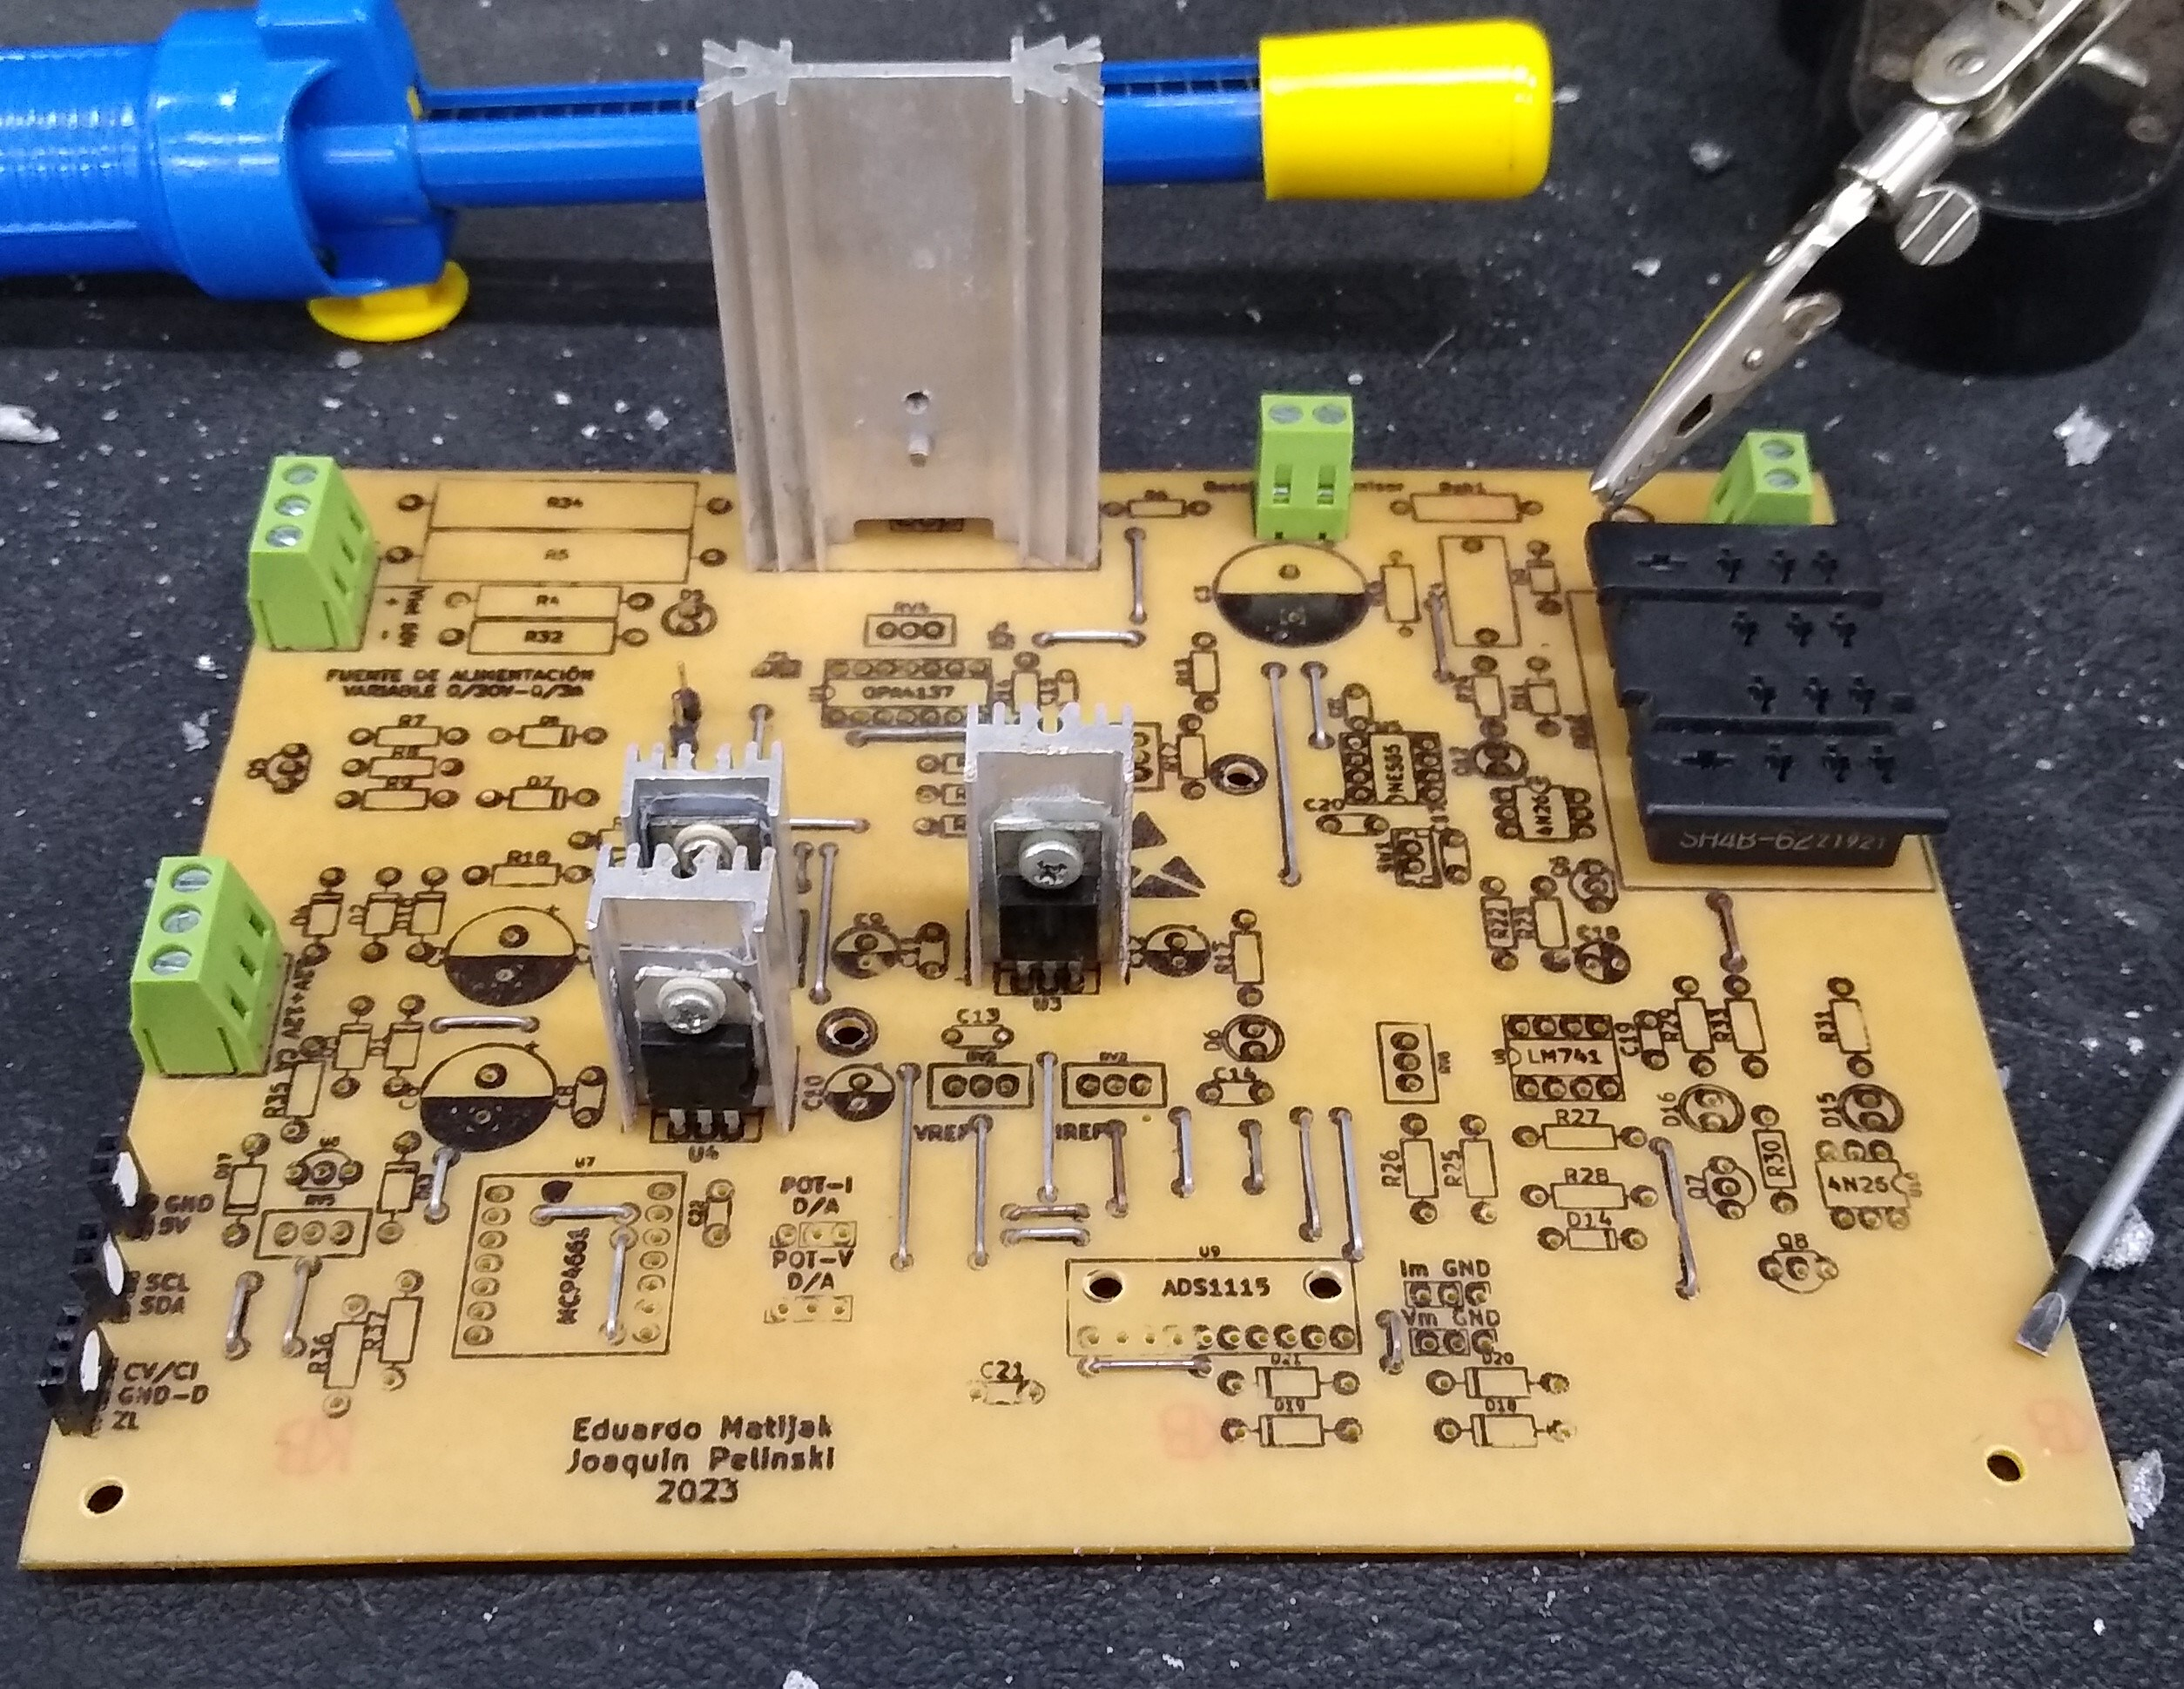
\includegraphics[width=0.8\textwidth]{./imagenes/fotos/desmontada.jpg}
    \caption{Después del desmontaje de la placa de control analógica.}
    \label{F:desmontaje_de_la_placa}
\end{figure}\par 
A continuación, se presenta el diseño del prototipo utilizado, el cual incorpora todos los elementos necesarios para la realización de las pruebas de funcionamiento. La característica principal de este PCB es su capacidad para integrar en un espacio compacto de 15x20 cm todos los componentes que anteriormente estaban dispersos en el modelo anterior. \par 
Una excepción notable en el diseño es la ubicación de la pantalla y el teclado, que se ha decidido mantener separados del PCB principal. Esta decisión se tomó debido a que no tendría sentido práctico incluir estos elementos directamente sobre la placa. En su lugar, se emplearon pines de salida, como borneras, para conectar estos componentes externos, facilitando su integración y operación. \par 
El diseño resultante, que se muestra en la Figura \ref{F:PCB_V1}, incluye también una representación tentativa en 3D del PCB. En esta representación se pueden observar las disposiciones de los componentes y la estructura general del prototipo. Es importante destacar que, para evitar daños y facilitar el acceso y reemplazo, algunos de los componentes están montados sobre tiras de pines hembra en lugar de estar soldados directamente sobre la placa. Esta configuración no solo mejora la durabilidad del prototipo, sino que también permite una mayor flexibilidad en la realización de pruebas y modificaciones. 
\begin{figure}[H]
    \centering
    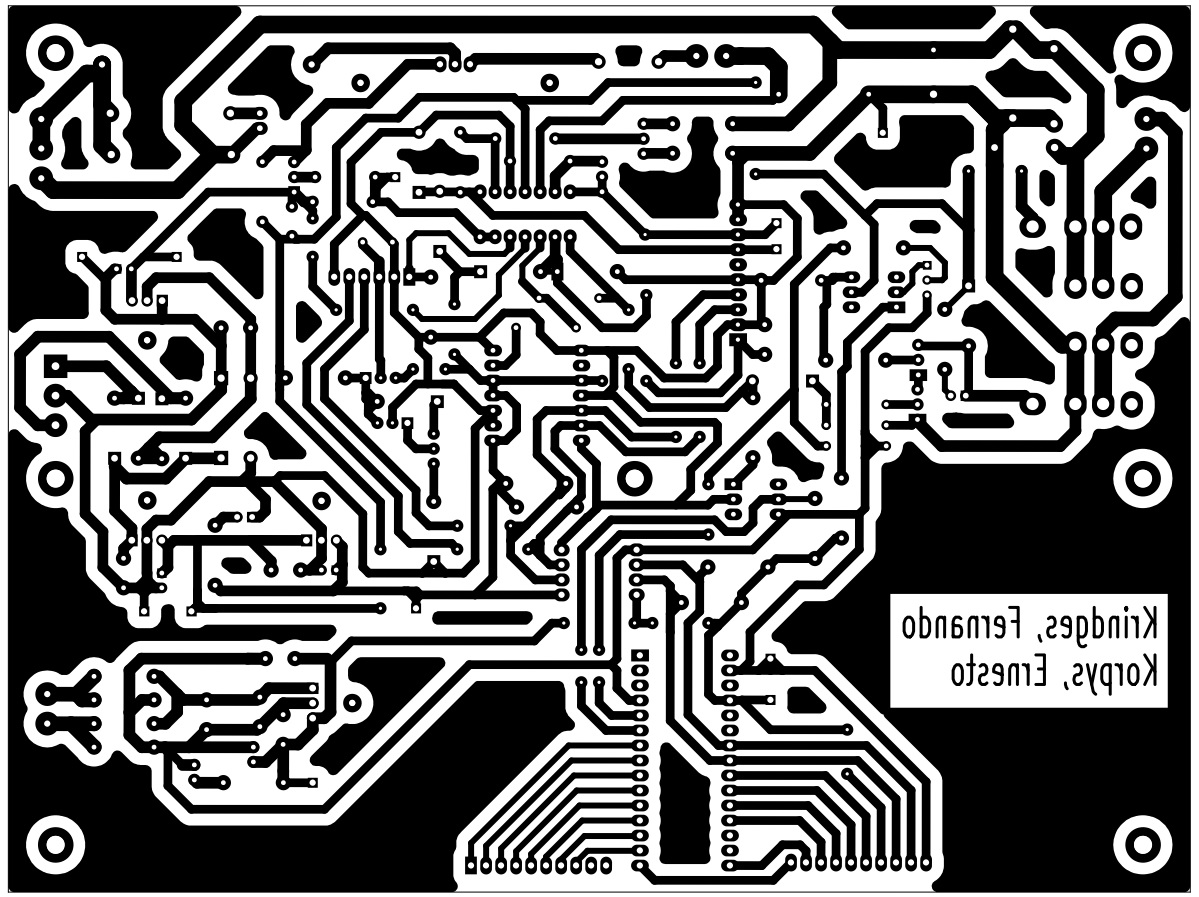
\includegraphics[width=\textwidth]{./imagenes/pcb_v1.jpg}
    \caption{Primer prototipo de PCB.}
    \label{F:PCB_V1}
\end{figure}
Se incluye un modelo 3D en el diseño con el fin de visualizar la disposición y la accesibilidad de los componentes, asegurando que el montaje y el mantenimiento del PCB sean lo más eficientes posible. Este es presentado en la Figura \ref{F:PCB_3D}.
\begin{figure}[H]
    \centering
    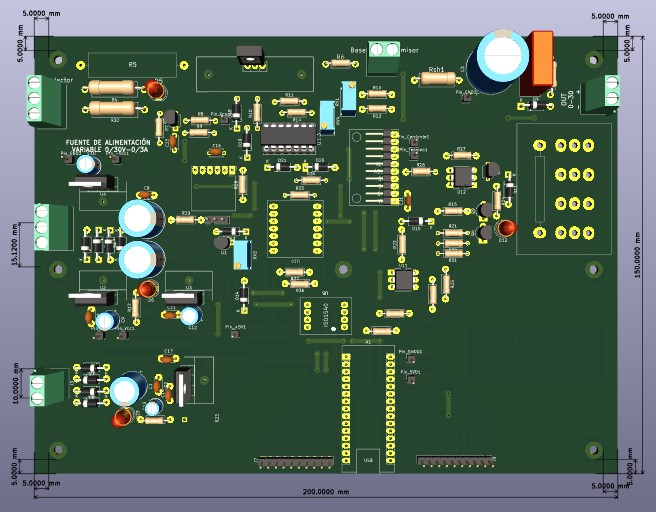
\includegraphics[width=\textwidth]{./imagenes/prototipo1.jpg}
    \caption{Vista 3D del primer prototipo.}
    \label{F:PCB_3D}
\end{figure} \par 
\begin{figure}[H]
    \centering
    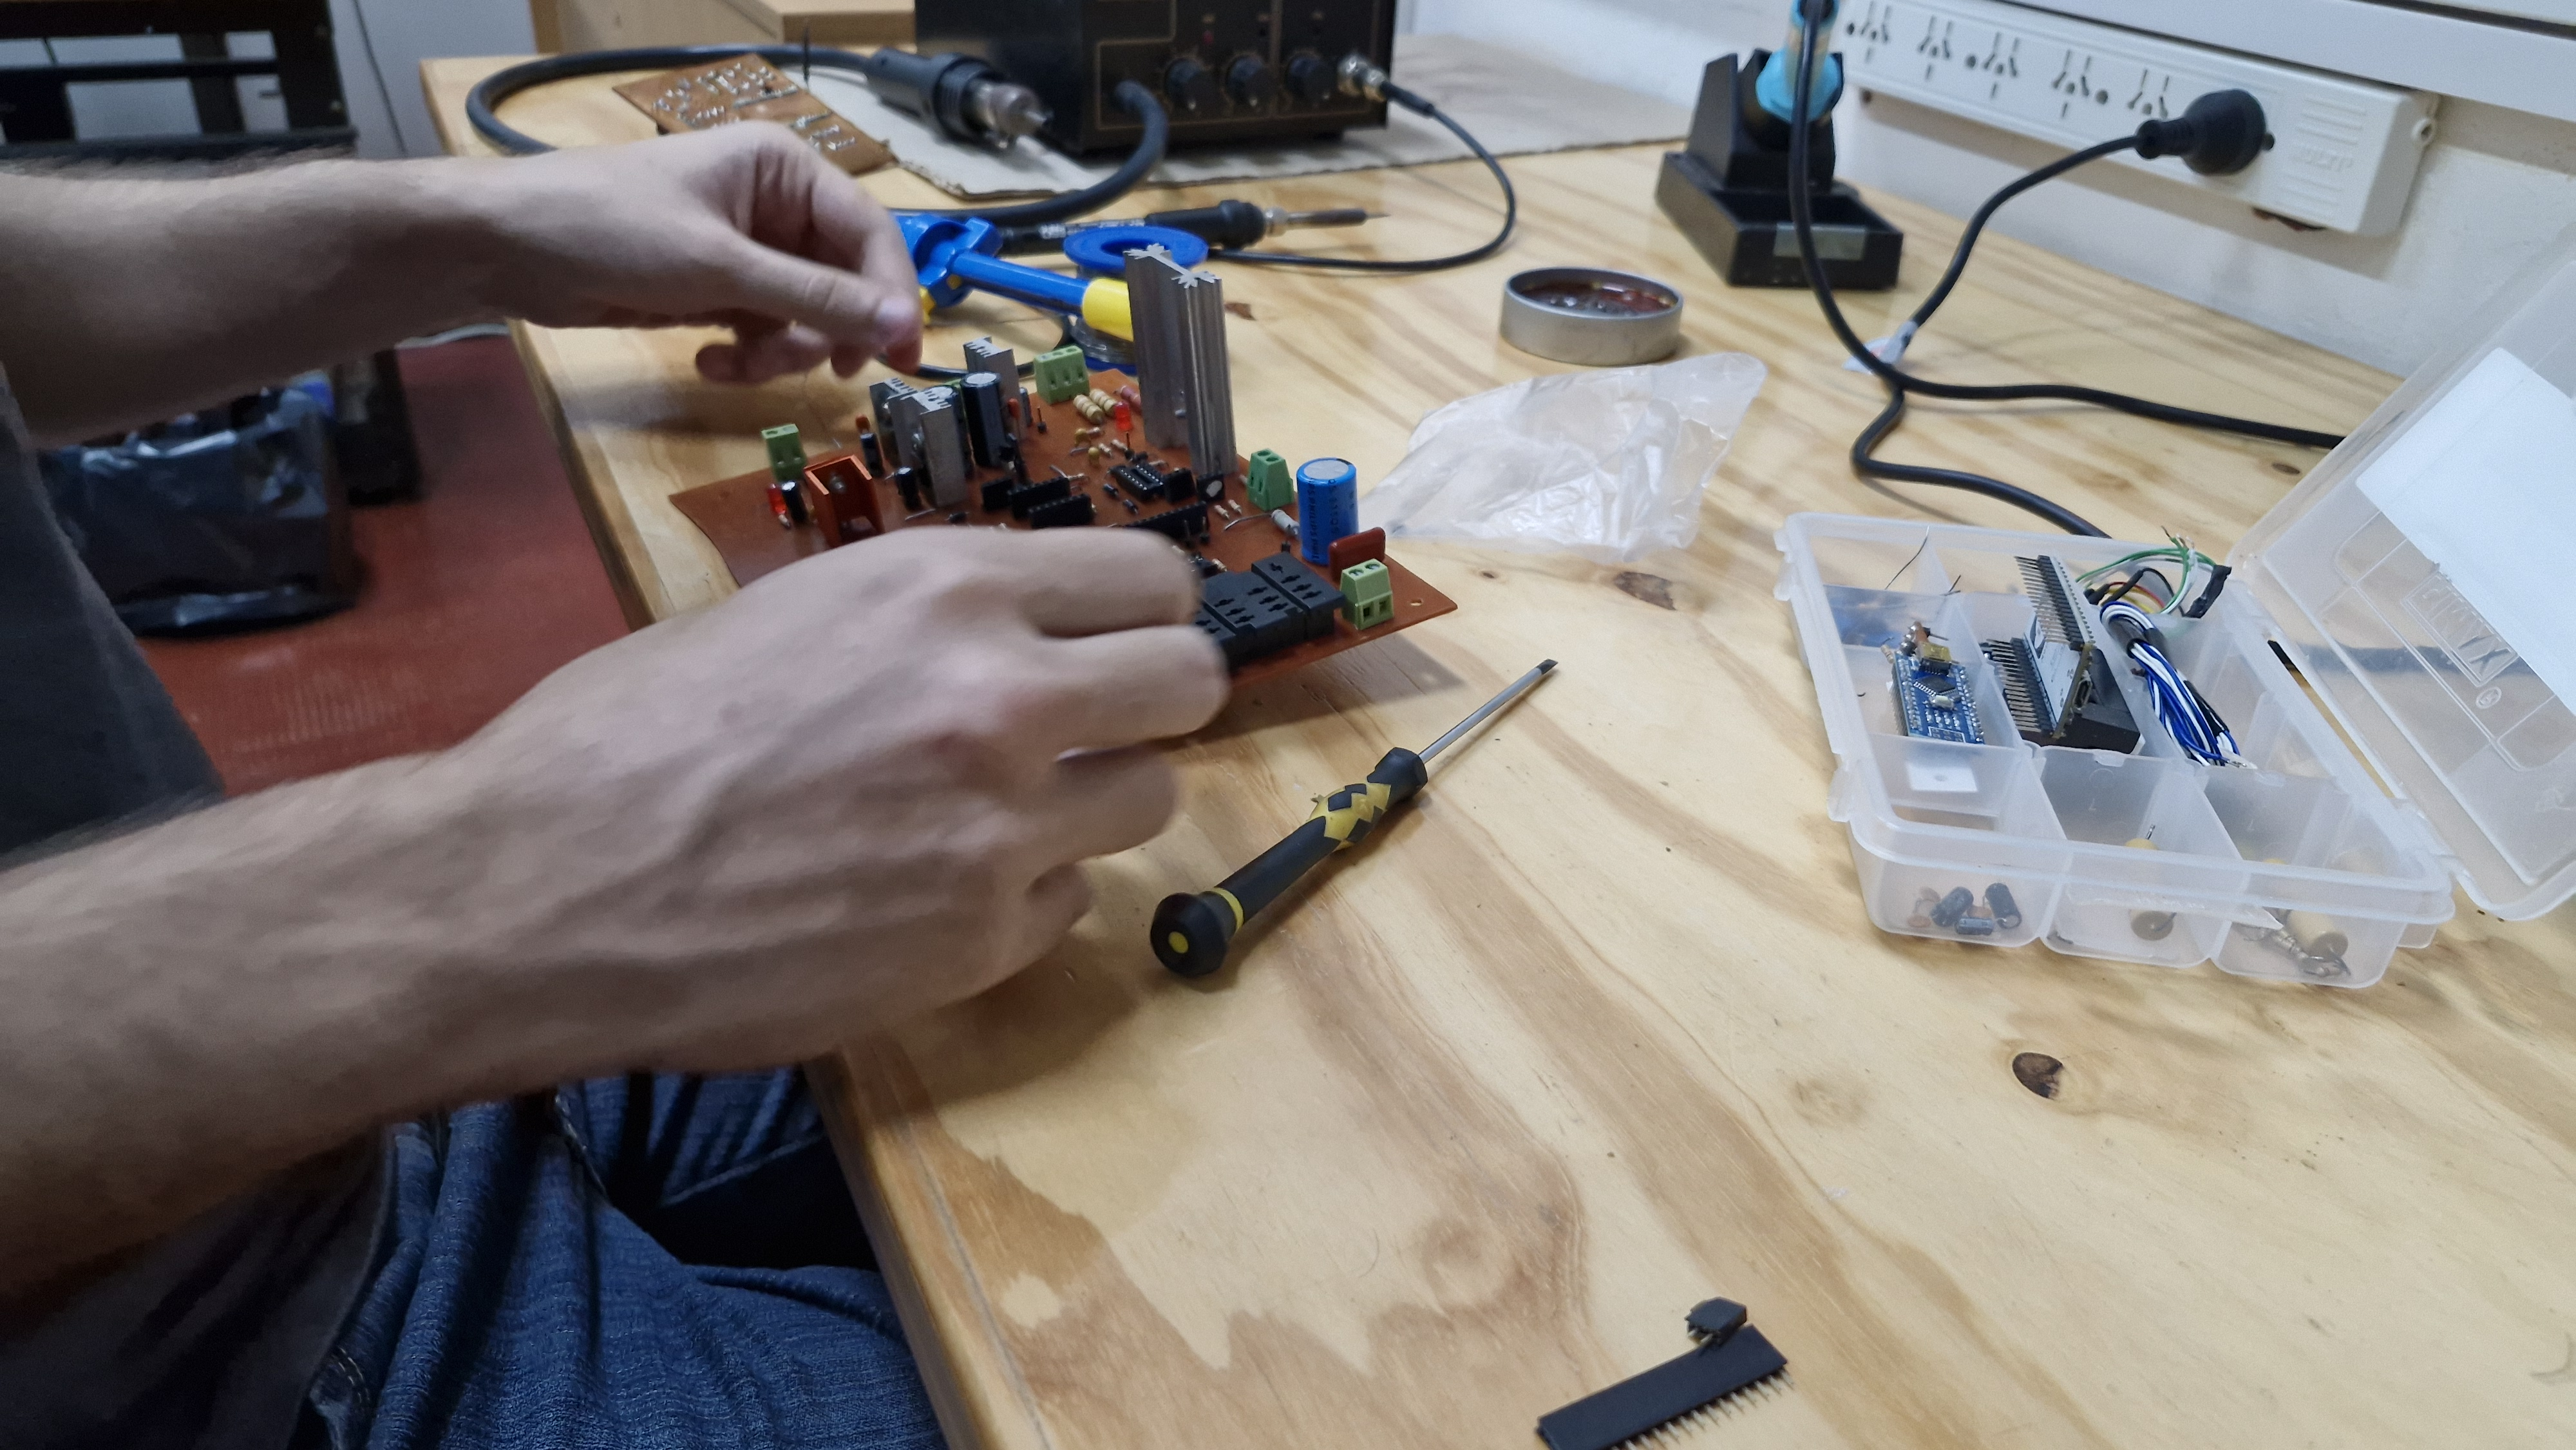
\includegraphics[width=\textwidth]{./imagenes/fotos/montaje.jpg}
    \caption{Montaje de los componentes en la placa.}
    \label{F:montaje_componentes}
\end{figure} \par 

\section{Ensayo de laboratorio y pruebas prácticas.}
Una vez verificada la continuidad de las pistas, el adecuado funcionamiento de los componentes, y los niveles de tensión en varios puntos clave, se procedió a energizar la fuente con todos los transformadores, tomando todas las precauciones necesarias para evitar daños a los componentes.\par 
A partir de este punto, se realizó una serie de pruebas y ajustes detallados para garantizar el correcto funcionamiento de la fuente. Estas pruebas incluyen la verificación de la respuesta del sistema bajo diversas condiciones de carga y la evaluación de la estabilidad del lazo de control. El uso del osciloscopio fue fundamental en este proceso, como se aprecia en la Figura \ref{F:esayos_y_pruebas}, ya que permitió observar en tiempo real cómo el lazo de control afectaba la salida de la fuente, aspecto crucial para el correcto desempeño del dispositivo.
Durante estas pruebas, se monitorizaron diversos parámetros, tales como la tensión de salida, la respuesta transitoria, y el comportamiento ante variaciones en la carga. Cada ajuste se realizó con el objetivo de optimizar la \textit{performance} del prototipo, asegurando que este cumpliera con los requisitos especificados y operara de manera eficiente y estable.\par 

\begin{figure}[H]
    \centering
    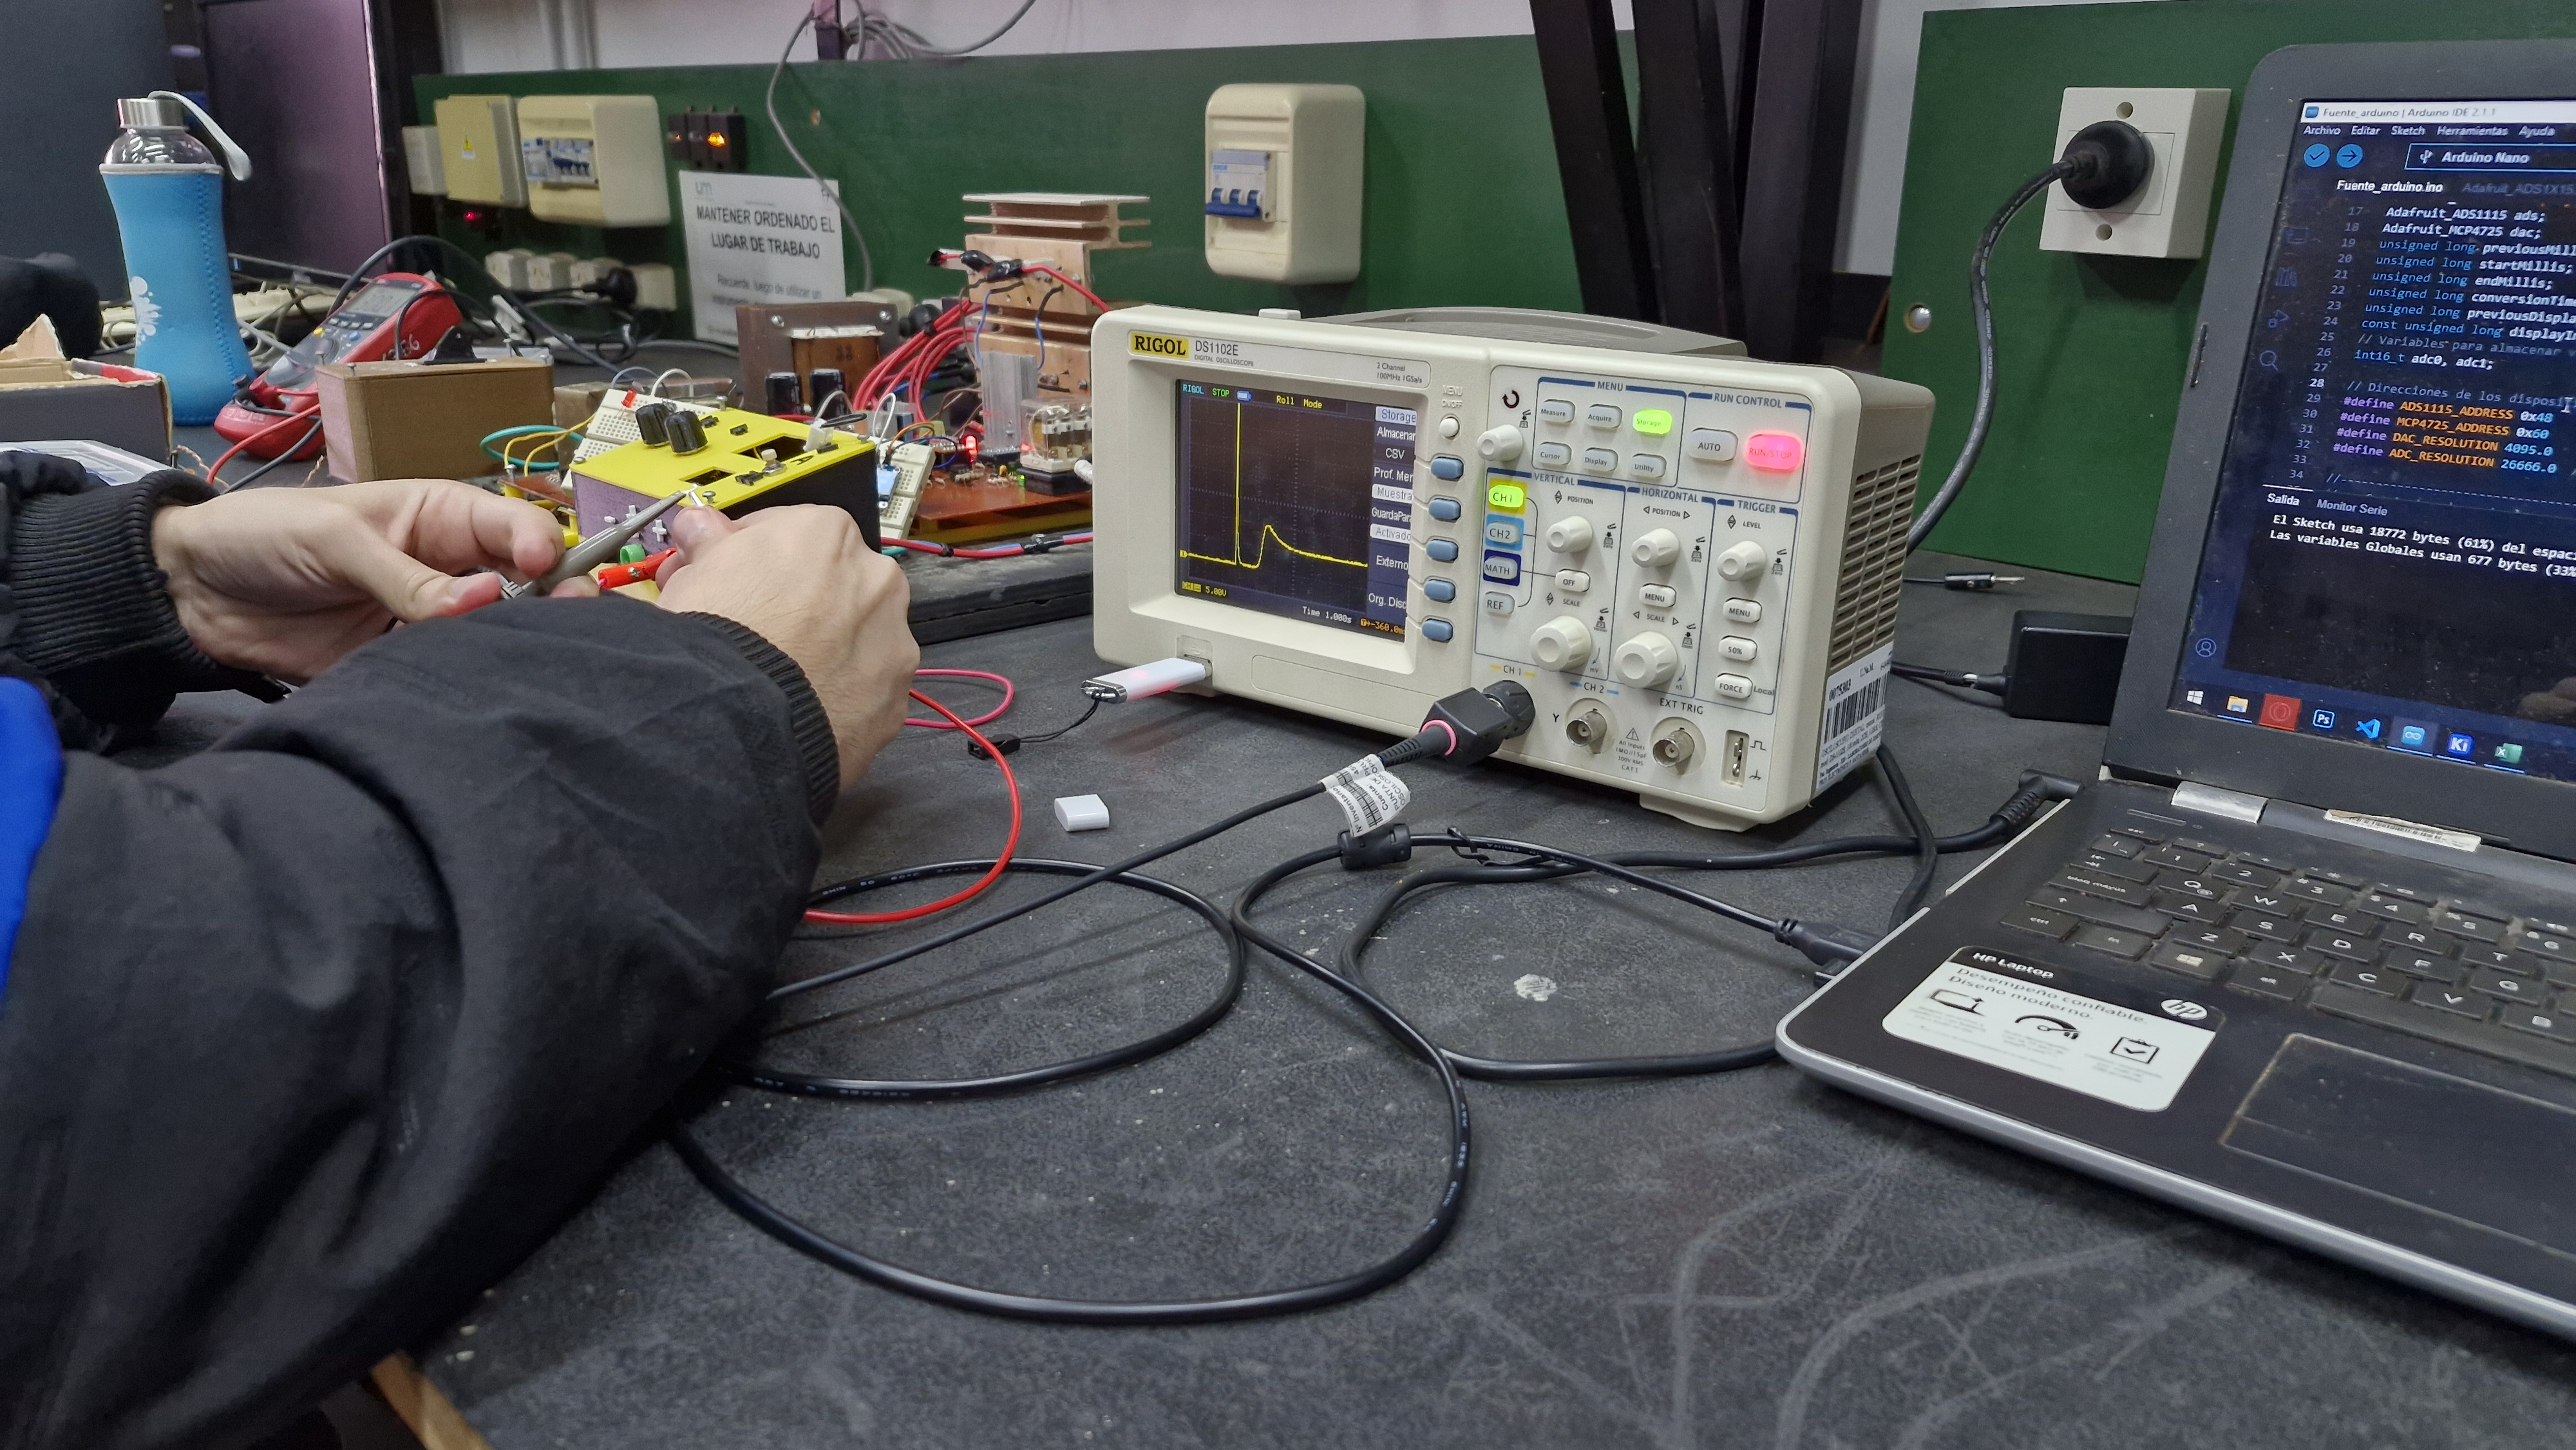
\includegraphics[width=0.9\textwidth]{./imagenes/fotos/osciloscopio.jpg}
    \caption{Ensayo con osciloscopio de la placa.}
    \label{F:esayos_y_pruebas}
\end{figure}
El resultado de estos ensayos fue satisfactorio, evidenciando que el diseño y la construcción del PCB fueron exitosos pero sin embargo no del todo concluyentes. Por lo que para la construcción del siguiente prototipo, se obtuvieron las siguientes observaciones que serán tomadas en cuenta.  \par 
\section*{Observaciones}
\begin{itemize}
    \item Los transistores comienzan a operar con una acción de control mínima de $0,3V$.
    \item Ante condición de vacío el capacitor de salida se carga y dispara su voltaje en cuestión de unos milisegundos, por lo que es necesario un control especial para contemplar este detalle.
    \item Cuando el DAC se inicializa establece su voltaje de salida en $2,5V$. Luego de analizar su hoja de datos, es posible escribir en su memoria EEPROM el valor por defecto con el cual iniciará.
    \item Hubo un error en la asignación de la huella del DAC, teniendo dos de sus pines invertidos entre sí.
\end{itemize}

\section*{Mejoras a realizar}
\begin{itemize}
    \item Ajuste de constantes de controlador.
    \item Ajuste de frecuencia de muestreo.
    \item Mejora de la estrategia de control.
    \item Arreglar la huella y el \textit{ruteo} de las pistas relacionadas al DAC.
\end{itemize}


\chapter{Segundo prototipo.}
% ----------------------

\label{C:Construcción de modelo final}

\section{Construcción de la fuente definitiva}

A partir de la experiencia obtenida en el desarrollo y las pruebas del primer prototipo de la fuente de tensión, se identificaron varios errores en las huellas y pistas del PCB. Estos problemas fueron corregidos en una nueva versión del diseño, abordando específicamente las fallas detectadas en la etapa inicial. Cada ajuste realizado fue producto de un análisis detallado de las fallas observadas, lo que permitió aprender de los errores y aplicar mejoras sustanciales en esta segunda iteración.\par 
Con esta evolución del diseño, se ha alcanzado el modelo definitivo dentro del marco de este proyecto, logrando cumplir con todos los objetivos planteados desde el inicio. Las funcionalidades establecidas, junto con las mejoras integradas, permiten asegurar que este prototipo final es una solución efectiva y alineada con los parámetros establecidos en la planificación original.\par

\section{Presentación Física.}
Uno de los aspectos distintivos que se abordó en esta versión final de la fuente de alimentación es la optimización de su presentación. El modelo anterior presentado en la figura \ref{F:fuente_anterior} carecía de un diseño compacto y organizado que integrara todos los componentes en un espacio reducido y controlado. Esta carencia no solo dificultaba el traslado del equipo, sino que también exponía sus partes a posibles daños causados por factores ambientales, como humedad, polvo o cambios de temperatura, que podrían afectar negativamente su funcionamiento a largo plazo.\par
Se dio especial atención al desarrollo de un diseño que no solo cumpliera con las especificaciones técnicas y funcionales, sino que también ofreciera una presentación estética y práctica. La disposición interna de los componentes fue planificada para maximizar el uso del espacio disponible, permitiendo una configuración más ordenada y accesible. Además, el gabinete contenedor seleccionado provee una protección robusta contra las condiciones ambientales adversas, asegurando que todos los elementos estén resguardados y puedan operar de manera óptima incluso en entornos desafiantes.\par

\begin{figure}[H]
    \centering
    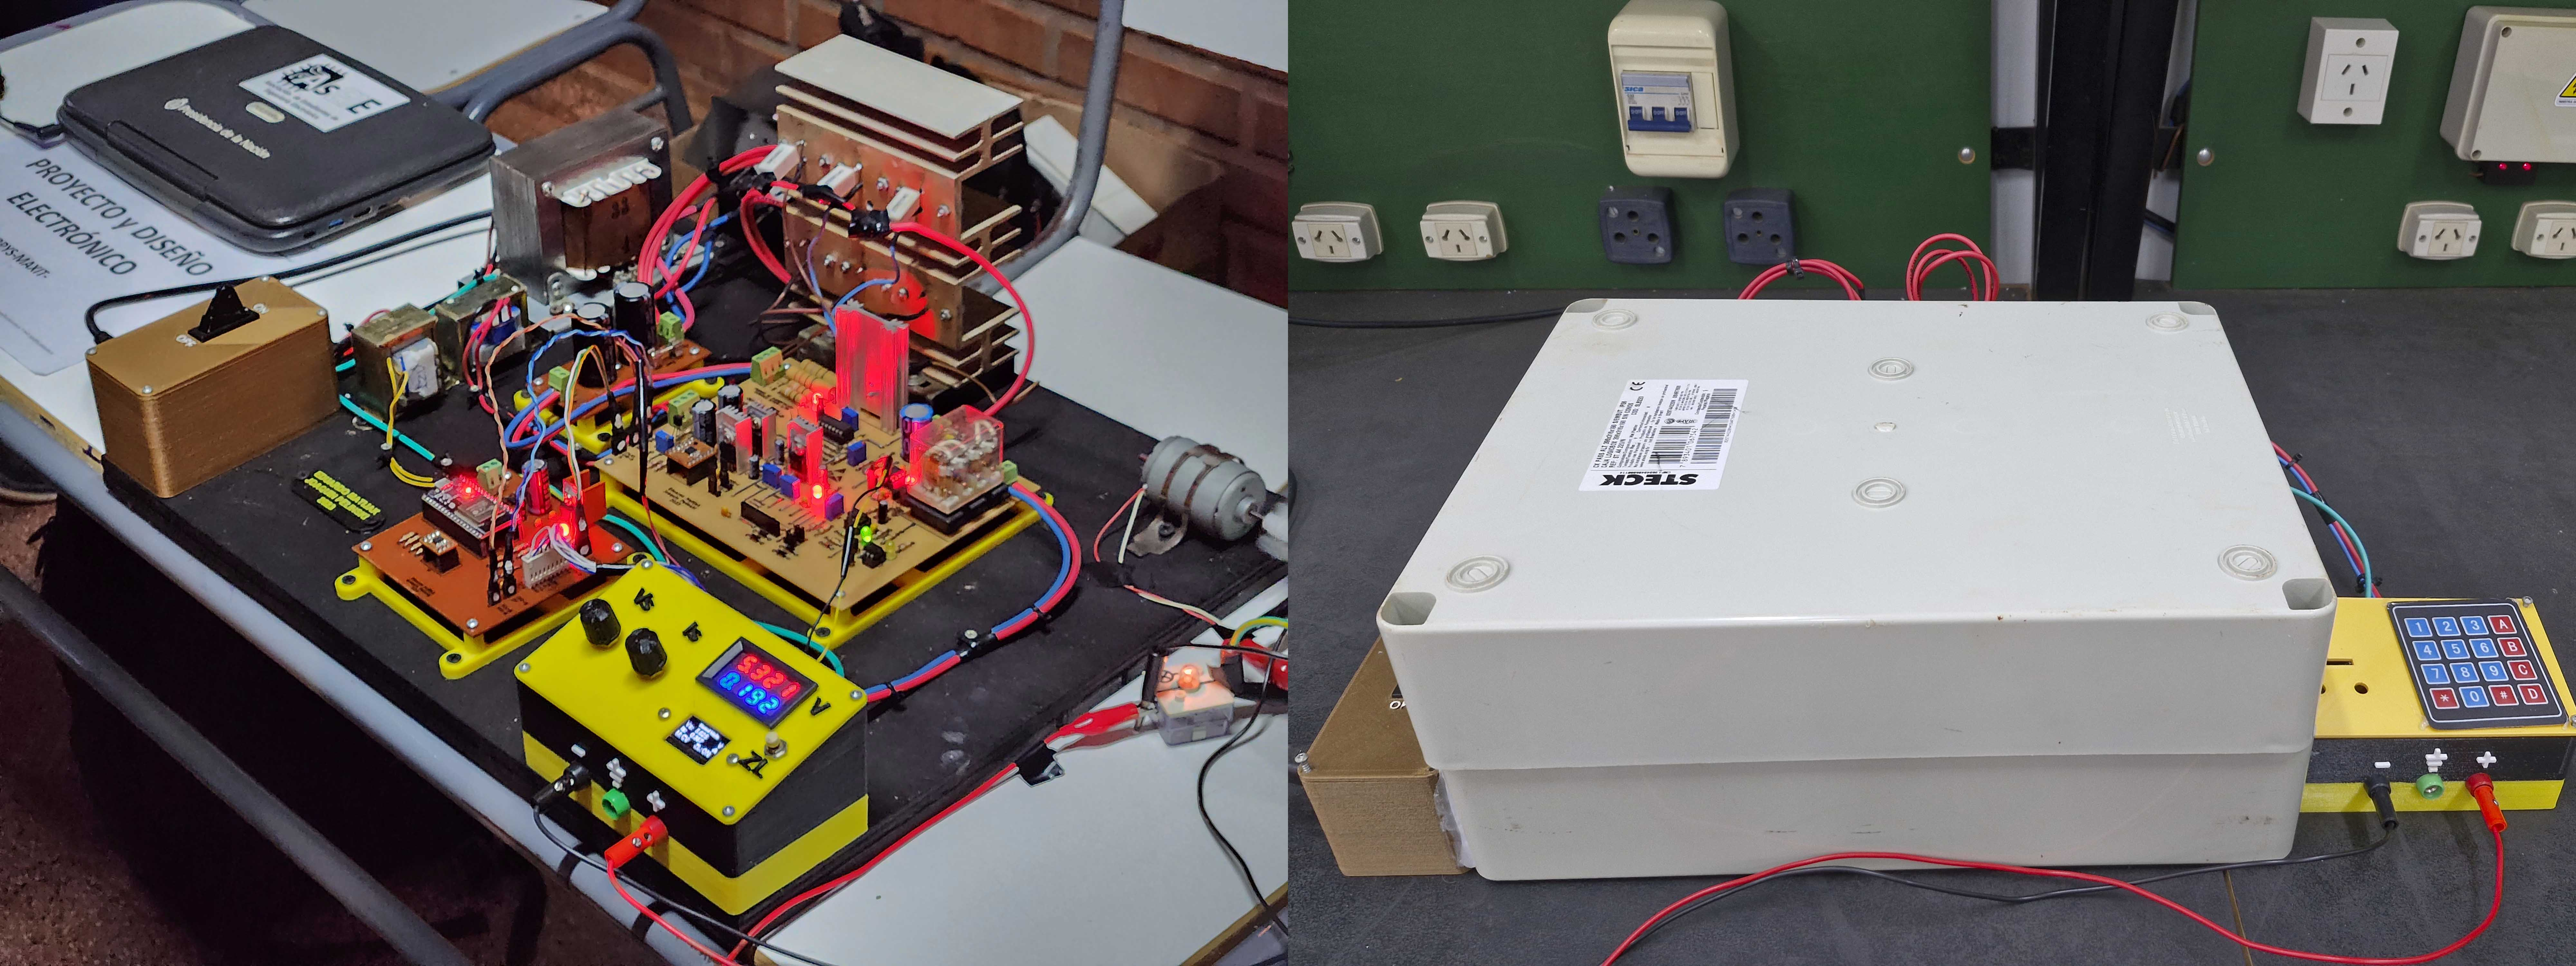
\includegraphics[scale=0.05]{./imagenes/fuente_anterior.jpg}
    \caption{Antes y después de realizada la modernización de la fuente.}
    \label{F:fuente_anterior}
\end{figure}

\subsection{Gabinete contenedor.}
Para la protección y organización de los componentes de la fuente de alimentación, se seleccionó una caja plástica de grandes dimensiones, la cual ofrece tanto espacio adecuado como resistencia estructural. Este gabinete, identificado en la figura \ref{F:gabinete_contenedor}, proporciona una contención segura para la mayoría de los elementos críticos del sistema. En su diseño, se ha dejado espacio en el exterior para el montaje de la pantalla y los controles de configuración, lo que facilita su acceso y manipulación por parte del usuario. Además, el disipador de calor fue montado externamente para optimizar la ventilación y la disipación térmica.\par
Las distintas secciones de la fuente fueron ubicadas estratégicamente, con el objetivo de maximizar el uso eficiente del espacio disponible en el gabinete contenedor, como se muestra en la figura \ref{F:distibucion_gabinete_contenedor}. Se priorizó una disposición organizada y armónica de los componentes y conductores, minimizando el desorden y asegurando una separación adecuada para evitar interferencias o cruces innecesarios entre las conexiones eléctricas.

\begin{figure}[H]
    \centering
    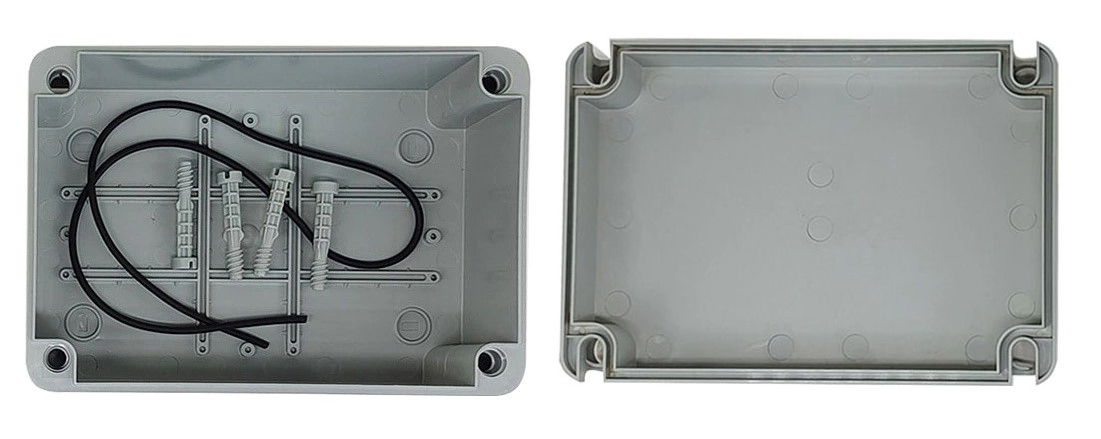
\includegraphics[width=0.8\textwidth]{./imagenes/caja_plastica.jpg}
    \caption{Caja plástica grande - 220×150×90 mm.}
    \label{F:gabinete_contenedor}
\end{figure}

\begin{figure}[H]
    \centering
    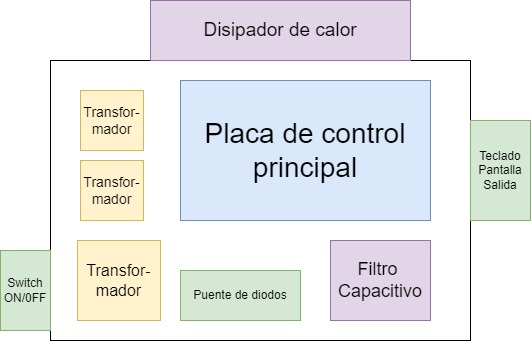
\includegraphics[scale=0.5]{./imagenes/distribucion_secciones.jpg}
    \caption{Distribución de secciones en el gabinete contenedor.}
    \label{F:distibucion_gabinete_contenedor}
\end{figure}

\subsection{Superficie de Montaje Interna}
Para asegurar una base estable y duradera para los componentes electrónicos, se optó por el uso de una superficie de madera forrada, evitando así el montaje directo sobre la caja plástica. Esta solución no solo proporciona una mayor firmeza al atornillar las piezas, sino que también facilita la organización interna y el acceso a los componentes cuando sea necesario realizar ajustes o mantenimientos.\par
La base de madera fue cuidadosamente fijada al fondo del gabinete otorgando bastante estabilidad. Para mejorar aún más la seguridad y la disposición de los circuitos, se diseñaron y fabricaron soportes plásticos mediante impresión 3D como se ve en la figura \ref{F:base3d_fuente}. Estos soportes fueron especialmente diseñados para mantener las placas electrónicas en posición suspendida, evitando el contacto directo con la base y permitiendo que las pistas de cobre y los pines queden al aire, reduciendo el riesgo de cortocircuitos y facilitando el flujo de aire alrededor de los componentes.\par

\begin{figure}[H]
    \centering
    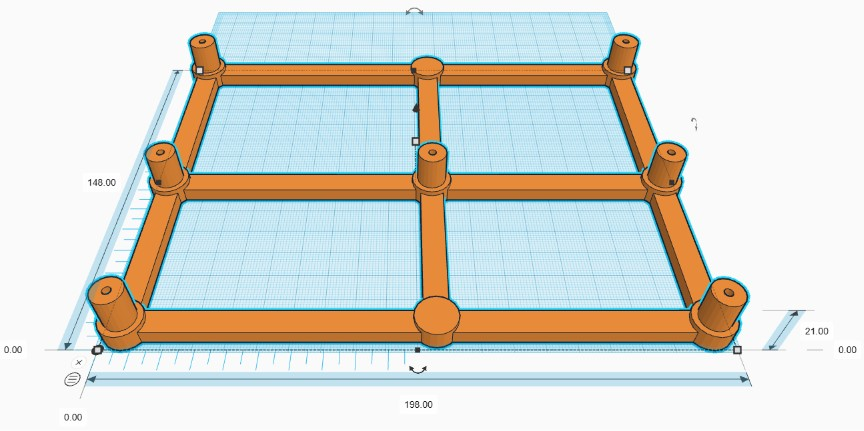
\includegraphics[scale=0.4]{./imagenes/3d_base.jpg}
    \caption{Base plástica 3D para el montaje de la placa de la fuente.}
    \label{F:base3d_fuente}
\end{figure}

\subsection{Sección de interfaz con el usuario}
El componente en cuestión es un pequeño contenedor de color amarillo y negro, ubicado en uno de los laterales del gabinete principal fig \ref{F:caja_usuario}. Este contenedor alberga las bornes de conexión, donde se disponen los terminales que permitirán la vinculación de la carga externa al sistema. \par
Para garantizar una comunicación fluida entre este módulo y el resto de los componentes de la fuente, se ha optado por utilizar un cable de 40 pines. Este tipo de cable, originalmente diseñado para discos duros con interfaz paralela (PATA), resulta ideal para este proyecto debido al elevado número de conexiones necesarias y la robustez que añade a los conductores acoplando todos estos en una sola ficha. En concreto, 16 de estos pines están dedicados a gestionar la comunicación entre el teclado, el encoder y la pantalla, elementos clave en la configuración y monitoreo de la fuente de tensión mientras que el resto de pines no tendrán propósito general y serán asignados a \textit{GND} y a \textit{$V_{CC}$} para fines varios. \par

\begin{figure}[H]
    \centering
    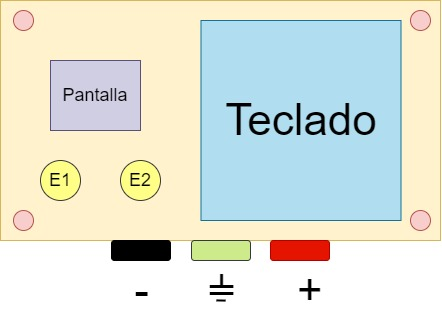
\includegraphics[scale=0.4]{./imagenes/caja_usuario.jpg}
    \caption{Vista superior del panel de control del usuario.}
    \label{F:caja_usuario}
\end{figure}
En base a la necesidad de albergar el teclado, la pantalla y los encoders, se diseñó una tapa en 3D con la disposición indicada en la figura \ref{F:caja_usuario}. \par 
\begin{figure}[H]
    \centering
    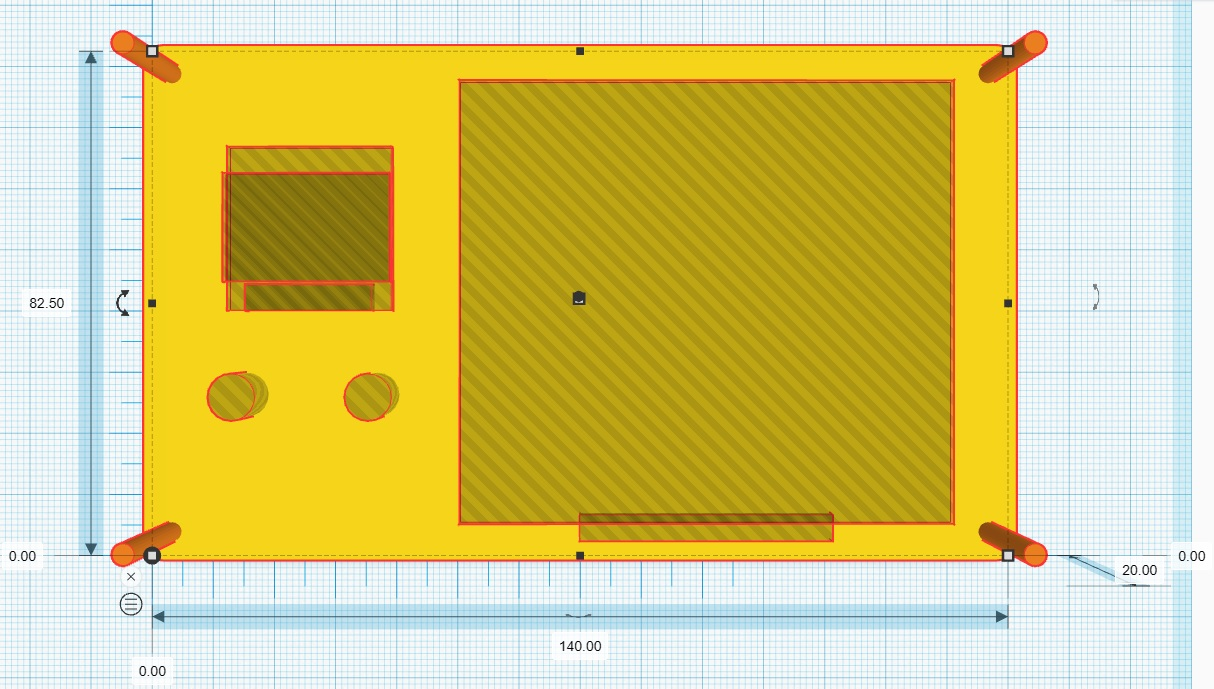
\includegraphics[width=0.6\textwidth]{./imagenes/Tapa_interfaz.jpg}
    \caption{Diseño en 3D de la tapa de la interfaz donde irán montados los módulos.}
    \label{F:Tapa_interfaz}
\end{figure}

\subsection{Correcciones Adicionales}
En esta sección se detallan algunos de los ajustes y correcciones menores que fueron implementados y desarrollados adecuadamente en otras partes del documento. Estos cambios fueron cruciales para optimizar el rendimiento, mejorar la fiabilidad y asegurar la claridad tanto en el diseño físico como en la programación. A continuación, se enumeran los principales aspectos abordados:
\begin{itemize}
    \item \textbf{Ajuste de constantes del controlador:} Se realizaron ajustes finos en las constantes del controlador, lo cual permitió mejorar la precisión y estabilidad del sistema de control. Estos ajustes fueron necesarios para optimizar la respuesta del sistema ante diferentes condiciones de carga y mejorar la robustez del control.
    \item \textbf{Reestructuración del código de programación:} El código de programación del \textit{Arduino Nano} fue reestructurado con el objetivo de optimizar su desempeño, simplificar su lógica y mejorar su comprensión. Esta reestructuración incluyó la eliminación de redundancias, la modularización de funciones clave y la implementación de buenas prácticas de codificación, lo que resultó en un código más eficiente y fácil de mantener.
    \item \textbf{Corrección de huellas PCB de componentes:} Se realizaron correcciones en las huellas PCB de varios componentes para asegurar un ajuste preciso y una correcta conexión en el diseño final. 
    \item \textbf{Redistribución de pistas, pines y componentes:} Se llevó a cabo una redistribución estratégica de las pistas, pines y componentes en el PCB, con el fin de mejorar el flujo de señales, reducir el ruido eléctrico y optimizar el espacio disponible en la placa. Esta redistribución también contribuyó a mejorar la disipación térmica y la accesibilidad para futuras modificaciones o reparaciones.
\end{itemize}

\section{Versión final del PCB}
En base a las correcciones mencionadas en la sección anterior, se presenta en la figura \ref{F:PCB_prototipo2} los PCBs diseñados. En el principal se ha agregado en la parte inferior derecha la sección correspondiente a la conexión con la interfaz de usuario. Fue necesario reubicar el Arduino Nano de forma horizontal para poder enrutar todas las pistas y utilizar la menor cantidad de puentes posibles. \par 
La sección de la derecha corresponde al PCB que se encontrará en la interfaz de usuario. El propósito del mismo será poder distribuir todas las conexiones a los módulos adecuados.
\begin{figure}[H]
    \centering
    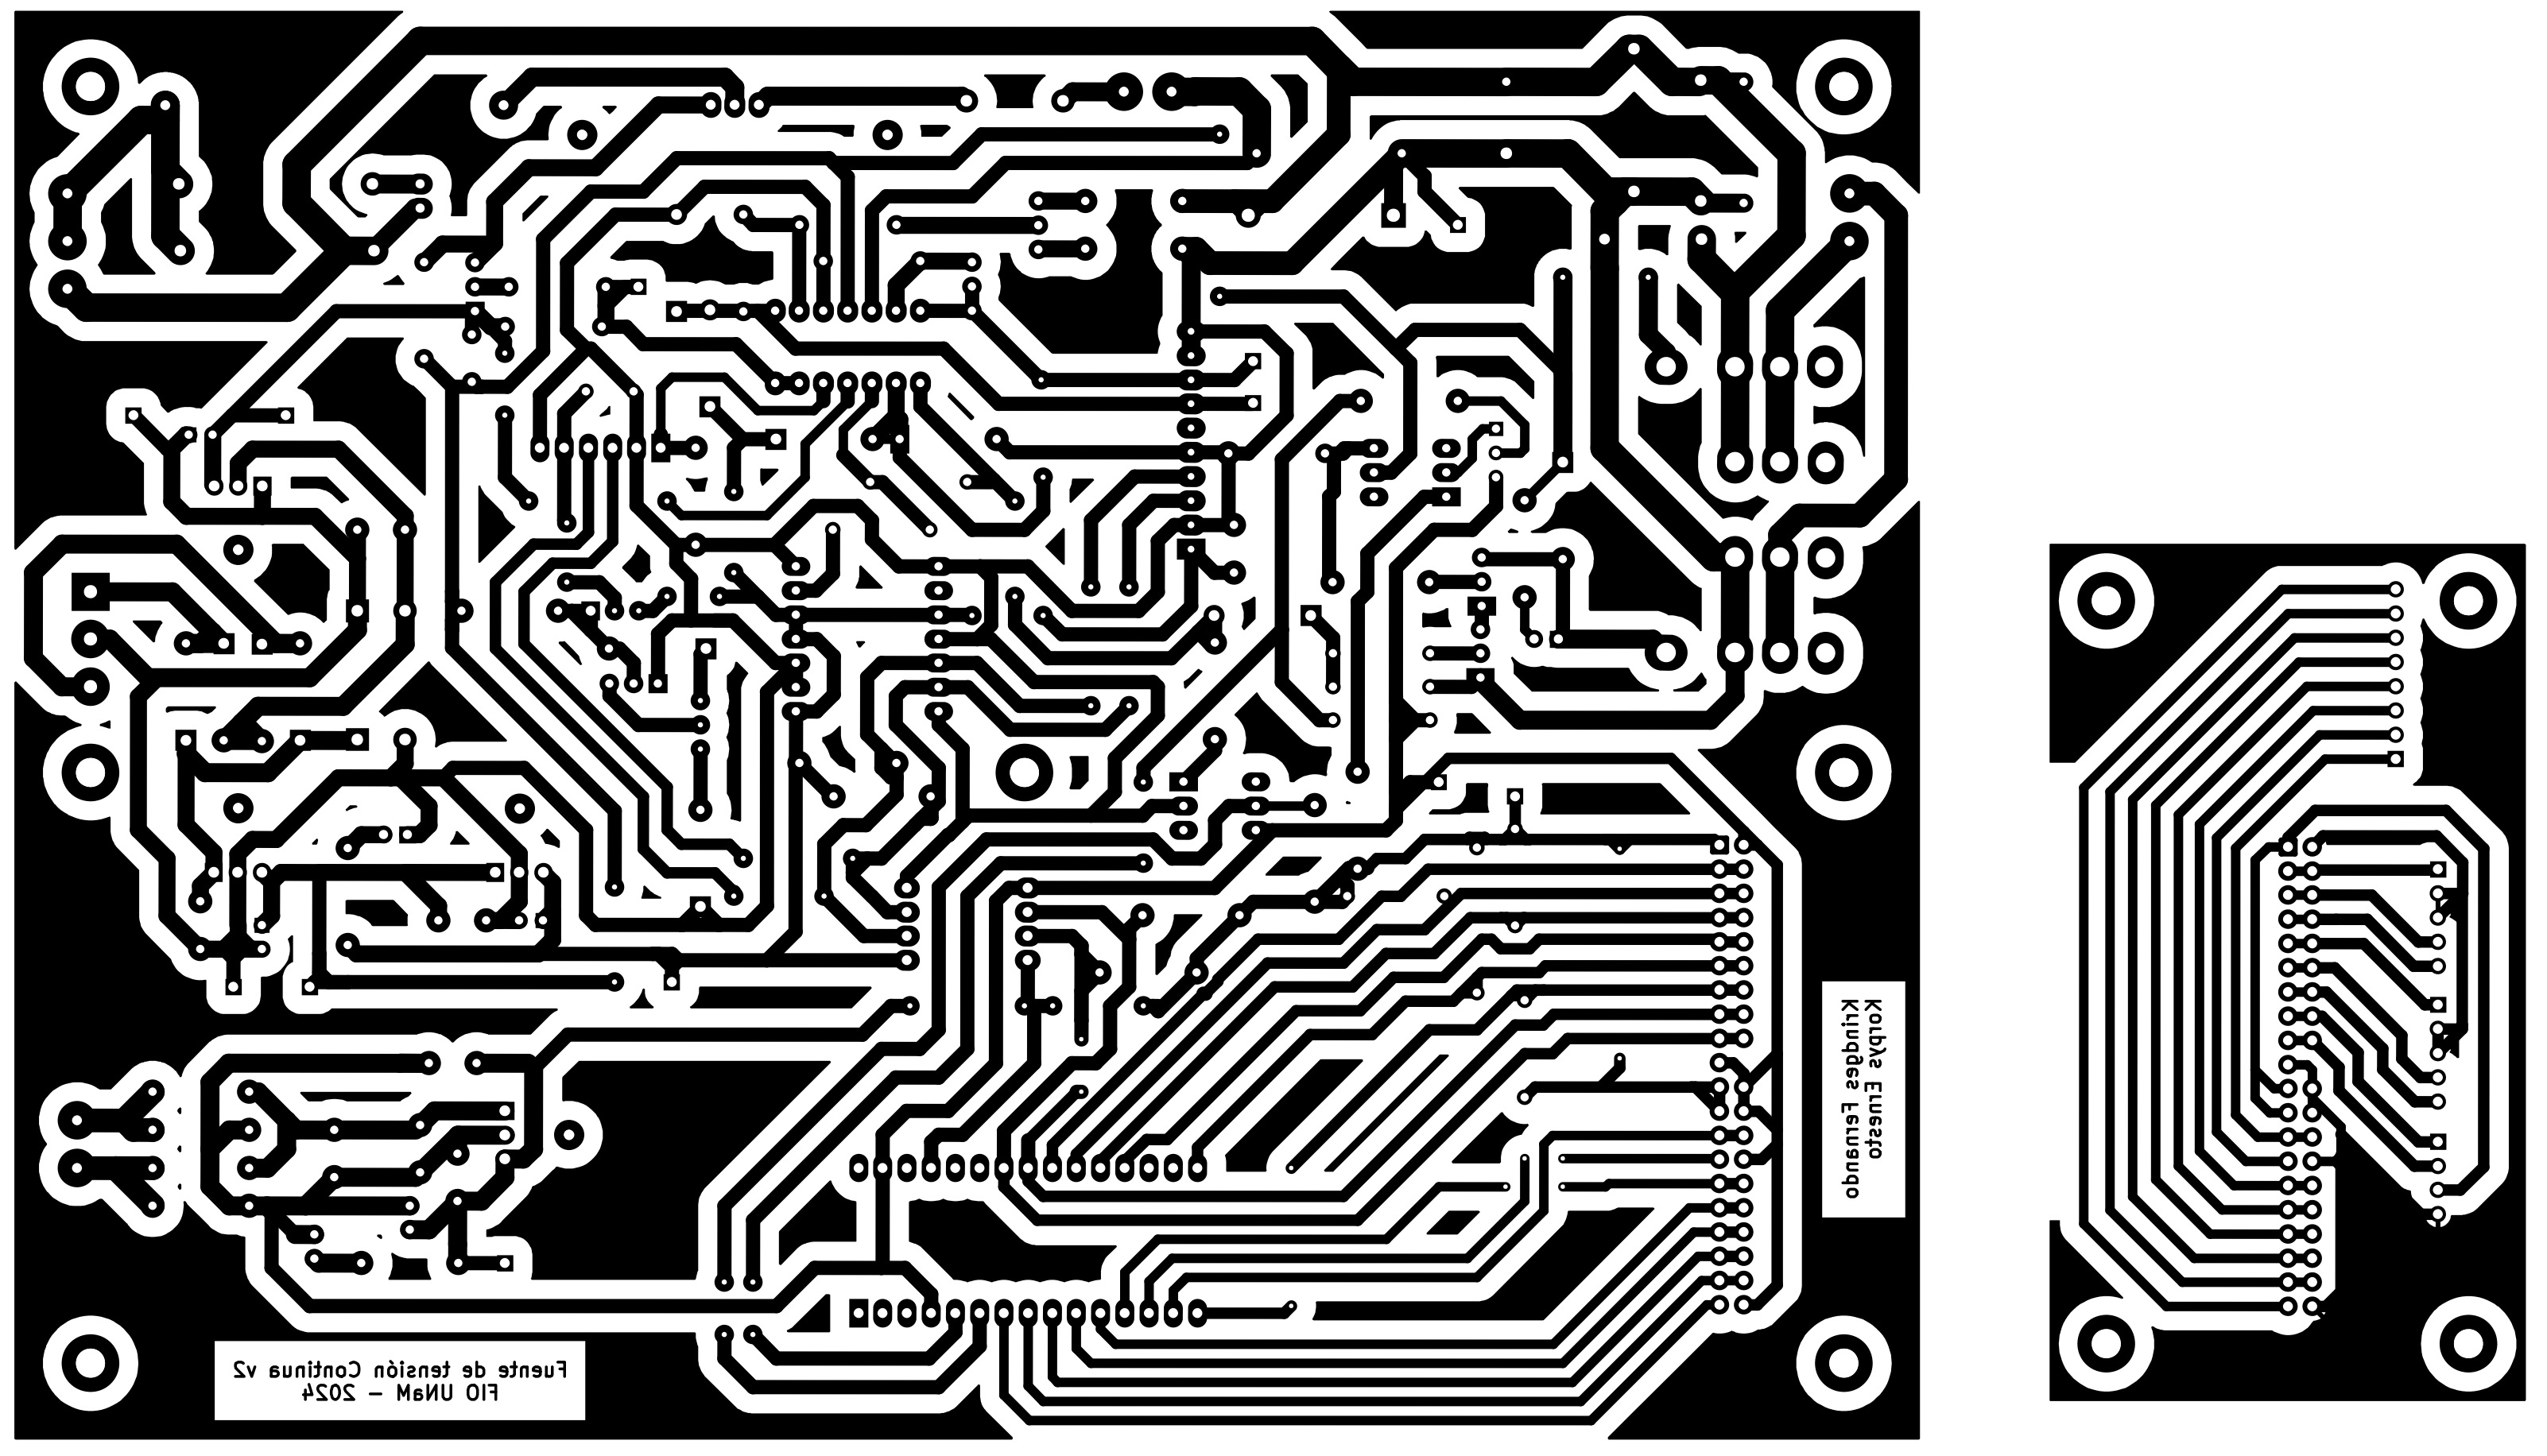
\includegraphics[width=\textwidth]{./imagenes/PCB_prototipo2.jpg}
    \caption{PCB de la fuente de tensión diseñada y de la interfaz de usuario}
    \label{F:PCB_prototipo2}
\end{figure}\par 
Mientras que en la figura \ref{F:3D_v2} se puede observar una vista en 3D de los PCB mencionados.
\begin{figure}[H]
    \centering
    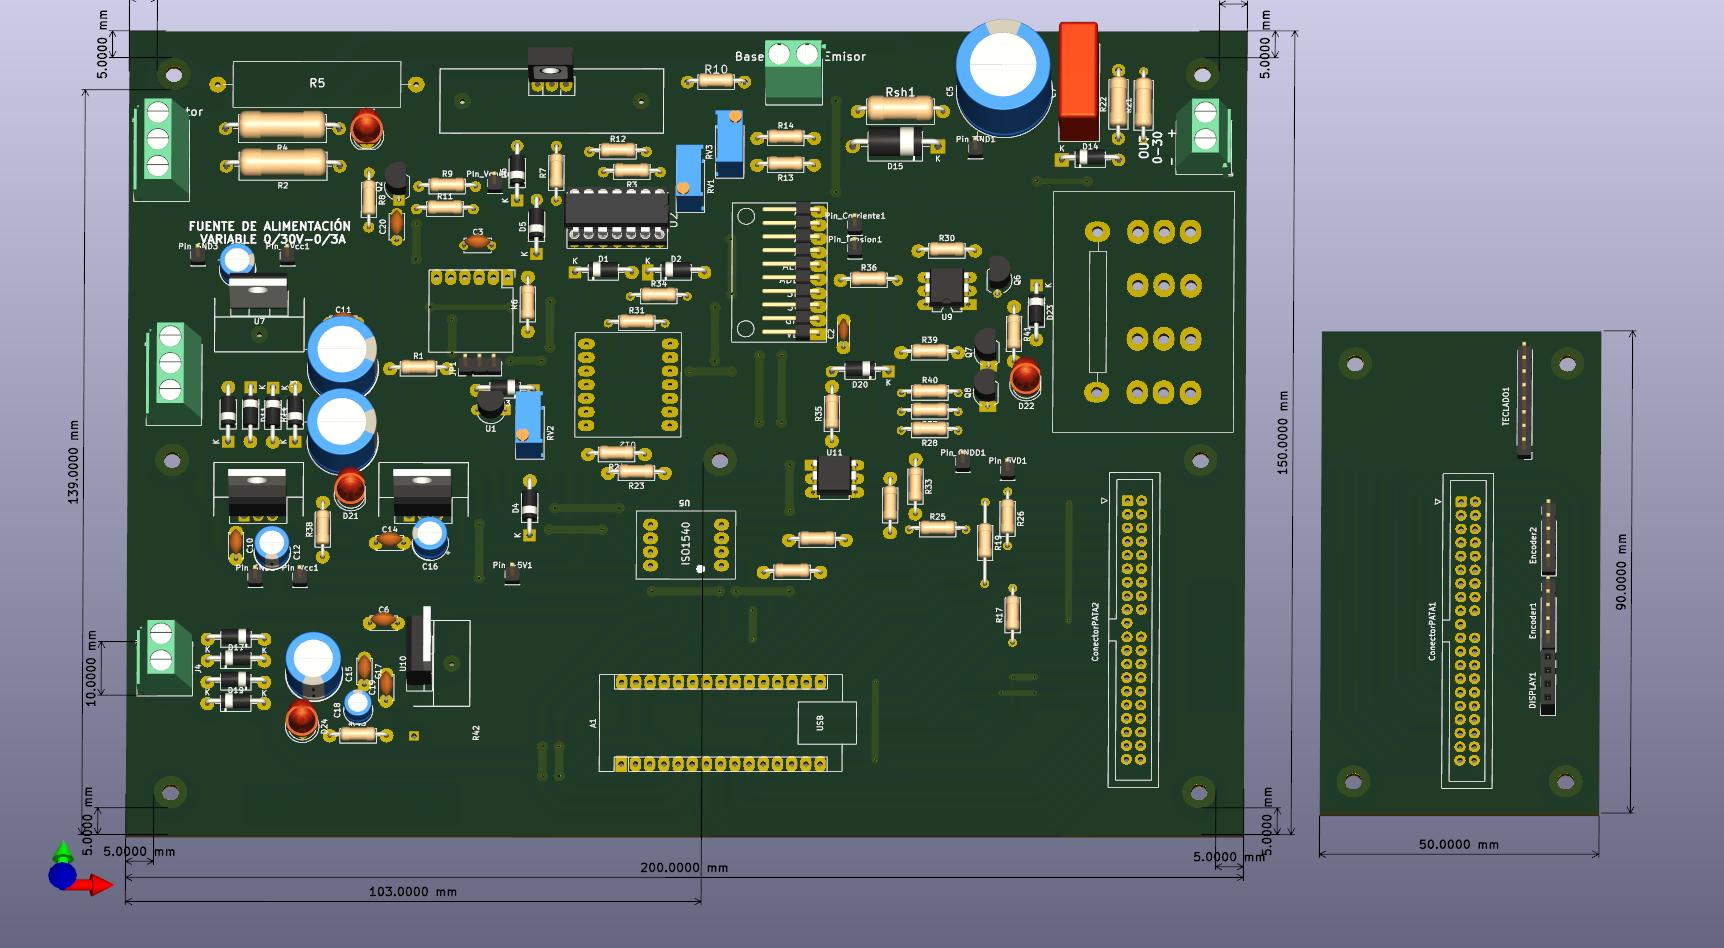
\includegraphics[width=\textwidth]{./imagenes/3D_v2.jpg}
    \caption{Vista en 3D de la versión final del PCB}
    \label{F:3D_v2}
\end{figure}


\chapter{Instrucciones de uso.}
% ----------------------

\label{C:Forma de operar la fuente DC}

\section{Procedimiento de utilización de la fuente}

Esta sección del informe detalla el procedimiento adecuado para la operación del equipo bajo condiciones normales. Se describen los pasos necesarios desde la energización de los transformadores hasta la configuración de los valores, con el fin de garantizar un funcionamiento seguro del equipo.\par 

\begin{enumerate}
    \item Energización de los transformadores.
    \item Inicialización del menu en el display.
    \item Tecla B para moverse sobre el menú.
    \item Tecla A para configurar la protección de desconexión de carga por valor de corriente máximo.
    \item Selector de modo. (Tensión; Corriente; Rampa)
    \item Tecla C para confirmar el modo escogido.
    \item Tecla A para entrar al modo de edición de valores.
    \item Cargar Valores con teclas numéricas.
    \item Tecla \# para poner en marcha la fuente desde la pantalla del modo actualizando las referencias y habilitando la conexión de la carga.
    \item Tecla * para activar el ajuste mediante el uso de \textit{encoder}.
    \item Desactivar el modo de funcionamiento con tecla D en el menu inicial.
\end{enumerate}

\subsection{Diagrama de control de funcionamiento.}

El diagrama de control del funcionamiento es una representación visual esencial que ilustra de manera clara y concisa los pasos y procesos involucrados en el manejo adecuado de un sistema o equipo. Este tipo de diagrama proporciona una guía visual detallada que facilita la comprensión y la ejecución de las tareas necesarias para operar el equipo de manera eficiente. El que se encuentra a continuación en la Figura \ref{F:funcionamiento_normal} resume lo desarrollado en la parte superior de cual sería el procedimiento normal de utilización sin entrar en detalle acerca de errores y fallas imprevistas. 

\begin{figure}[H]
    \centering
    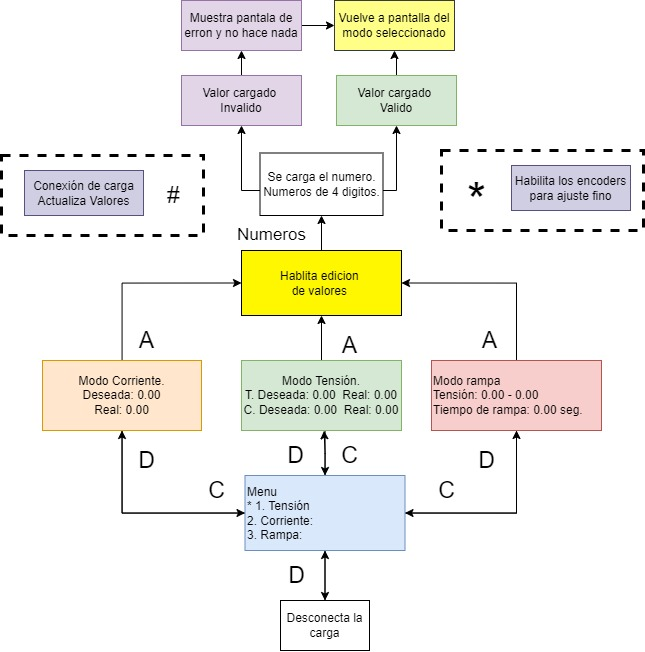
\includegraphics[scale=0.6]{./imagenes/MoverseSobreMenu.jpg}
    \caption{Diagrama de bloques del funcionamiento estándar.}
    \label{F:funcionamiento_normal}
\end{figure}

\section{Uso de teclado} 
El teclado es una interfaz fundamental en el proceso de interacción del usuario con la fuente de alimentación, permitiendo la configuración de parámetros y el control de diferentes modos de operación. Cada tecla tiene asignada una función específica para facilitar la navegación y la manipulación de la configuración. A continuación, se presenta un resumen de la función que realiza cada tecla:
\begin{itemize}
    \item A: Editar valores.
    \item B: Moverse sobre el menú.
    \item C: Confirmar.
    \item D: Volver atrás.
    \item *: Alternar entre teclado y \textit{encoder} para la configuración de la referencia.
    \item \#: Poner en marcha el modo.
    \item Número: Valores numéricos.
\end{itemize}
Estas funciones se ven representadas en la Figura \ref{F:funcionamiento_normal} donde se muestra como con la pulsación de una tecla se genera la transición entre una pantalla a otra.

\section{Pantallas Disponibles} 
En el display se encuentran disponibles seis pantallas distintas, cada una con un propósito específico para la interacción del usuario con la fuente. A continuación, se detalla el contenido y la función de cada una. \par 
Esta estructura proporciona al usuario una interfaz intuitiva y clara para interactuar con la fuente, facilitando la configuración y el monitoreo de los parámetros de salida.\par 
\begin{enumerate}
    \item \textbf{Pantalla Principal - Menú Principal}: Esta pantalla representa el menú principal desde el cual se puede navegar para configurar la fuente. Mediante un puntero, el usuario puede seleccionar el modo de operación deseado.
    \item \textbf{Pantalla de Modo Tensión}: Al seleccionar este modo, la pantalla mostrará los valores configurados de tensión y corriente. Además, proporcionará una visualización en tiempo real de las magnitudes de registradas a tiempo real que se actualiza cada un segundo.
    \item \textbf{Pantalla de Modo Corriente}: Similar al modo de tensión, esta pantalla muestra los valores configurados para la corriente. No incluye un campo para la tensión deseada, ya que se activa exclusivamente el modo de corriente.
    \item \textbf{Pantalla de Modo Rampa}: Aquí se visualizan los valores de tiempo y tensión configurados, junto con los valores registrados en tiempo real y el tiempo transcurrido desde el inicio del modo de rampa.
    \item \textbf{Pantalla de Carga Inválida}: Esta pantalla muestra un mensaje de error cuando los parámetros cargados no son válidos dentro de los límites constructivos de la fuente.
    \item \textbf{Pantalla de Carga de Valores}: En esta pantalla se muestran los valores deseados de los parámetros. Se pueden cargar uno a la vez utilizando el teclado alfanumérico.
    \item \textbf{Pantalla de Error}: Ocurrido algún fenómeno que dispare el valor de corriente a uno superior al configurado en la protección, indicará al usuario de este acontecimiento además de bloquear el funcionamiento normal.
\end{enumerate}

\section{Rangos límite y zonas de operación}
A su vez se han establecido los valores límites mínimos y máximos para garantizar la operación adecuada de la fuente de alimentación y la implementación efectiva del algoritmo de control. Estos valores son los siguientes:

\begin{table}[h!]
\centering
\begin{tabular}{|c|c|c|c|c|c|}
\hline
    \textbf{Modo}   & \multicolumn{2}{c|}{\textbf{Tensión}} & \multicolumn{1}{c|}{\textbf{Corriente}} & \multicolumn{2}{c|}{\textbf{Rampa}} \\ \hline
       & \textbf{Tensión}  & \textbf{Corriente} & \textbf{Corriente} & \textbf{Tensión} & \textbf{Tiempo} \\ \hline
\textbf{Máximo} &30V            &3A             &3A                &30V             &2s               \\ \hline
\textbf{Mínimo} &3V             &200mA          &200mA             &3V              &2s               \\ \hline
\end{tabular}
\caption{Rangos máximos y mínimos de operación para los diferentes modos.}
\end{table}












\chapter{Resultados experimentales.}
% ----------------------

\label{C:Resultados_experimentales.}

\section{Resultados para el modo de tensión}
En esta sección se evalúa el desempeño de la fuente en su primer modo de operación, donde se configura el nivel de tensión de salida deseado y se establece una corriente máxima de salida. Si la corriente supera el valor límite, la fuente ajustará automáticamente la tensión de salida para evitar exceder el flujo de corriente permitido. \par  
Se realizaron varias pruebas para analizar el comportamiento de la fuente bajo distintas condiciones operativas. Los resultados obtenidos permiten delimitar las características de funcionamiento del sistema en escenarios típicos de operación. \par 
\subsection{Valor de carga fijo al energizar}
En esta subsección se presentan los resultados obtenidos al energizar la fuente con una carga fija previamente conectada. El objetivo de esta prueba es observar el comportamiento inicial de la tensión de salida al aplicar la carga y verificar que el sistema mantiene el nivel de tensión configurado sin exceder los límites de corriente establecidos.\par
En las Figuras \ref{F:Energizacion15} y \ref{F:Energizacion25} se muestran los resultados obtenidos \textbf{utilizando una carga resistiva de aproximadamente $30\Omega$}. La prueba se realizó configurando la fuente en 15V y 25V respectivamente. En donde en los laterales de las figuras se puede identificar la magnitud representada, \textbf{siendo la \textit{tensión a la salida} de la fuente en \textbf{azul} y la \textit{acción de control} en \textbf{rojo}}. 
\begin{figure}[htbp]
    \centering
    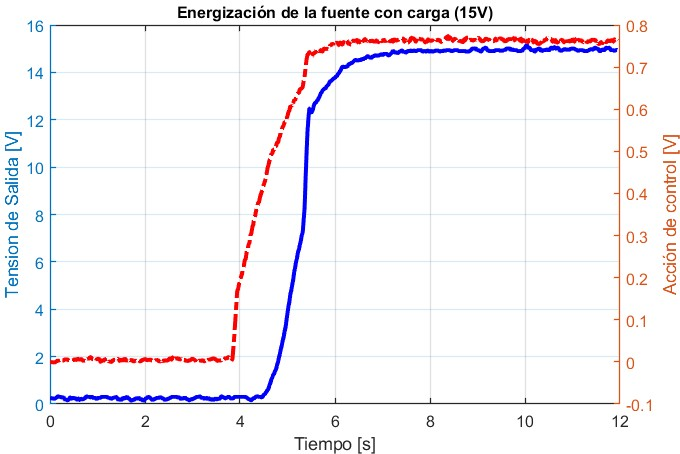
\includegraphics[width=0.8\textwidth]{./imagenes/Energizacion15.jpg}
    \caption{Respuesta obtenida al energizar la fuente configurada en 15V con una carga de conectada.}
    \label{F:Energizacion15}
\end{figure}

\begin{figure}[htbp]
    \centering
    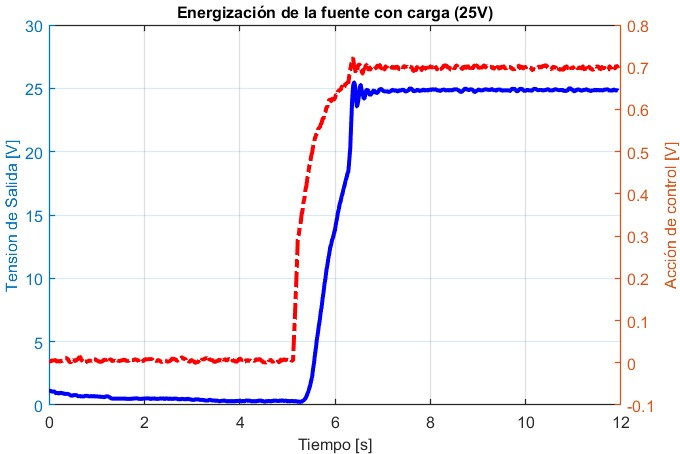
\includegraphics[width=0.8\textwidth]{./imagenes/Energizacion25.jpg}
    \caption{Respuesta obtenida al energizar la fuente configurada en 25V con una carga conectada.}
    \label{F:Energizacion25}
\end{figure}\par 
Los gráficos muestran una respuesta transitoria satisfactoria, alcanzando el valor de referencia con un tiempo de asentamiento cercano a un segundo. Además, no se observa sobrepaso, lo cual indica que la fuente opera de manera estable bajo las condiciones evaluadas.\par 

\subsection{Conexión de carga}
En esta subsección se presentan los resultados obtenidos al conectar una carga con la fuente ya energizada.  El objetivo de esta prueba es evaluar la capacidad del sistema para ajustar rápidamente la tensión de salida al pasar de una condición sin carga (vacío) a una con carga. \par
A continuación, se muestran las Figuras \ref{F:Conexion15} y \ref{F:Conexion25}, donde se observan las respuestas del sistema para dos valores de tensión de salida diferentes: 15V y 25V.\par 

\begin{figure}[htbp]
    \centering
    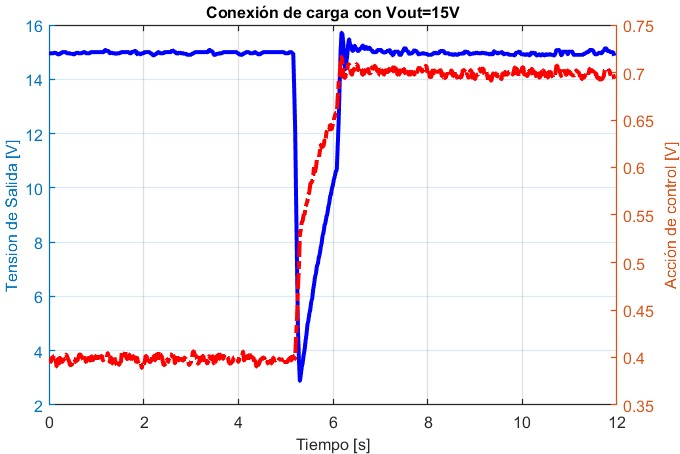
\includegraphics[width=0.8\textwidth]{./imagenes/Conexion2.jpg}
    \caption{Respuesta obtenida al pasar del estado de vacío al de carga con Vout=15V.}
    \label{F:Conexion15}
\end{figure}\par 

\begin{figure}[htbp]
    \centering
    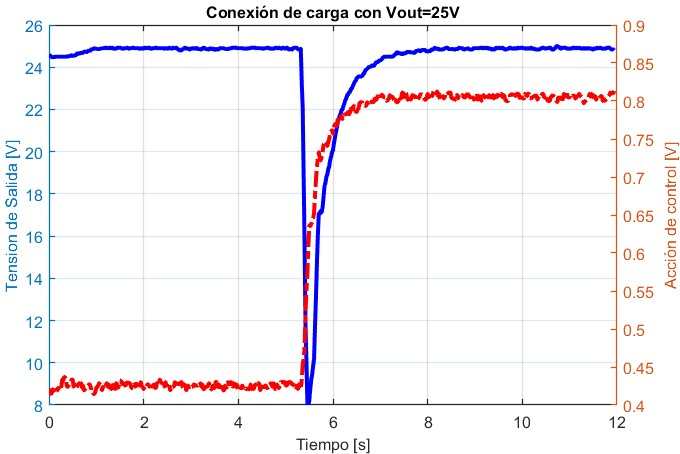
\includegraphics[width=0.8\textwidth]{./imagenes/Conexion1.jpg}
    \caption{Respuesta obtenida al pasar del estado de vacío al de carga con Vout=25V.}
    \label{F:Conexion25}
\end{figure}\par 

Los gráficos muestran una rápida respuesta del algoritmo de control, ajustando la acción de control para mantener la tensión de salida en el valor deseado. En el caso de la prueba con 15V, se observa un ligero sobrepaso, mientras que en la prueba con 25V no hay sobrepaso apreciable. Esta diferencia podría deberse al uso de ganancias más pequeñas en el rango de voltajes más altos. Aun así, en ambos casos, la respuesta es satisfactoria y dentro de los márgenes aceptables para un funcionamiento estable. \par


\subsection{Desconexión de carga}
En esta subsección se analiza el comportamiento de la fuente al desconectar una carga mientras está en funcionamiento. La prueba tiene como objetivo observar cómo responde la fuente ante una desconexión repentina y si es capaz de estabilizar la tensión de salida sin generar sobrecargas o picos no deseados.\par
Las Figuras \ref{F:Desconexion15} y \ref{F:Desconexion25} muestran los resultados obtenidos al pasar de un estado estacionario con carga conectada a una condición de vacío, es decir, sin carga. A continuación, se analiza el desempeño del sistema en cada caso.\par 
\begin{figure}[htbp]
    \centering
    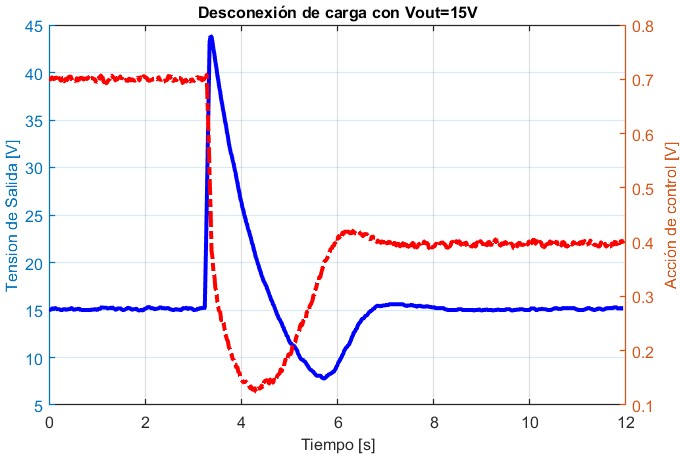
\includegraphics[width=0.8\textwidth]{./imagenes/Desconexion1.jpg}
    \caption{Respuesta obtenida al pasar del estado de carga al de vacío con Vout=15V.}
    \label{F:Desconexion15}
\end{figure}\par 
\begin{figure}[htbp]
    \centering
    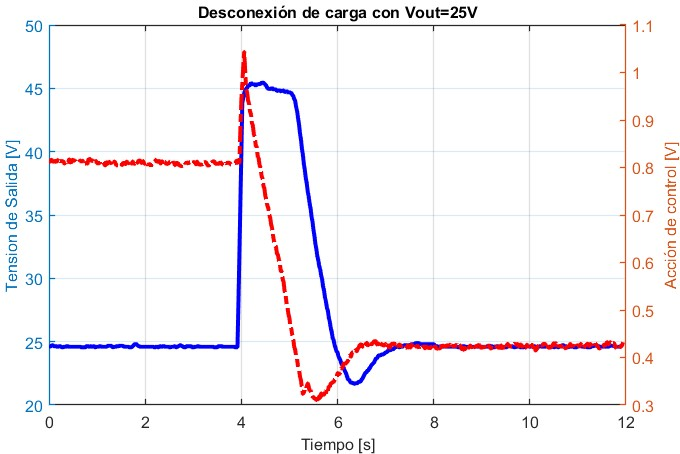
\includegraphics[width=0.8\textwidth]{./imagenes/Desconexion2.jpg}
    \caption{Respuesta obtenida al pasar del estado de carga al de vacío con Vout=25V.}
    \label{F:Desconexion25}
\end{figure}\par 
De los gráficos, se observa que la tensión de salida se incrementa bruscamente tras la desconexión de la carga, alcanzando valores cercanos a los 45V. Esto ocurre a pesar de que la acción de control disminuye rápidamente, lo que indica que, en condición de vacío, sin una carga que consuma la corriente, esta se acumula en el capacitor de salida, provocando el abrupto aumento en la tensión. \par
En el caso de la prueba con 25V, se aprecia una sobretensión de mayor duración en comparación con la prueba de 15V. Ante estas condiciones, se considera necesario añadir una lógica de desacoplamiento de la carga para prevenir que, durante un transitorio, la reconexión de una carga se someta a un valor de tensión superior al esperado. Esta medida es fundamental para evitar posibles daños en los equipos conectados. \par 

\subsection{Prueba con motor de 12 V}
En este apartado se presentan los resultados de las pruebas realizadas al conectar un motor de 12 V a la fuente de alimentación. El objetivo es analizar el comportamiento de la fuente cuando opera con una carga inductiva, así como su capacidad para manejar los picos de corriente generados durante el arranque del motor. \par 
La Figura \ref{F:Motor12} muestra el comportamiento de la tensión de salida cuando se conecta este tipo de carga. Se observa un \textit{ripple} considerable en torno al voltaje de referencia, lo que indica fluctuaciones en la salida mientras el motor está en operación. En esta prueba, el motor se encontraba sin carga mecánica adicional. \par 
\begin{figure}[H]
    \centering
    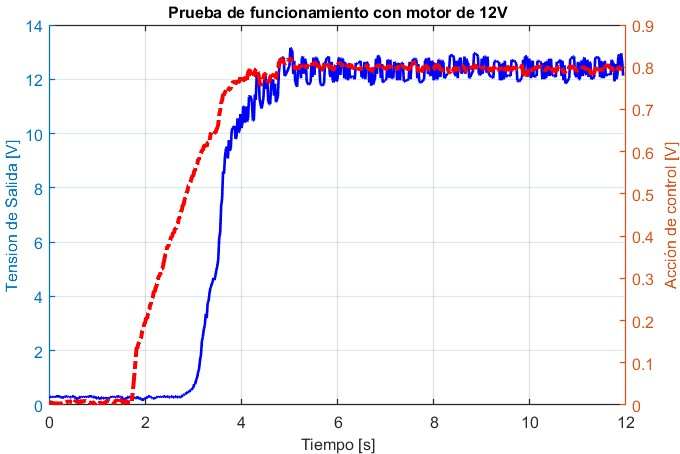
\includegraphics[width=0.8\textwidth]{./imagenes/Motor2.jpg}
    \caption{Prueba de funcionamiento con motor de 12V.}
    \label{F:Motor12}
\end{figure}\par 
El ripple observado sugiere que la fuente podría estar reaccionando a los transitorios causados por la naturaleza inductiva del motor. Es importante mencionar que este tipo de cargas pueden generar corrientes de retorno que podrían afectar la estabilidad de la fuente. \par 

\subsection{Protección por sobrecorriente}
En esta subsección se presentan los resultados de la prueba de protección por sobrecorriente. Para realizar la prueba, se incrementó gradualmente la demanda de corriente hasta superar el límite configurado, lo que activó el mecanismo de protección de la fuente. Este mecanismo reduce la tensión de salida para evitar que la corriente sobrepase el valor máximo establecido. El objetivo es verificar la efectividad del sistema de protección y la estabilidad de su respuesta en condiciones de sobrecarga. \par 
En la Figura \ref{F:Pcorriente1} se observa cómo la fuente disminuye el voltaje de salida cuando la corriente alcanza el valor límite de 1A. Durante la prueba, se realizó un barrido gradual variando los valores de resistencia de la carga, y la respuesta del sistema fue satisfactoria. Sin embargo, se sugiere realizar un ajuste fino en el acondicionador de señal de corriente para optimizar aún más el control del límite.\par 

\begin{figure}[H]
    \centering
    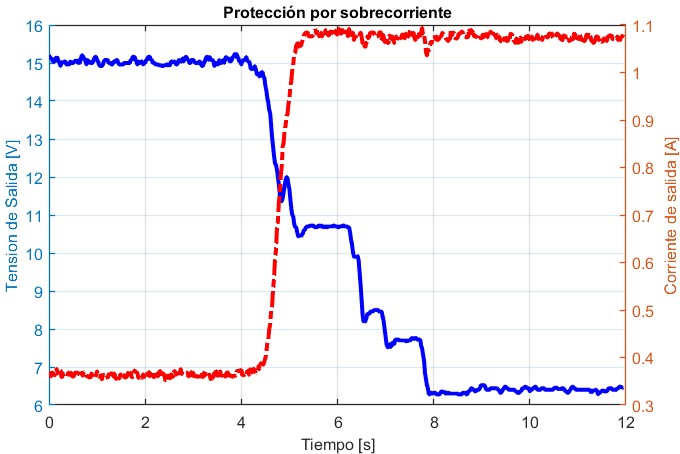
\includegraphics[width=0.8\textwidth]{./imagenes/MedicionConPuntaCorriente_proteccion.jpg}
    \caption{Respuesta obtenida de la protección por sobrecorriente.}
    \label{F:Pcorriente1}
\end{figure}\par 

La Figura \ref{F:Pcorriente2} muestra una situación similar, pero en este caso se conectó abruptamente una carga de $8,2\Omega$ en paralelo a una de $30\Omega$. A pesar de la variación brusca en la demanda de corriente, la respuesta de la fuente fue rápida y adecuada.\par 

\begin{figure}[H]
    \centering
    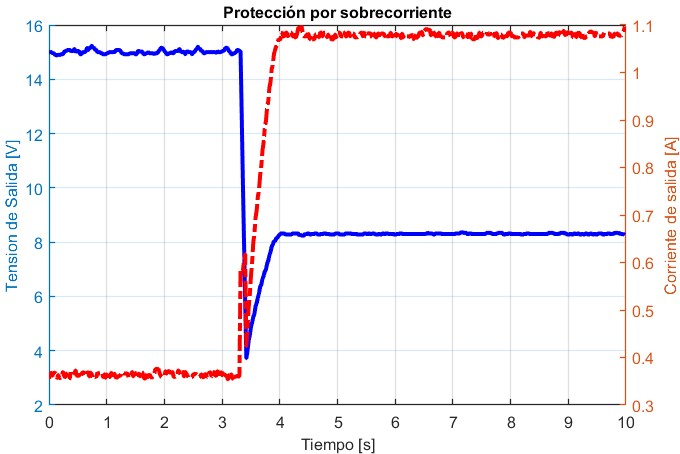
\includegraphics[width=0.8\textwidth]{./imagenes/MedicionConPuntaCorriente_proteccionRapida.jpg}
    \caption{Respuesta obtenida de la protección por sobrecorriente ante la conexión abrupta de una carga.}
    \label{F:Pcorriente2}
\end{figure}\par 

\section{Resultados para el modo de corriente} \label{S:subseccion de corriente}
Este segundo modo de operación implementa un lazo de control que regula la corriente de salida. El usuario especifica el valor de corriente deseado, y la tensión de salida de la fuente se ajusta automáticamente para mantener ese flujo de corriente. Cabe destacar que es importante mantener la carga conectada antes de energizar la salida. Si la carga está desconectada o es demasiado pequeña, el lazo de control no logrará alcanzar su referencia, lo que incrementará su acción integral. Esto resulta en una mayor tensión aplicada a la base de los transistores, pudiendo llevar la tensión de salida a niveles cercanos a $43V$. \par 
Para las pruebas, se utilizó una \textbf{carga resistiva variable}, configurando la corriente en $1A$ para observar el comportamiento transitorio del algoritmo de control. Los resultados obtenidos se muestran en la Figura \ref{F:Lcorriente1}, representandose en \textbf{\textbf{azul} la \textit{tensión} a la salida de la fuente y en \textbf{rojo} la \textit{corriente} a la salida de la misma}.
\begin{figure}[H]
    \centering
    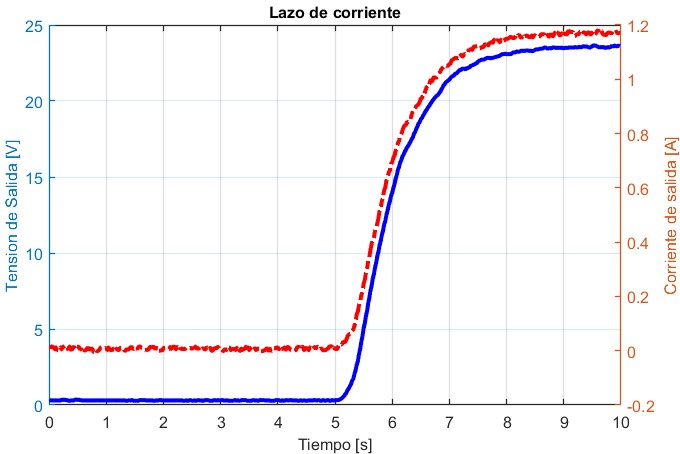
\includegraphics[width=0.8\textwidth]{./imagenes/LazoCorriente.jpg}
    \caption{Respuesta obtenida del modo corriente para una referencia de 1A.}
    \label{F:Lcorriente1}
\end{figure} \par 
Las gráficas muestran una respuesta sobreamortiguada, con un tiempo de asentamiento cercano a los dos segundos. Aunque la respuesta es algo lenta, es adecuada para evitar sobrepasos que podrían dañar los equipos conectados a la salida. Se denota que se requiere un ajuste fino del preset de la etapa acondicionadora de la señal de corriente. \par

\section{Resultados para el modo rampa}
Se realizaron ensayos para verificar el correcto funcionamiento del tercer modo de operación, que corresponde a un perfil de rampa. En este modo, el valor de referencia de tensión se incrementa gradualmente hasta alcanzar el valor fijado por el usuario en un tiempo determinado. \par 
A continuación se presentan las Figuras \ref{F:Rampa24_16} y \ref{F:Rampa24_30}, donde se puede observar la respuesta obtenida en los ensayos. Los experimentos se realizaron utilizando una carga resistiva inferior a $100\Omega$. \par
\begin{figure}[H]
    \centering
    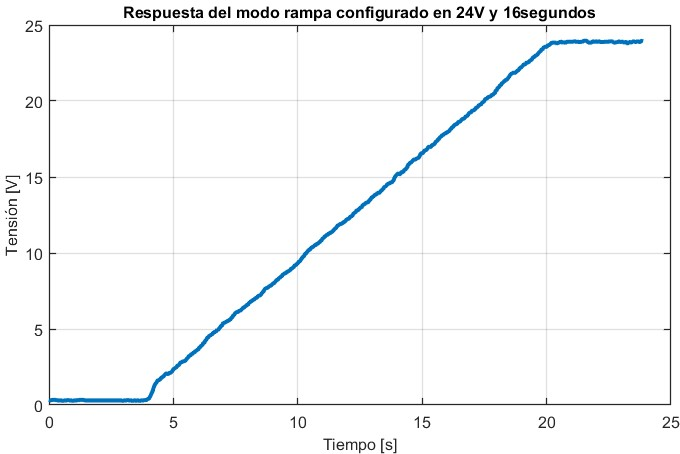
\includegraphics[width=0.8\textwidth]{./imagenes/Rampa_24_16.jpg}
    \caption{Respuesta obtenida del modo rampa para una configuración de 24 V y 16segundos.}
    \label{F:Rampa24_16}
\end{figure}
\begin{figure}[H]
    \centering
    \includegraphics[width=0.8\textwidth]{./imagenes/Rampa_24_30.jpg}
    \caption{Respuesta obtenida del modo rampa para una configuración de 24 V y 30segundos.}
    \label{F:Rampa24_30}
\end{figure}\par 
En las gráficas se puede apreciar un crecimiento lineal de la tensión conforme al tiempo establecido. Se observa un mayor incremento en los primeros instantes de la rampa, lo cual es atribuible a la estrategia de control implementada. Sin embargo, este efecto es insignificante y no compromete el correcto funcionamiento del sistema.\par 

\section{Análisis de la tensión de entrada}
Para determinar el rango de operación de la fuente de alimentación, se analizó el comportamiento de la tensión de entrada rectificada antes del regulador basado en BJT. Este análisis permite evaluar la estabilidad y el margen de operación de los transistores en la zona activa, incluso bajo condiciones de carga variables. \par

Se presentan dos condiciones principales para observar el comportamiento de la tensión de entrada. En primer lugar, se evaluó el funcionamiento en una condición de baja corriente, en torno a 200 mA, como se muestra en la Figura \ref{F:Tension_entrada_12}. En esta figura, se observa que cuando la fuente está desactivada, la tensión rectificada se mantiene cerca de 46 V. Sin embargo, al habilitar la salida y establecer un nivel de tensión dado, la tensión de entrada desciende hasta aproximadamente 34V. Este descenso es aceptable y evidencia un margen de operación adecuado para los transistores, asegurando su funcionamiento en la zona activa incluso si se incrementa la tensión de salida hasta 30 V. \par

\begin{figure}[H]
    \centering
    \includegraphics[width=0.8\textwidth]{./imagenes/Tension_12.jpg}
    \caption{Análisis de la tensión de entrada frente a un punto de operación normal.}
    \label{F:Tension_entrada_12}
\end{figure}\par

La segunda condición analizada corresponde a la corriente de salida máxima, en la que la fuente suministra aproximadamente 3 A. La Figura \ref{F:Vrec_Isal} muestra el análisis de la tensión de entrada bajo esta carga nominal. Al exigir esta corriente, se observa que la tensión de entrada vuelve a caer, similar al caso anterior, pero se mantiene por encima de 34 V. Este resultado confirma que, incluso en condiciones de máxima demanda de corriente, los transistores continúan operando dentro de la zona activa, manteniendo así el margen necesario para una regulación estable. \par

\begin{figure}[H]
    \centering
    \includegraphics[width=0.8\textwidth]{./imagenes/Vrec_Isal.jpg}
    \caption{Análisis de la tensión de entrada frente a una condición de carga nominal.}
    \label{F:Vrec_Isal}
\end{figure}\par 

Finalmente, se analizó el rizado en la tensión de entrada para esta última condición de carga máxima. Para capturar el rizado, se configuró el osciloscopio en modo de acoplamiento de corriente alterna (CA), permitiendo medir exclusivamente el componente de riple. La Figura \ref{F:ripple} muestra los resultados obtenidos, donde se observa un rizado de aproximadamente 2 V pico a pico con una frecuencia cercana a 100 Hz, correspondiente al rectificador de onda completa. Estos valores de rizado son aceptables, confirmando el correcto funcionamiento de la fuente dentro del rango especificado en los objetivos del diseño.

\begin{figure}[H]
    \centering
    \includegraphics[width=0.8\textwidth]{./imagenes/ripple.jpg}
    \caption{Análisis de la tensión de entrada frente a una condición de carga nominal.}
    \label{F:ripple}
\end{figure}\par 



\chapter{Conclusiones y resultados finales.}
% ----------------------

\label{C:Conclusiones y resultados finales.}

\section{Rendimiento de la fuente} 
En primer lugar, la fuente de alimentación diseñada ha demostrado un rendimiento satisfactorio, logrando mantener un nivel de tensión y corriente estable dentro del rango establecido. Los resultados obtenidos muestran que la fuente es capaz de operar en tres modos programables: tensión constante, corriente constante y un modo rampa, lo que permite un mayor control y flexibilidad en su funcionamiento. Estos modos de operación brindan un amplio espectro de aplicaciones, desde pruebas de dispositivos electrónicos hasta la alimentación controlada de cargas críticas.\par
El sistema implementado ha superado con éxito las pruebas de estabilidad y precisión, asegurando un comportamiento confiable bajo diversas condiciones de carga. Además, se destaca que el sistema de control digital permite ajustar los parámetros de salida con gran precisión, lo que es una ventaja significativa frente a sistemas analógicos de características similares.\par
Sin embargo,

\section{Mejoras y limitaciones} 
Recordemos que el proyecto comenzó como una iniciativa de modernización de una fuente de alimentación de naturaleza completamente analógica. Desde esta perspectiva, resulta pertinente realizar algunas comparaciones que permiten visualizar las mejoras obtenidas respecto al modelo anterior como también algunos de los puntos débiles que la limitan en algún sentido.\par

\subsection{Mejoras} 
la implementación de un teclado y encoders, lo que ha simplificado enormemente la programación y el ajuste de parámetros. Esta mejora no solo facilita la interacción con el dispositivo, sino que también contribuye a una mayor precisión en los ajustes de salida. 
Asimismo, se rediseñó la interfaz física de la fuente, logrando una presentación más amigable e intuitiva para el usuario. 
La carcasa de la fuente no solo protege los componentes internos de factores ambientales adversos, sino que también permite una manipulación más segura y eficiente por parte del usuario.\par

\subsection{Limitaciones} 
Sin embargo, a pesar de los avances, se han identificado ciertas limitaciones inherentes al diseño actual. 
Un aspecto que afecta negativamente el rendimiento es el tiempo de estabilización requerido debido a la presencia de un capacitor en la salida. Este componente tiende a provocar un incremento rápido en los valores de tensión, superando la capacidad de respuesta del algoritmo de control, lo que puede ocasionar inestabilidades temporales. 
Otra limitación relevante es la velocidad de muestreo del ADC, que impone restricciones en la capacidad del sistema para responder rápidamente a variaciones de carga o a cambios en los parámetros de salida.

\section{Conclusiones} 
A partir de los resultados obtenidos y del análisis del rendimiento de la fuente, se concluye que un sistema de control totalmente digital, si bien ofrece ciertas ventajas en términos de flexibilidad y precisión, no siempre es la opción más eficiente para la construcción de fuentes de alimentación. Al compararse con fuentes analógicas tradicionales o con fuentes conmutadas (switching), el rendimiento de la fuente digital desarrollada muestra ciertas deficiencias, principalmente en términos de respuesta dinámica y control de estabilidad en situaciones críticas.\par
No obstante, el diseño ha permitido explorar las capacidades de los sistemas de control digital y ha ofrecido una plataforma para futuras mejoras o implementaciones, lo que representa una valiosa experiencia en la integración de tecnologías digitales en el campo del control de potencia.

\section{Retoma del proyecto en un futuro} 
Este informe ha cubierto de manera exhaustiva todas las etapas del desarrollo del proyecto, desde su conceptualización inicial hasta la construcción final del dispositivo. En base a los resultados obtenidos, se puede afirmar que el proyecto ha sido exitoso en términos de cumplir con los objetivos propuestos. Sin embargo, en caso de que se desee retomar este proyecto en el futuro, se presentan a continuación algunos puntos que facilitarán la comprensión y el avance sobre lo ya construido:

\begin{itemize}
    \item El código fuente principal utilizado para el control del sistema, que ha sido cargado en el microcontrolador Arduino Nano, se encuentra disponible en un repositorio de GitHub, lo que asegura la accesibilidad y preservación del software para futuras modificaciones o actualizaciones.
    \item La placa de circuito impreso (PCB) cuenta con múltiples puntos de prueba estratégicamente ubicados. Estos puntos permiten la conexión directa de un osciloscopio, lo que es esencial para realizar ensayos y pruebas de diagnóstico sin necesidad de modificar el diseño original.
    \item En caso de que sea necesario desensamblar la placa o modificar el valor de los potenciómetros, será indispensable recalibrar el sistema de conversión analógico-digital (ADC) para asegurar que los valores medidos coincidan con los valores reales de operación.
\end{itemize}

De esta manera, el proyecto está preparado para ser mejorado o expandido en futuras iteraciones, proporcionando una base sólida sobre la cual desarrollar nuevas funcionalidades o resolver las limitaciones actualmente presentes.

%\chapter{Conclusiones}

\lipsum[5-6]

%\input{contenido/4_clasificacion_y_def.tex}

% 9. BILIOGRAFÍA
\printbibliography[title={Bibliografía}]

% 8. APÉNDICES
\appendix
% si necesitamos agregar algún apéndice activamos esto
%\chapter{Apéndice de ejemplo}
\label{C:anexo-comunicación-serial}

\lipsum[2-4]



\backmatter

%%%%%%%%%%%%%%%%%%%
\end{document}
%%%%%%%%%%%%%%%%%%%
